\newcommand{\MassExclWPr}{3.7\xspace} % in TeV
\newcommand{\MassExclZPr}{3.5\xspace}
\newcommand{\MassExclVPr}{V.V\xspace}
\newcommand{\BulkGMassMin}{1.2\xspace} %UPDATE
\newcommand{\BulkGMassMinXsec}{9\xspace} % in fb
\newcommand{\BulkGMassMax}{5.2\xspace}
\newcommand{\BulkGMassMaxXsec}{0.2\xspace} %UPDATE
\newcommand{\BulkGWWMassMinXsec}{9\xspace} % in fb
\newcommand{\BulkGWWMassMaxXsec}{0.2\xspace}
\newcommand{\BulkGZZMassMinXsec}{13\xspace} % in fb
\newcommand{\BulkGZZMassMaxXsec}{0.2\xspace}
\section{Small bumps and tri-bosons}
In addition to the observation of a $3.4 \sigma$ excess in the search for diboson resonances in the all-hadronic final state by ATLAS~\cite{Aad2015}, not confirmed by subsequent searches, several little bumps near 2 TeV were observed in data collected at center-of-mass energies of 8 and 13 TeV, as illustrated by the dijet invariant mass distributions observed by ATLAS and CMS in Figure~\ref{fig:searchIII:bumps}. These were not statistically significant, and are expected due to statistical fluctuations, however, only a coherent analysis would be able to determine if a new physics signal could be partly responsible for any of these excesses in the dijet invariant mass of V jets.
\begin{figure}[h!] 
    \centering
    %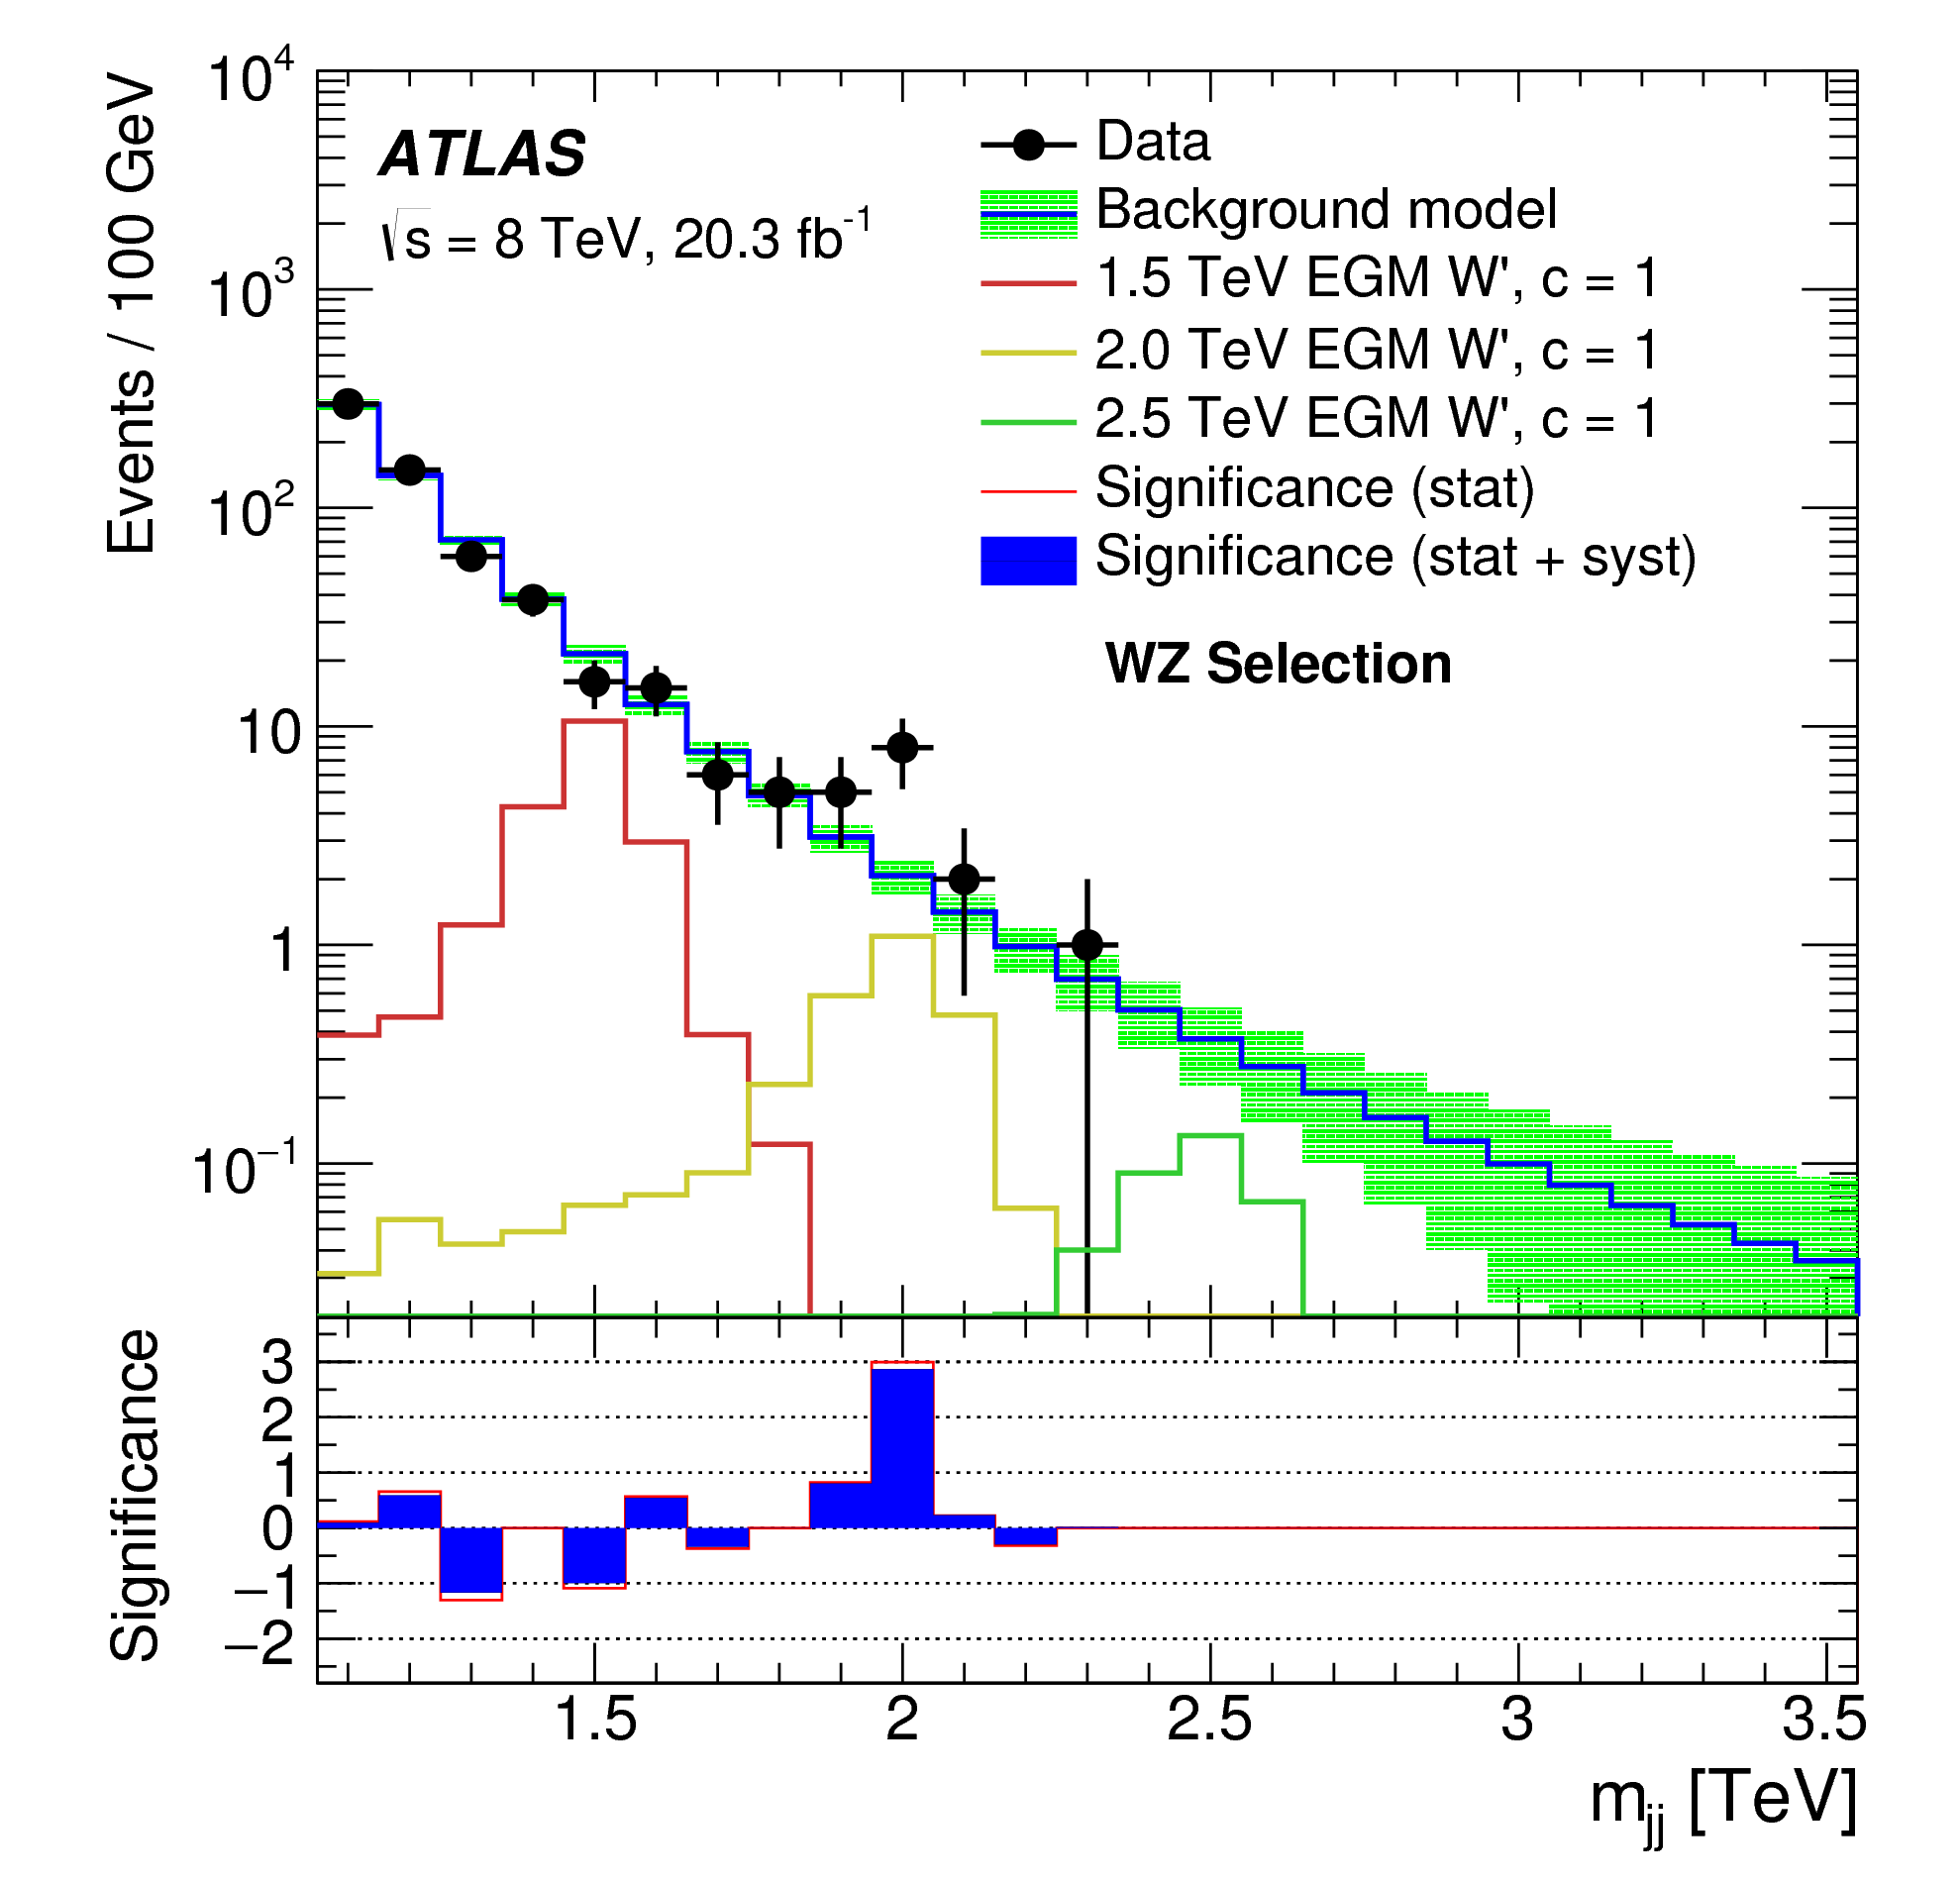
\includegraphics[height=0.3\textwidth]{figures/analysis/search1/misc/atlas_8tev.png}
    %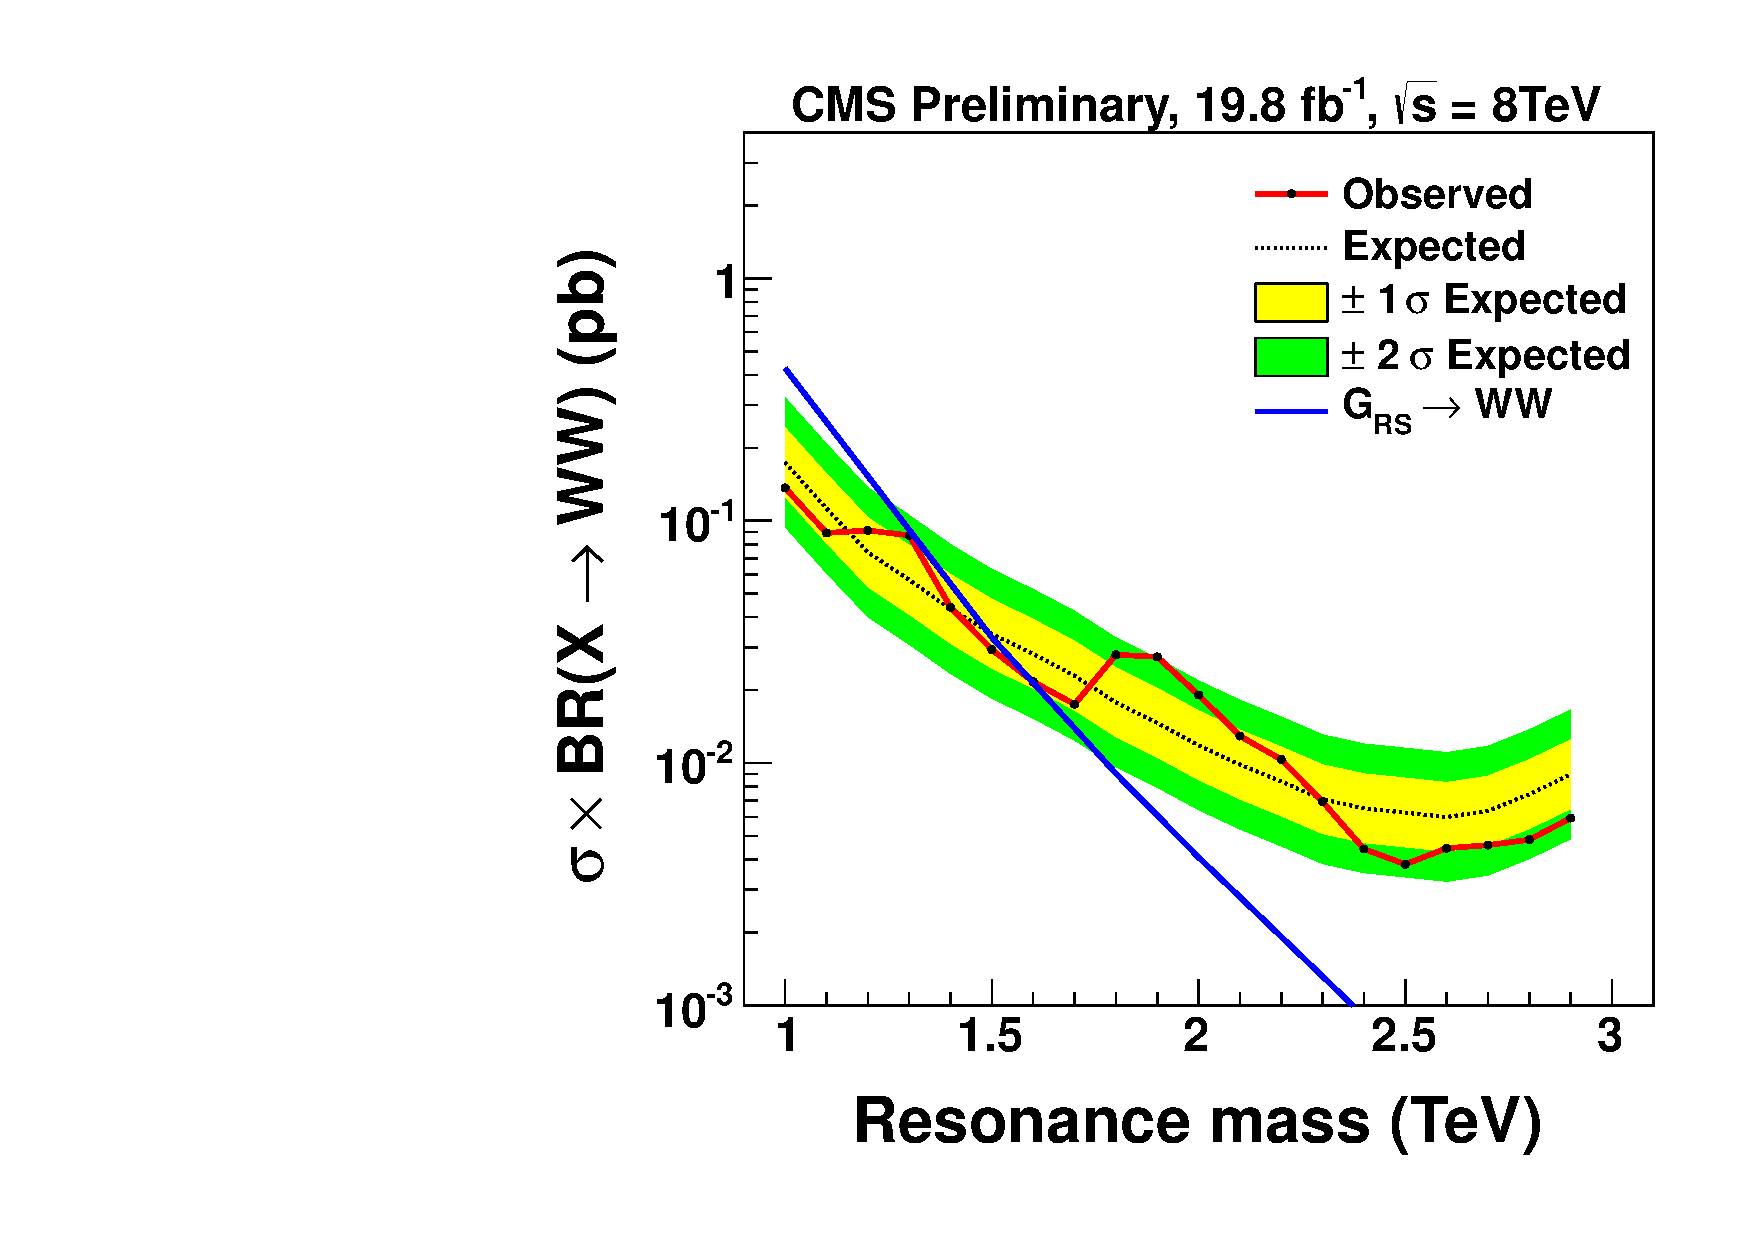
\includegraphics[height=0.3\textwidth]{figures/analysis/search1/misc/EXO-12-024_gWW.pdf}\\
    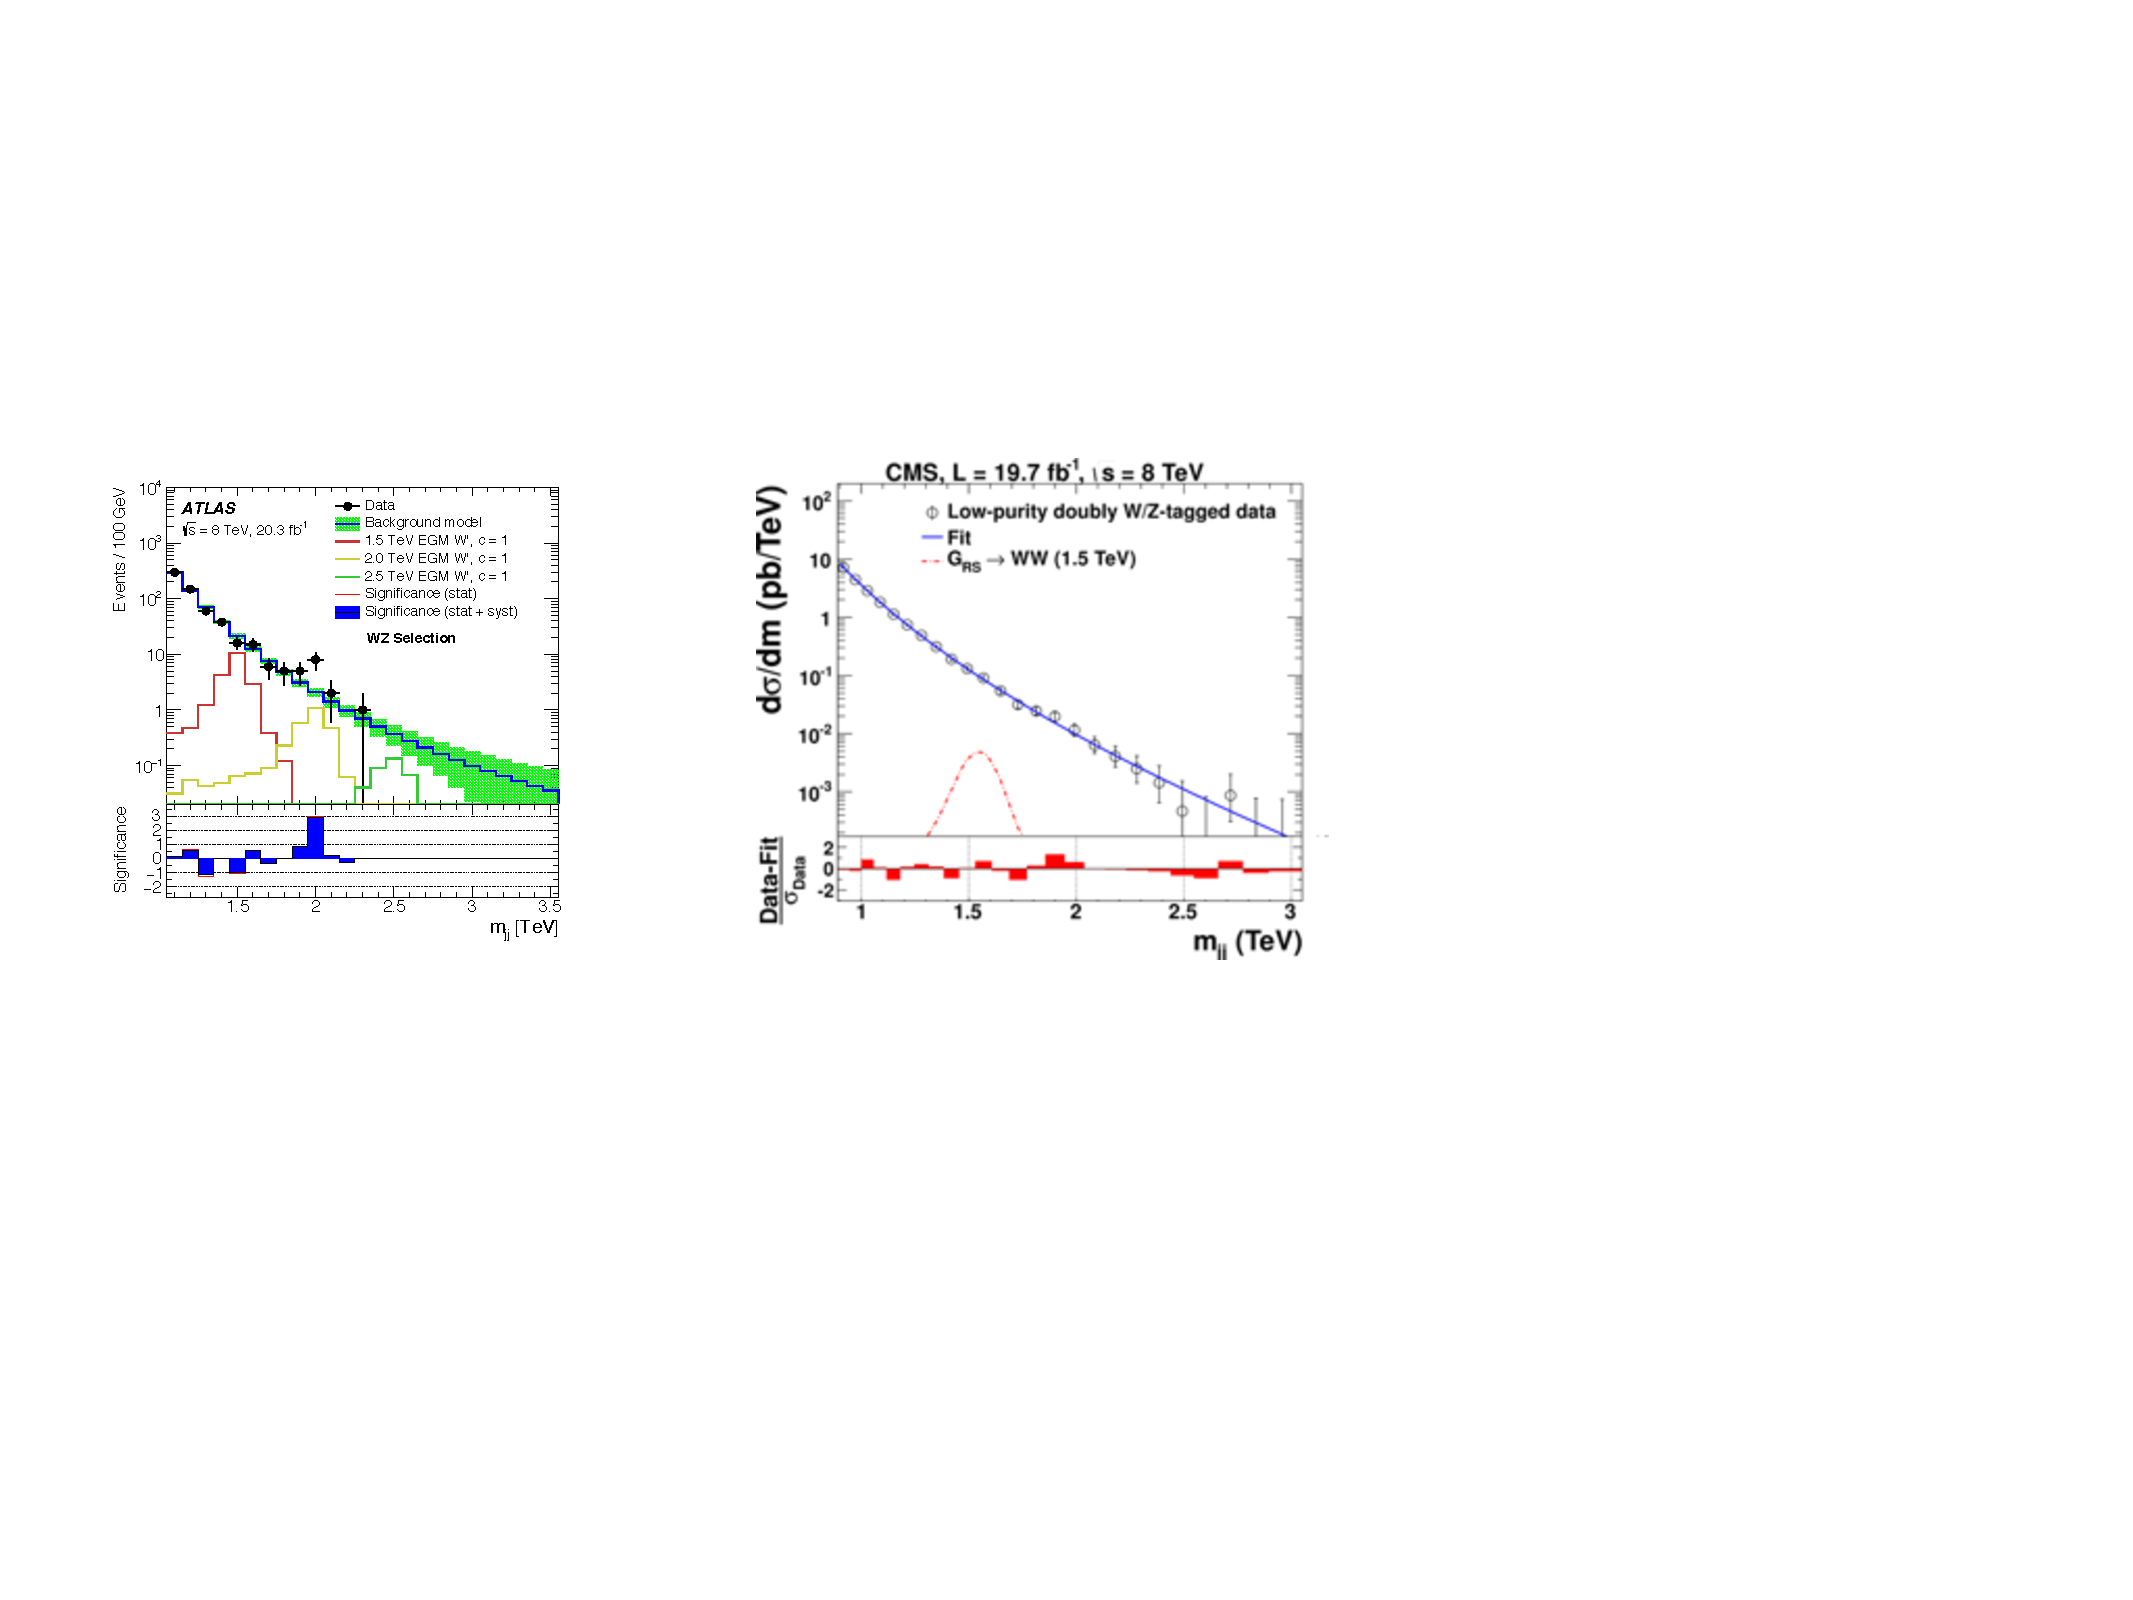
\includegraphics[width=0.69\textwidth]{figures/analysis/search3/misc/bumps2.pdf}\\
    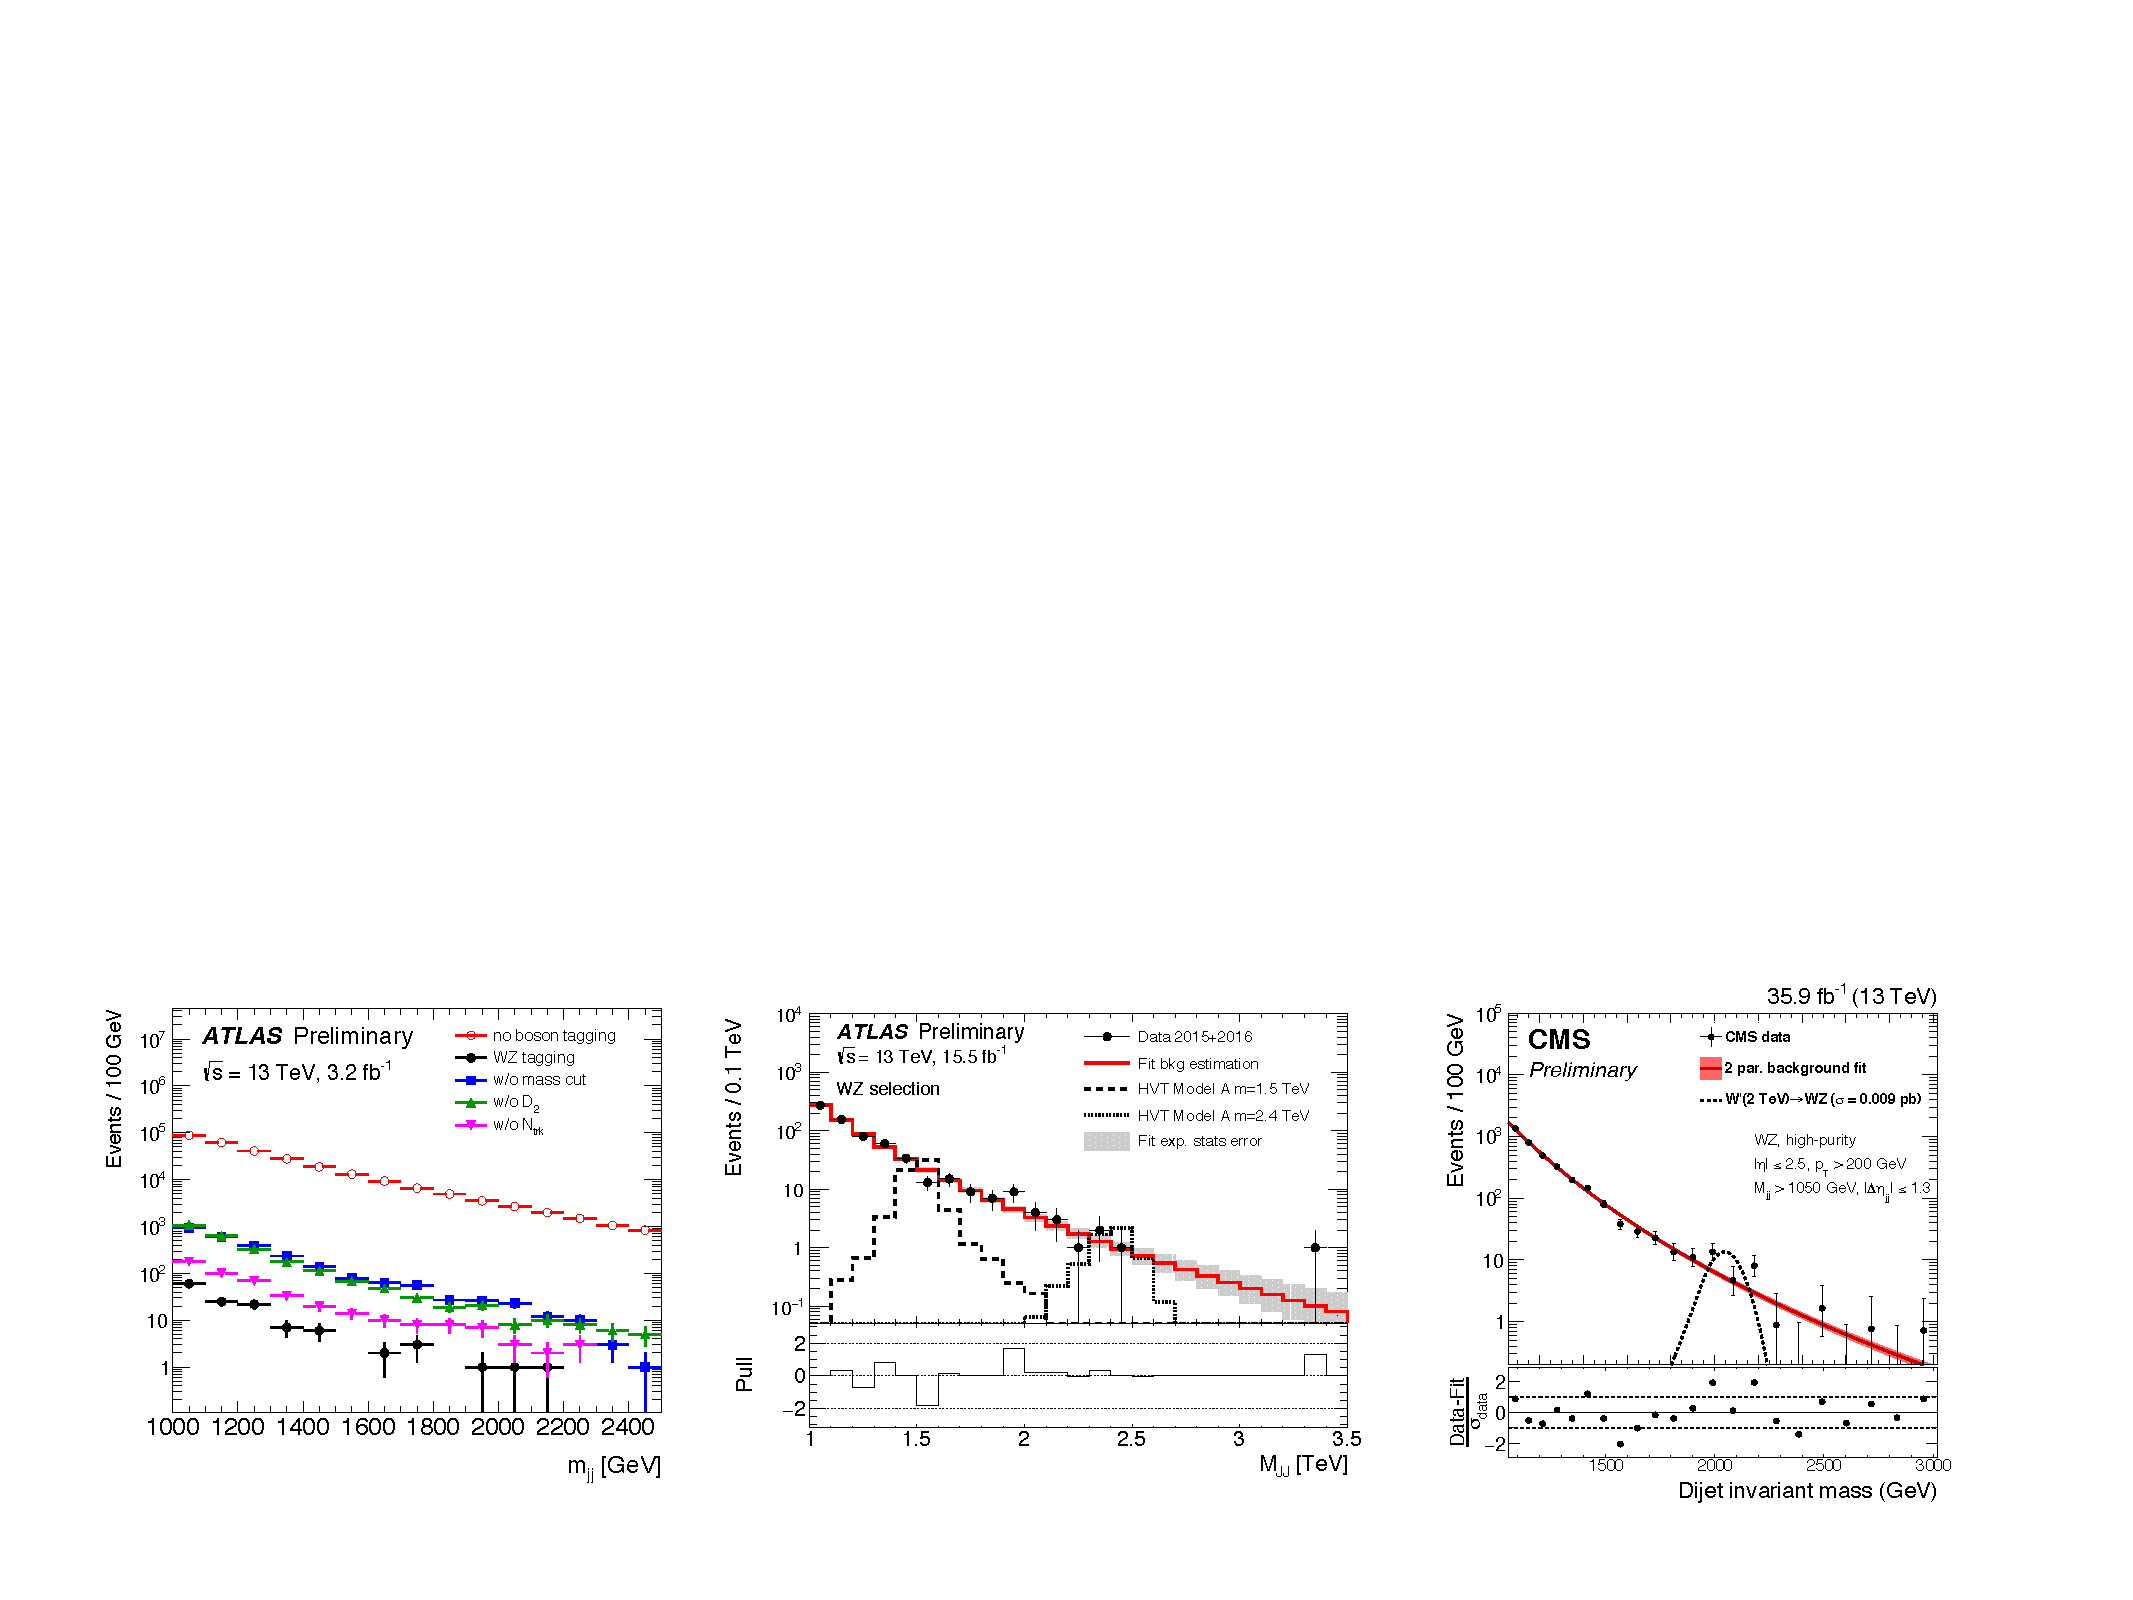
\includegraphics[width=0.99\textwidth]{figures/analysis/search3/misc/bumps1.pdf}\\
    \caption{Several small bumps have been observed in diboson resonance searches in the all-hadronic final state, both in ATLAS and in CMS~\cite{stealth}.}
    \label{fig:searchIII:bumps}
\end{figure}
Due to their small size and the way the excesses appeared to slightly shift around, these were obviously not diboson resonances. However, a proposal was made that they could be caused by the observation of a non-SM boson, such that jets with a mass several standard deviations away from the new particle's mean, its so-called {\it tail}, were being observed, as illustrated in Figure~\ref{fig:searchIII:tails}.
\begin{figure}[h!] 
    \centering
    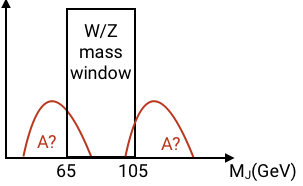
\includegraphics[width=0.3\textwidth]{figures/analysis/search3/misc/tails.png}
    \caption{The small excesses in diboson searches could be caused by the observation of the tail of a non-SM object, peaking at a groomed jet mass slightly higher or lower than that of a W or Z boson.}
    \label{fig:searchIII:tails}
\end{figure}
Further, these could be 4-pronged objects rather than 2-prong, which would cause the excess to vary in size depending on the 4-prong efficiency of the analysis specific W-tagger in use. An explanation for the observed excesses was proposed in~\cite{Aguilar-Saavedra:2018xpl}. This paper pointed out that, if particles like \PWpr and \PZpr exist, an extended scalar sector is needed in order to give mass to the
vector bosons. These heavy scalars would decay to lighter bosons, if kinematically allowed, leading to a cascade of decays that produced signals of multiple bosons in a single jet. Some example signatures are illustrated in Figure~\ref{fig:searchIII:tribosons}.
\begin{figure}[h!] 
    \centering
    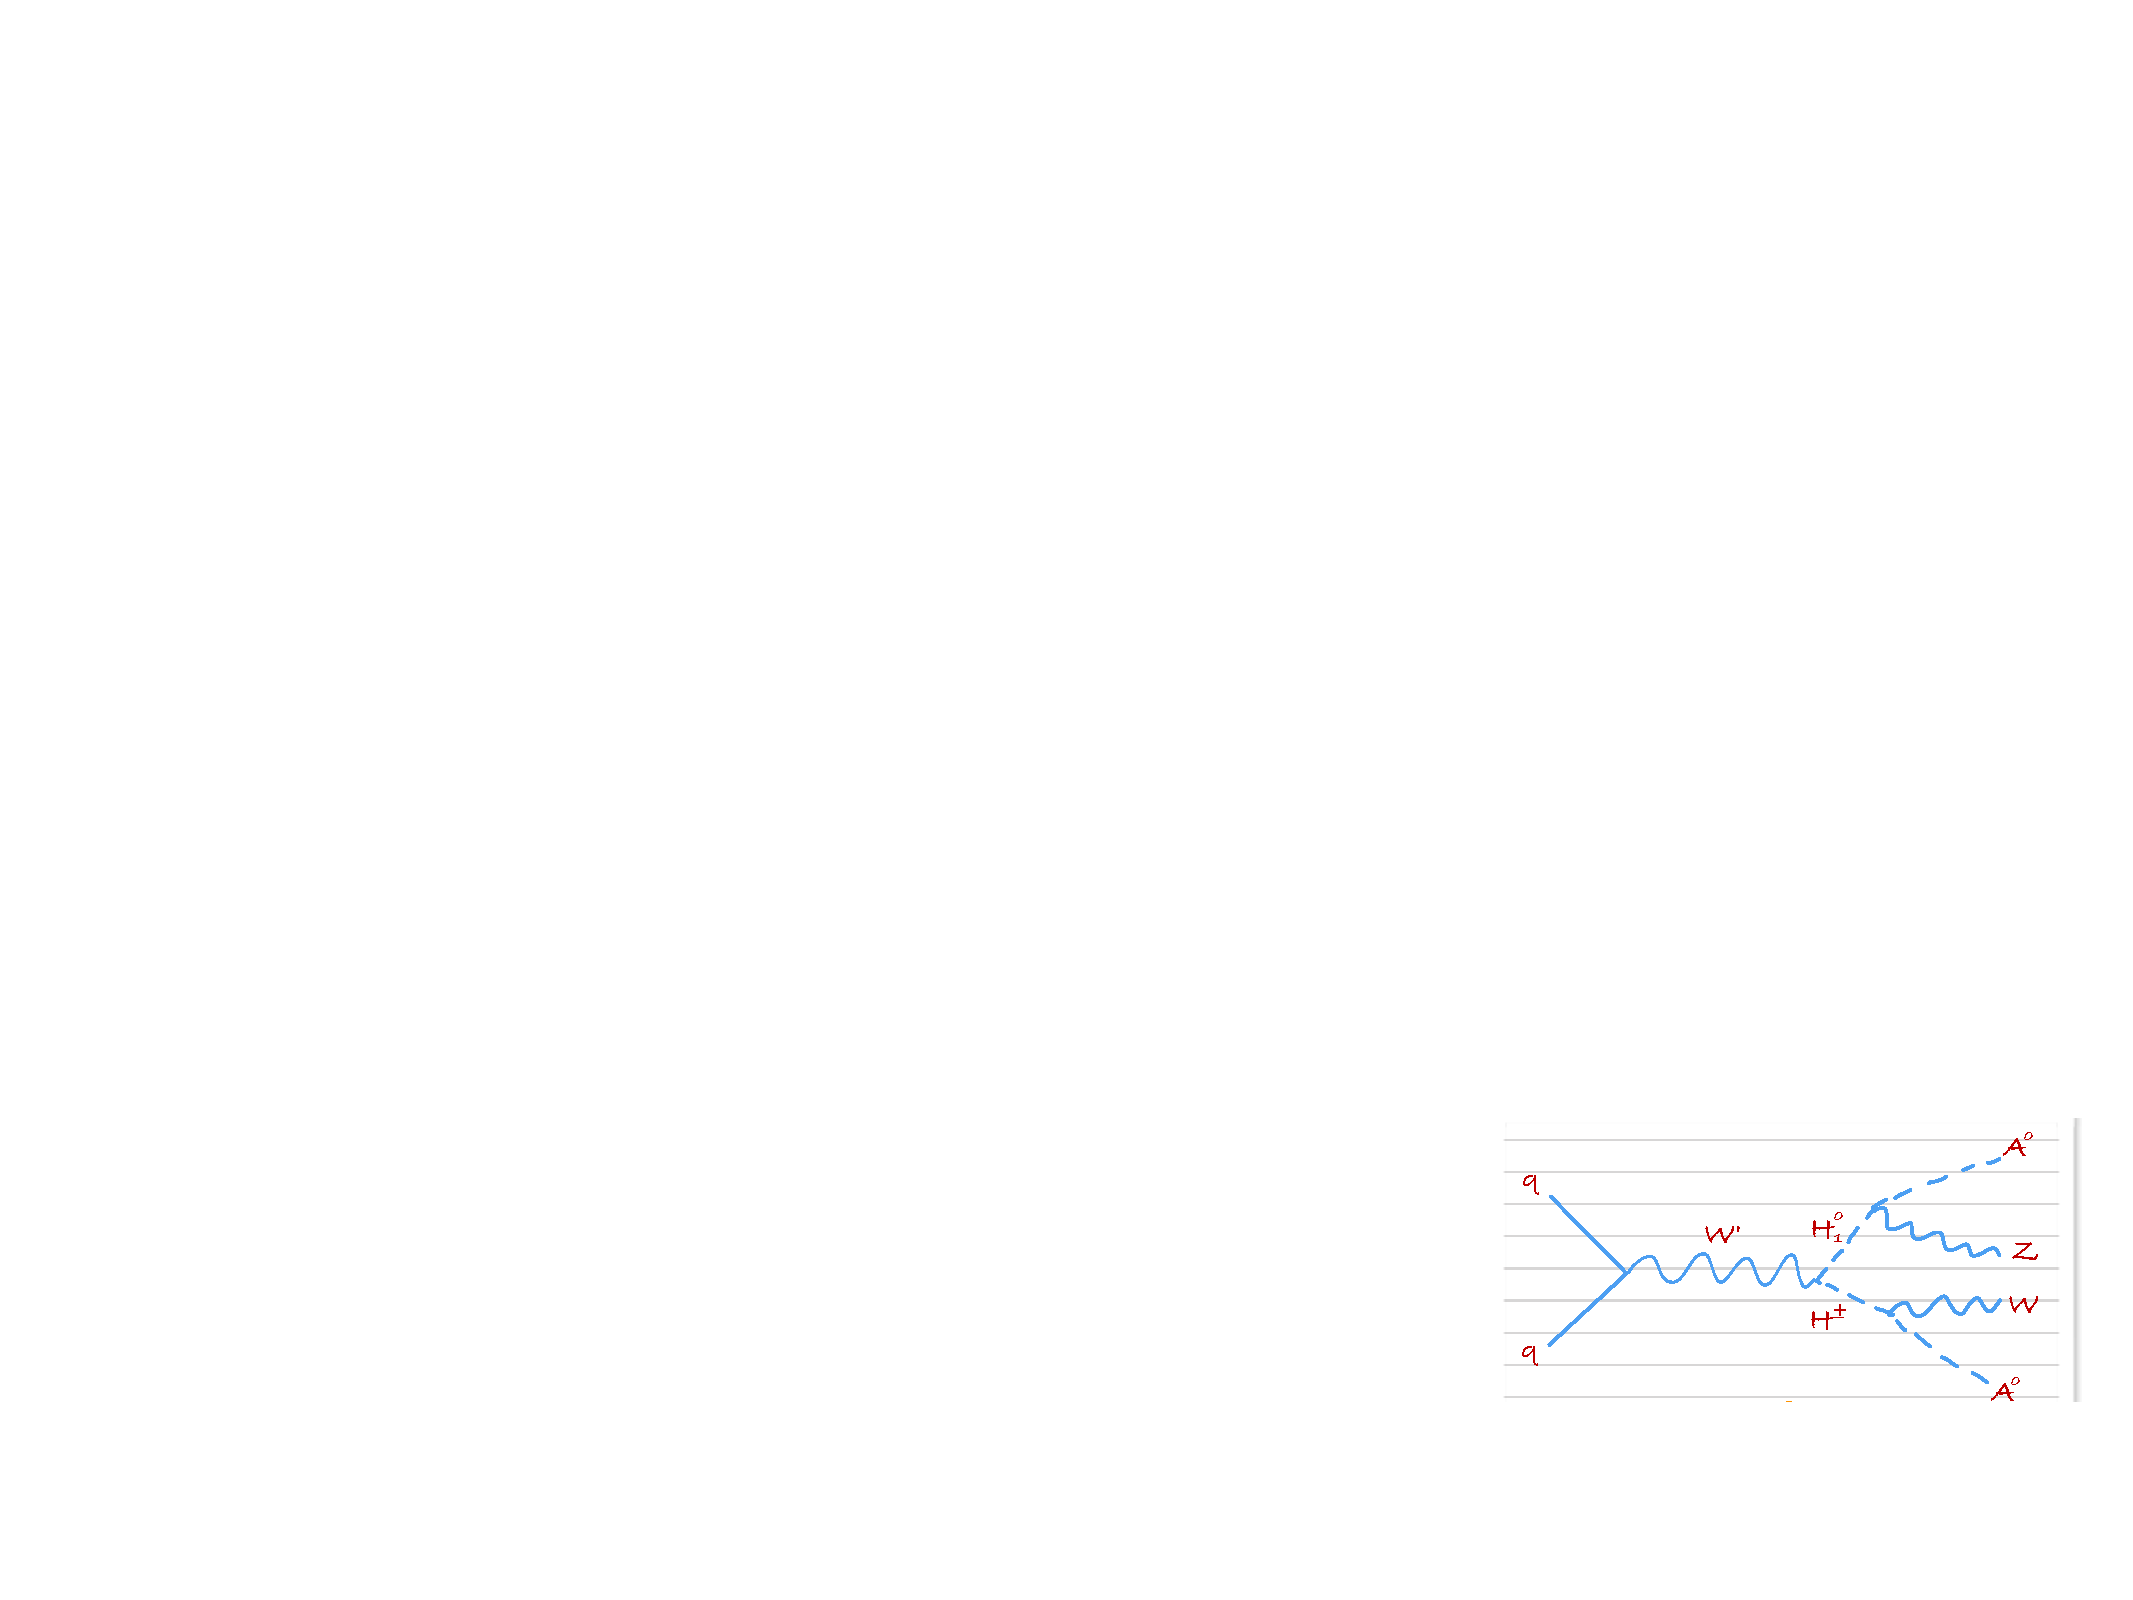
\includegraphics[height=3cm]{figures/analysis/search3/misc/quadri.pdf}
    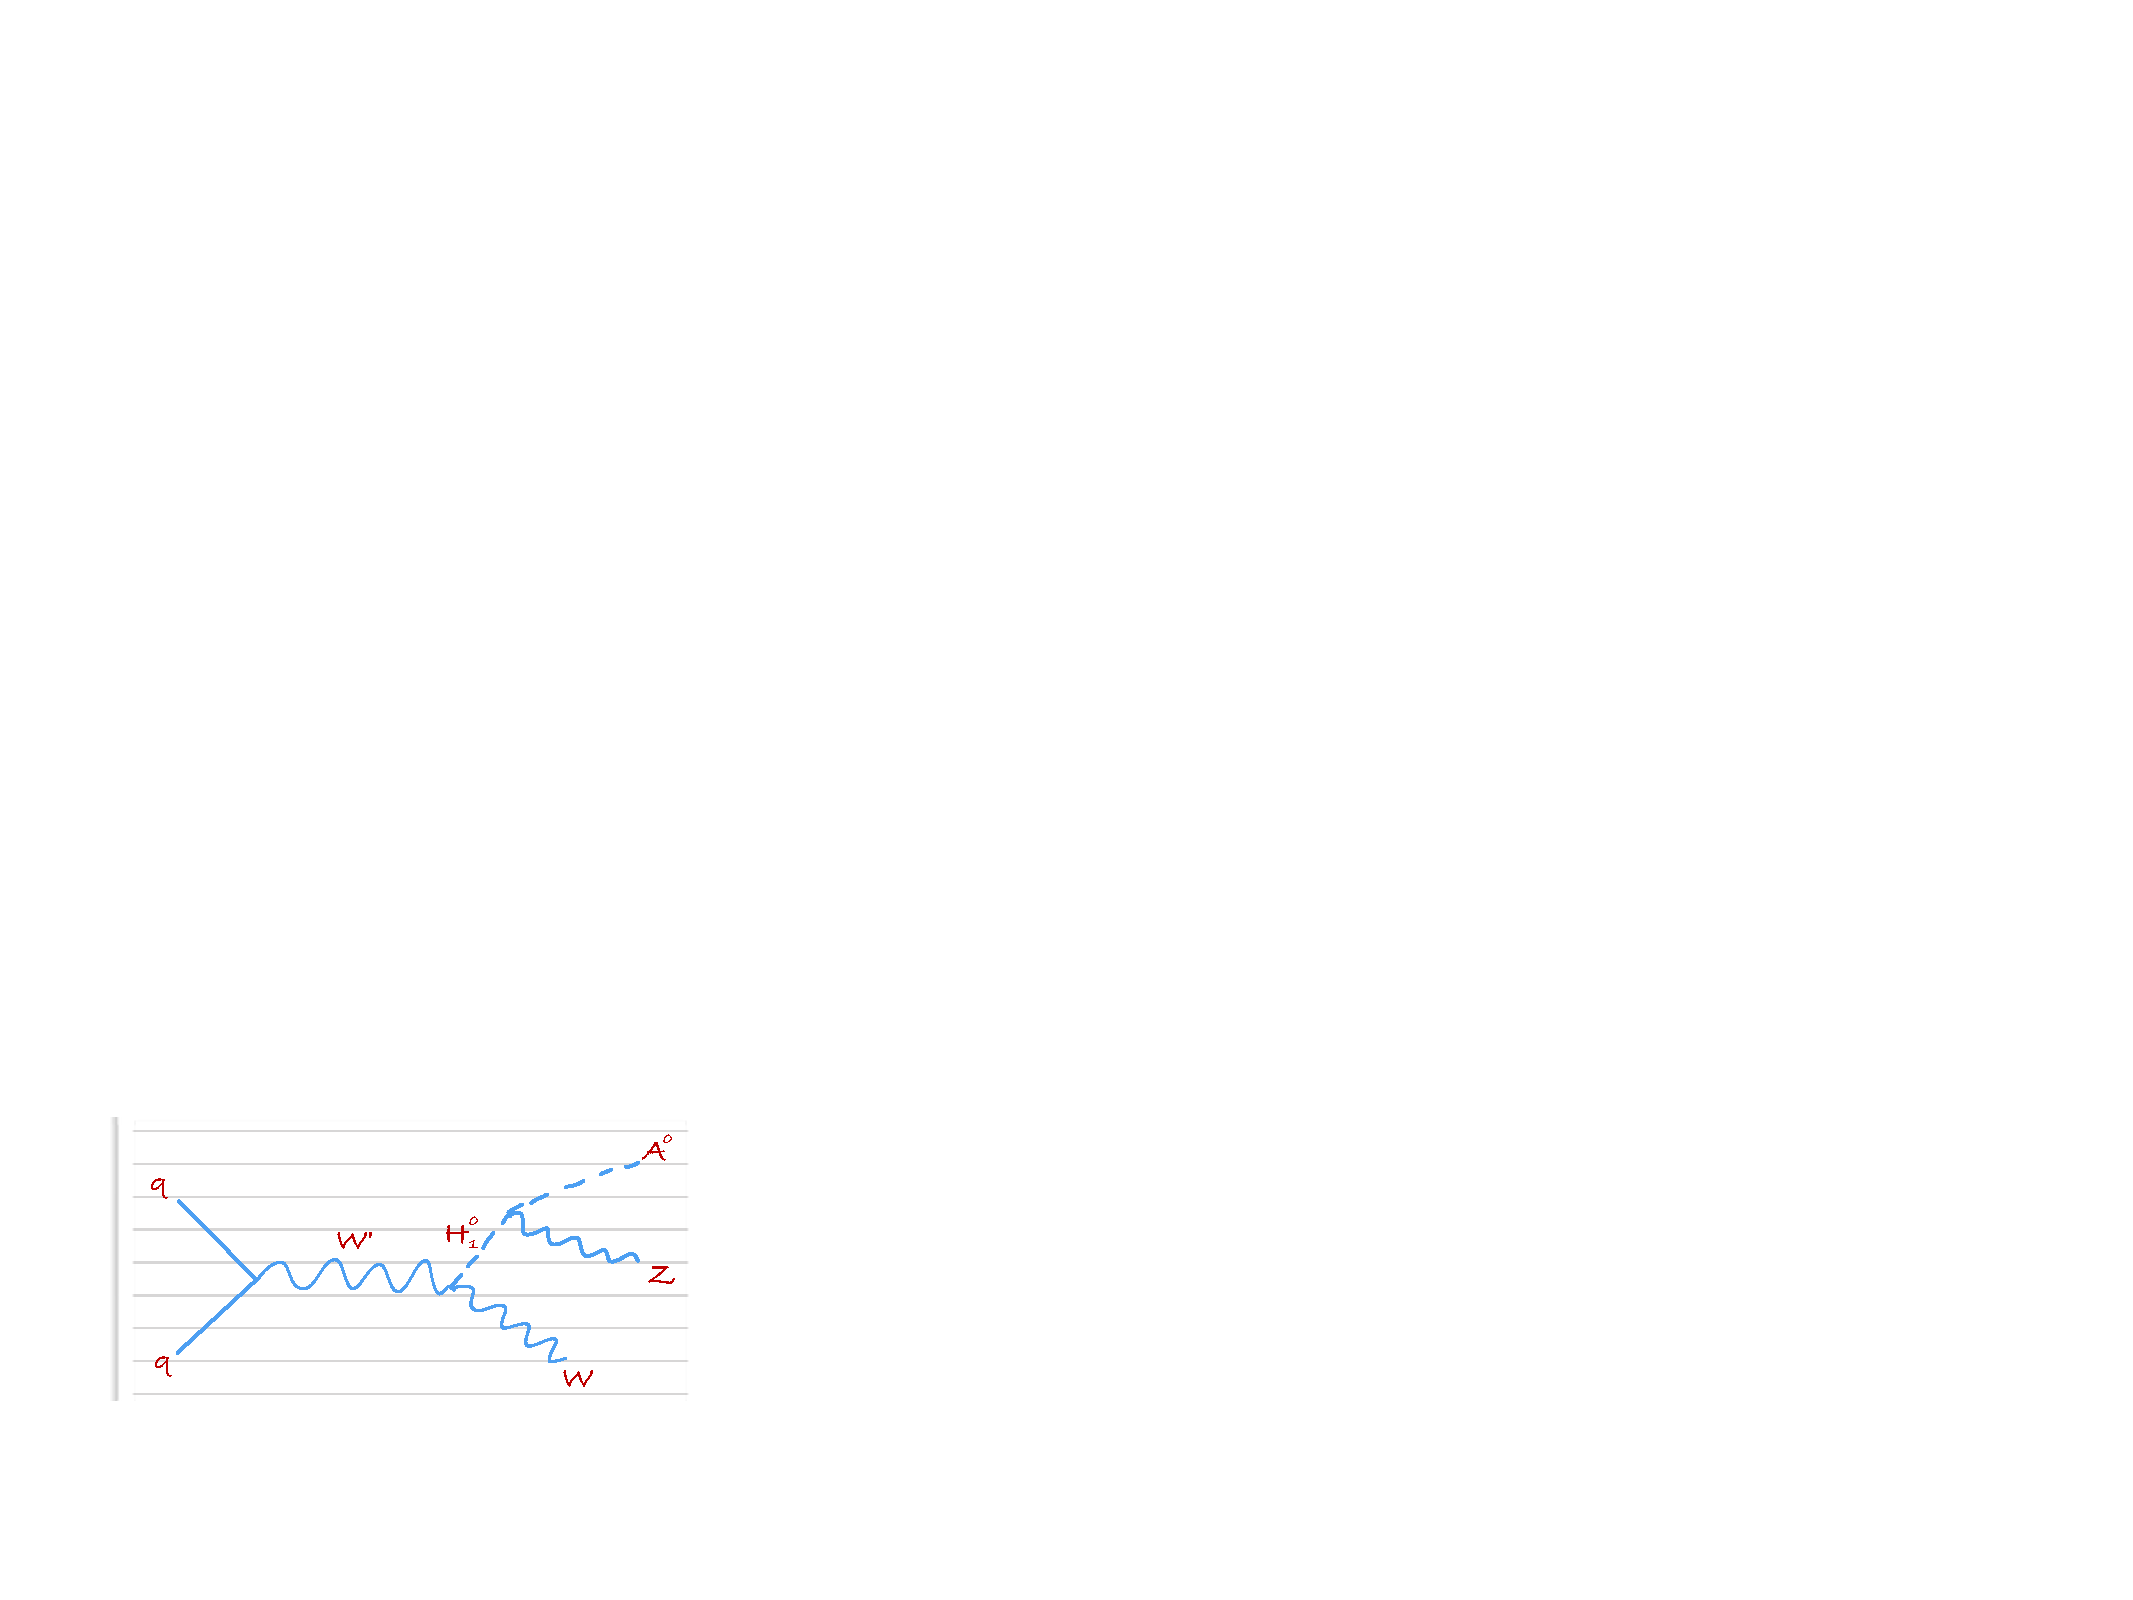
\includegraphics[height=3cm]{figures/analysis/search3/misc/tri1.pdf}
    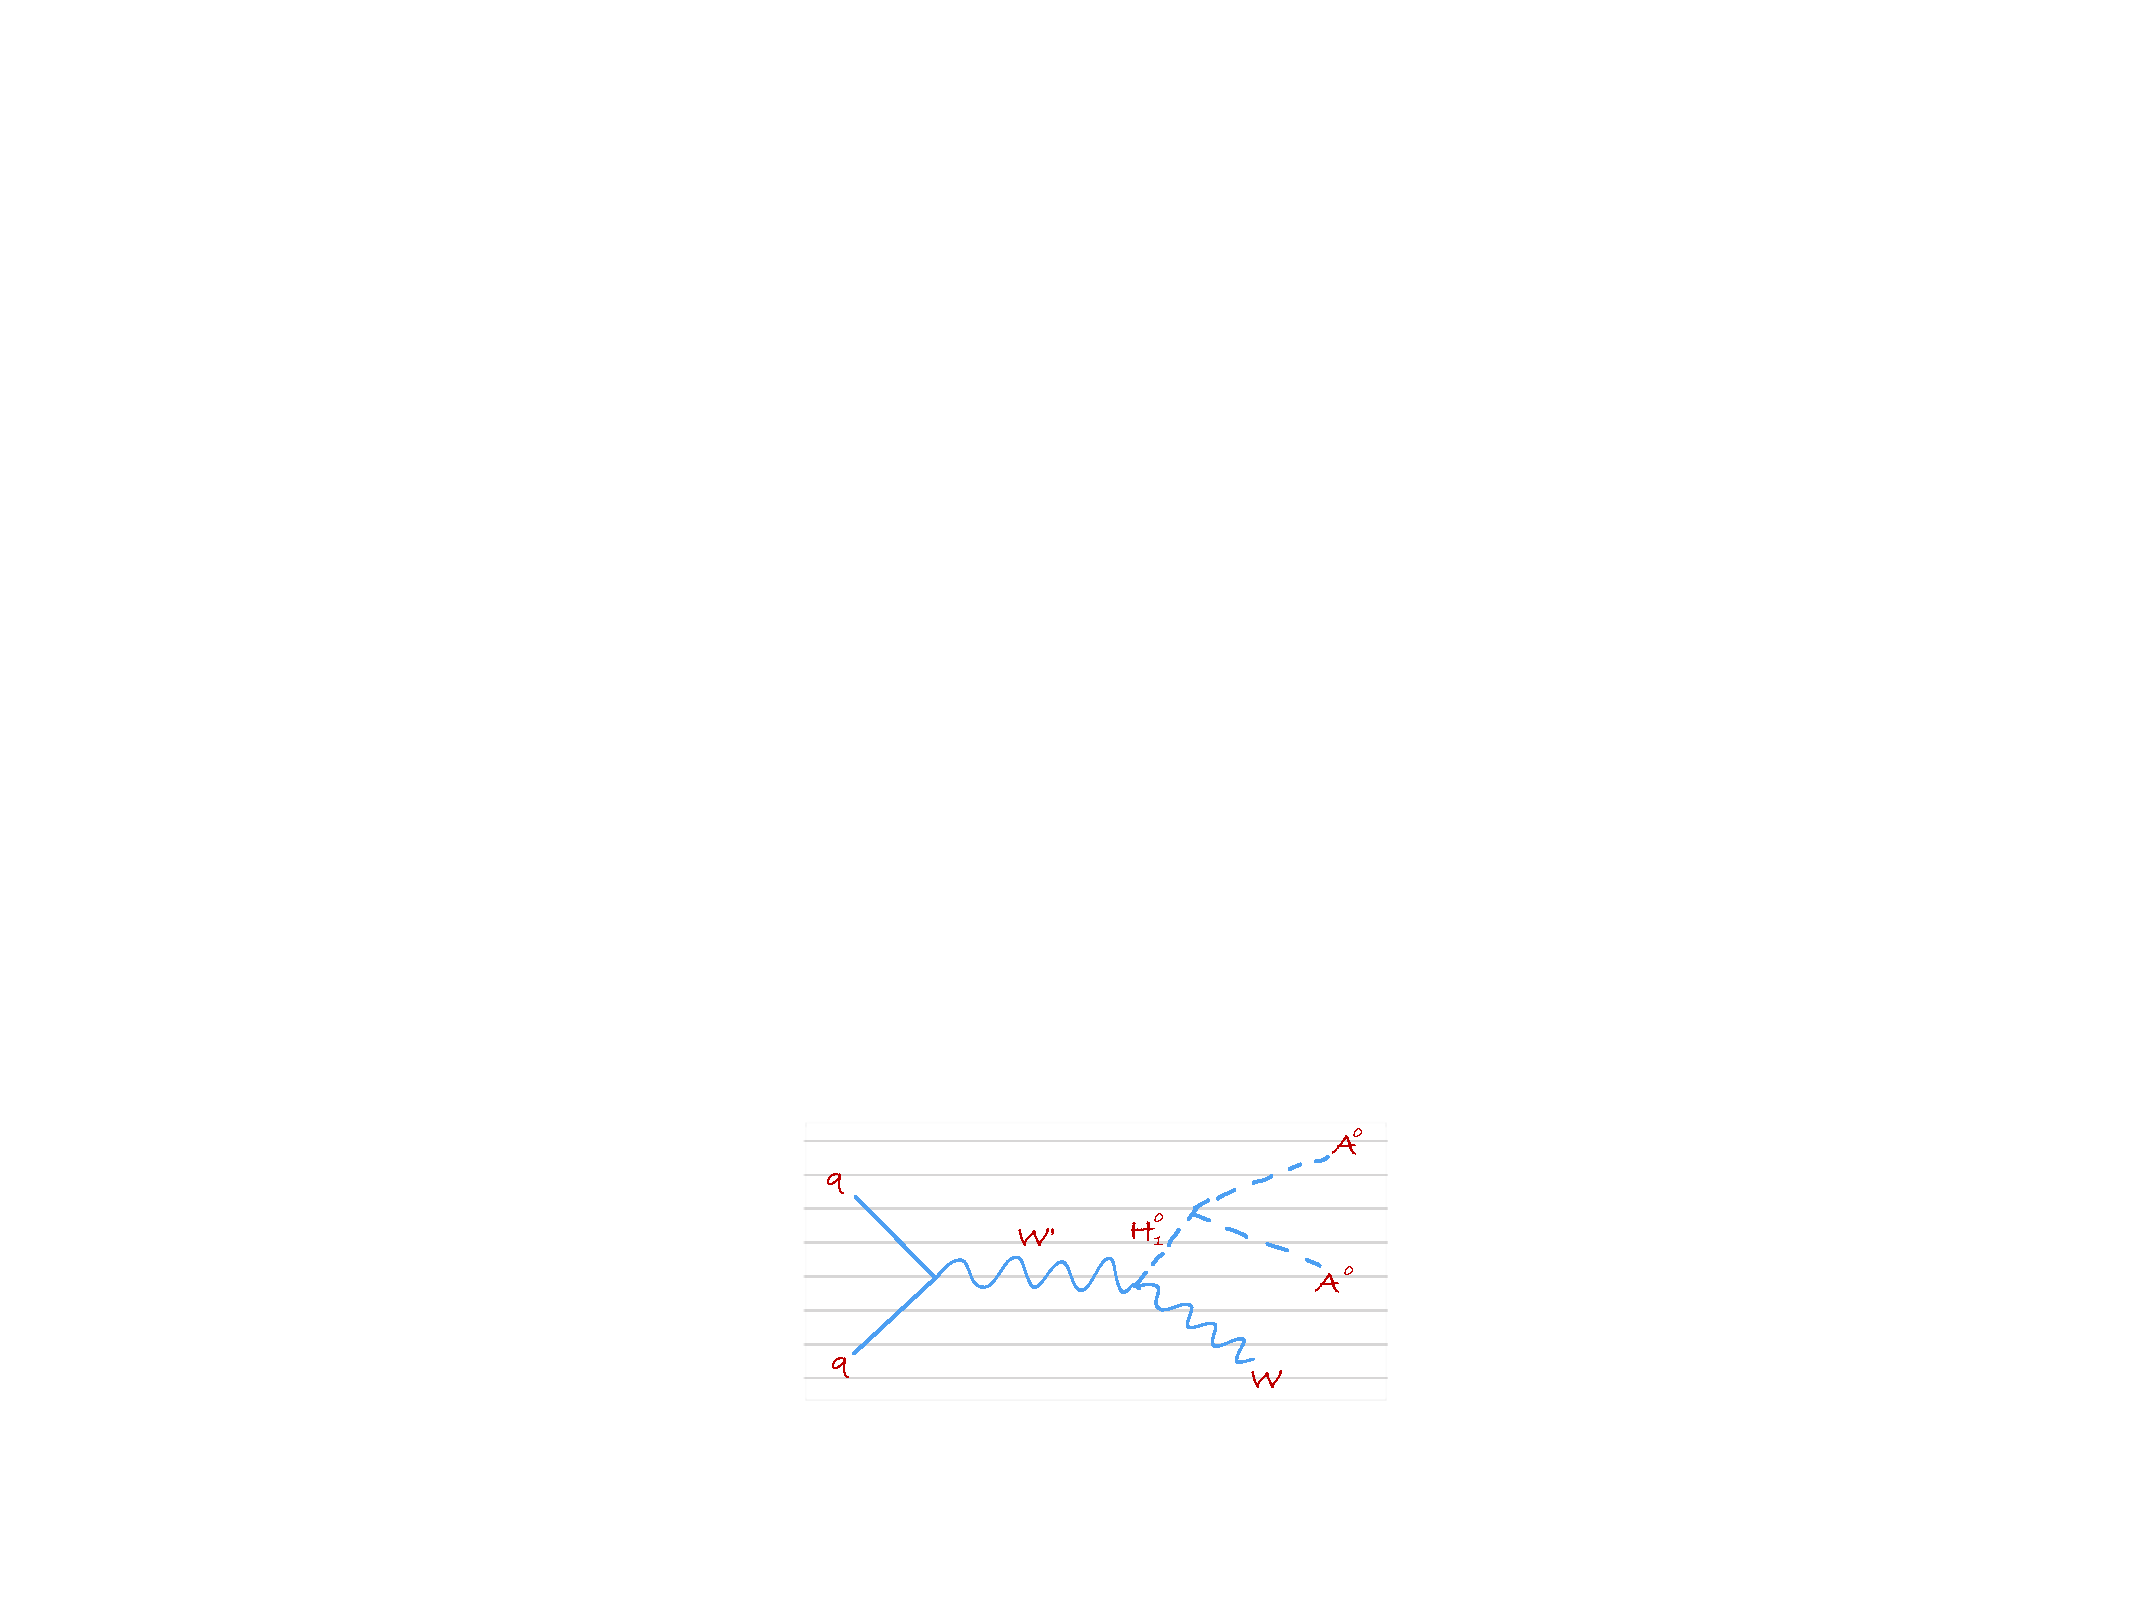
\includegraphics[height=3cm]{figures/analysis/search3/misc/tri2.pdf}
    \caption{A \PWpr decaying to a neutral $\rm{H}^0$ and a charged $\rm{H}^{\pm}$ scalar particle leading to a quadriboson final state (left), and a \PWpr decaying to a neutral scalar particle $\rm{H}^0$ and a \PW leading to a triboson final state (middle and right)~\cite{Aguilar-Saavedra:2018xpl}.}
    \label{fig:searchIII:tribosons}
\end{figure}
Signatures like these would peak in the groomed-jet mass spectrum and, depending on what the final bosons decay into, have very different substructure profiles.\par
In order to efficiently search for such types of signals, or any signal peaking in the jet mass spectrum, we decided to build a generic framework that would allow searching for peaks anywhere in the jet-mass and dijet invariant mass spectrum.
Rather than selecting jets with a groomed mass between 65 and 105 \GeV and then searching for resonances peaking in the dijet invariant mass, we would attempt to look for resonances peaking anywhere in the three-dimensional space formed by the groomed mass of each jet and their dijet invariant mass, scanning the full groomed mass spectrum in a single analysis. We would first demonstrate the new method in context of the diboson all-hadronic search since this was an analysis we were familiar with and which would allow for a straight forward comparison of the obtained results.
\section{Analysis strategy}
The background estimation used in Search I and Search II relies on a one-dimensional fit of the dijet invariant mass of the signal region after a tight selection on the jet mass has been applied. Since the signal will peak in all three dimensions, mainly the dijet invariant mass $\MVV$, and the mass of jet 1 and jet 2 ($\MJO$ and $\MJT$), we will extract the signal from the three-dimensional plane of $\MVV$-$\MJO$-$\MJT$.
\begin{figure}[h!] 
    \centering
    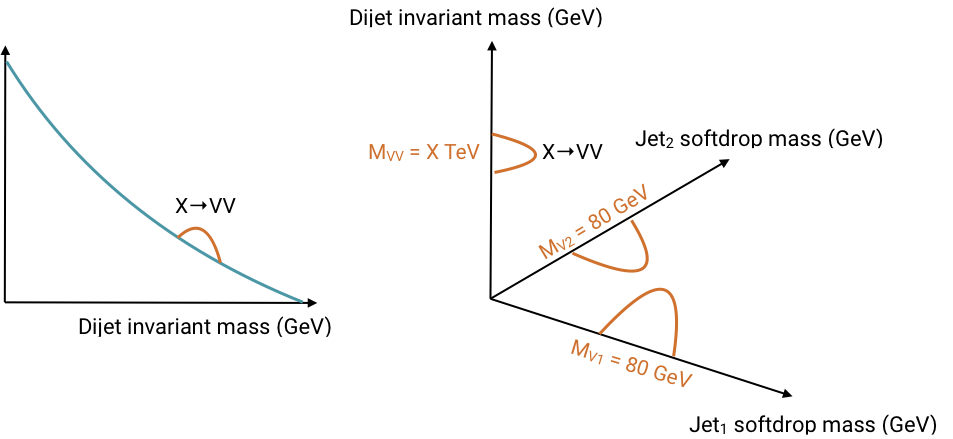
\includegraphics[width=0.79\textwidth]{figures/analysis/search3/misc/1Dvs3D.png}
    \caption{The one dimensional diboson analysis versus the three dimensional fit.}
    \label{fig:searchIII:1Dvs3D}
\end{figure}
The benefits of doing so are that we can search for resonances decaying to VV (V=W/Z), VH (H=Higgs), HH, VX, VH, XX, or XY, where X and Y are new hypothetical bosons, in the same analysis. Additionally, a jet-mass selection is no longer needed as we fit the full jet mass line-shape to extract the signal. This effectively increases the signal statistics since a large fraction of the W and Z signal falls outside the mass window. Fitting the groomed-jet mass and resonance mass together also allows for the addition of nuisance parameters that simultaneously affect both in order to fully account for the correlation between the variables. Finally, we would model the background starting from simulation, rather than from a dijet fit to data. This allows the background shape to assume non-smooth distributions, and could allow the search to probe lower dijet masses, something we will discuss further in Section~\ref{sec:searchIII:trigger}. Replacing the parametric fit by a simulation-based model would also reduce the fit sensitivity to background fluctuations in the extreme tails of the dijet invariant mass spectrum. \par
This chapter presents a novel three-dimensional fit method in the search for diboson resonances in the all-hadronic final state, and is based on 77.3 \fbinv of data collected in 2016 and 2017. The data collected in 2016 was already analyzed in the context of Search II, but is reanalyzed here in order to compare the performance of the three-dimensional fit to that of the one dimensional search.

\section{Data and simulated samples}
The data analyzed in this search consists of 35.9 \fbinv of data collected in 2016 and 41.4 \fbinv of data collected in 2017, yielding a total of 77.3 \fbinv.\newline
The simulated samples are the same as those described in Section~\ref{sec:searchII:samples}.

\section{Event selection}
Events are selected following the same criteria as in Search I and Search II (see Section~\ref{sec:searchI:preselection}) and can be summarized as follows: we require two AK8 jets with PUPPI pileup subtraction applied, and with $\eta < 2.5$ and \pt $> 200$ GeV. The two jets are further required to be separated by $|\Delta\eta|_{jj} < 1.3$. The softdrop algorithm is applied, and the two jets with the highest jet mass in the event are selected as potential vector boson candidates. In order to avoid any bias in the jet mass shapes when performing the three-dimensional fit, the two jets are randomly sorted after the above selections have been applied. In addition, the dijet invariant mass is required to be greater than 1126 GeV in order to be on the trigger plateau. As already mentioned in the introduction, the background modeling used in this analysis is capable of modeling trigger turn-ons. We explored the possibility of starting the analysis below the trigger plateau, however, while the background modeling was found to be reliable, the extraction of a signal peaking on top of a turn-on was difficult, and we therefore had to abandon the modeling of the trigger turn-on for this first demonstration of the method. More details will be given in Section~\ref{sec:searchIII:trigger}. The dijet invariant mass and $|\Delta\eta|_{jj}$ distribution for the two leading jets in the event after the above preselections have been applied are shown in Figure~\ref{fig:Mjj-all} and the jet \PT{} and $\eta$ distributions for signal and for background is shown in Figure~\ref{fig:kinematics-all}.
\begin{figure}[h!]
\centering
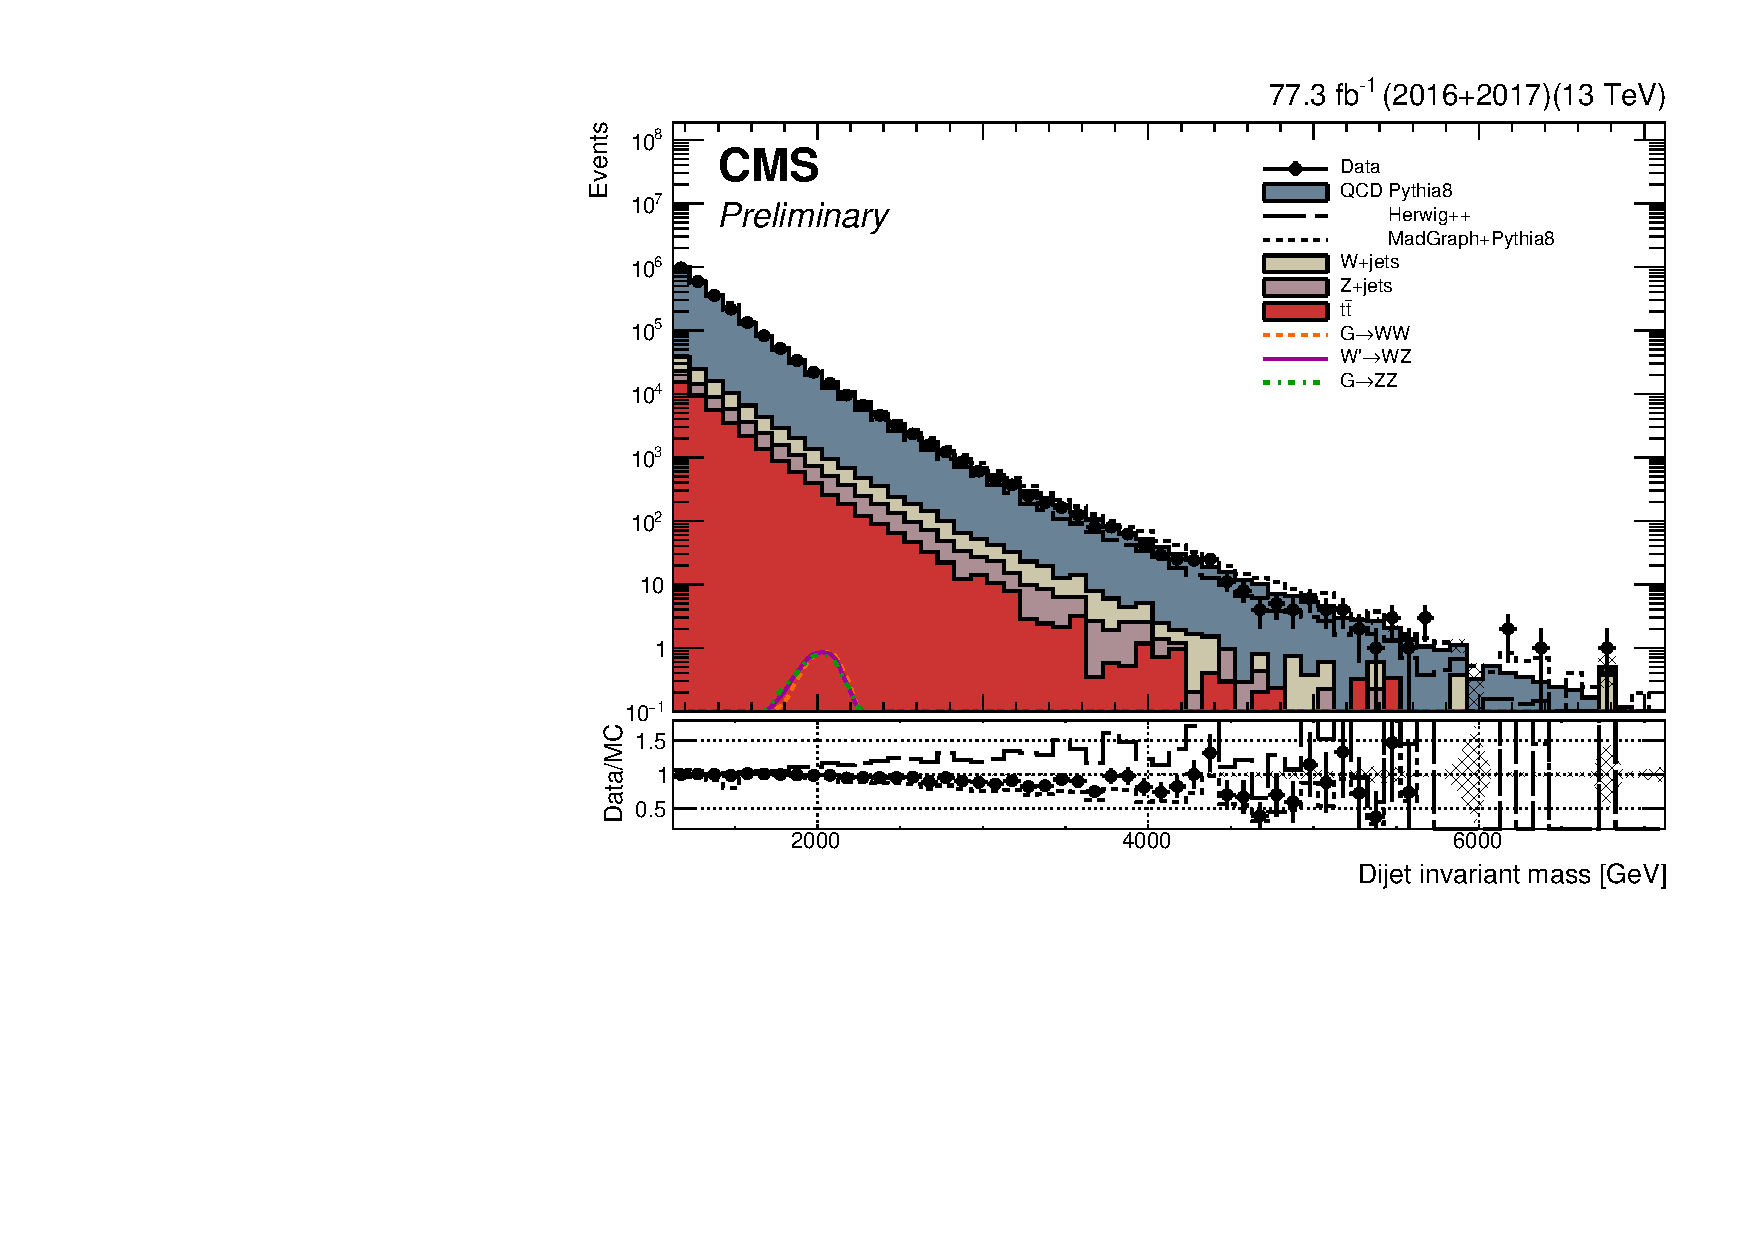
\includegraphics[width=0.450\textwidth]{figures/analysis/search3/AN-17-303/controlPlots/looseSel_Dijet_invariant_mass.pdf}
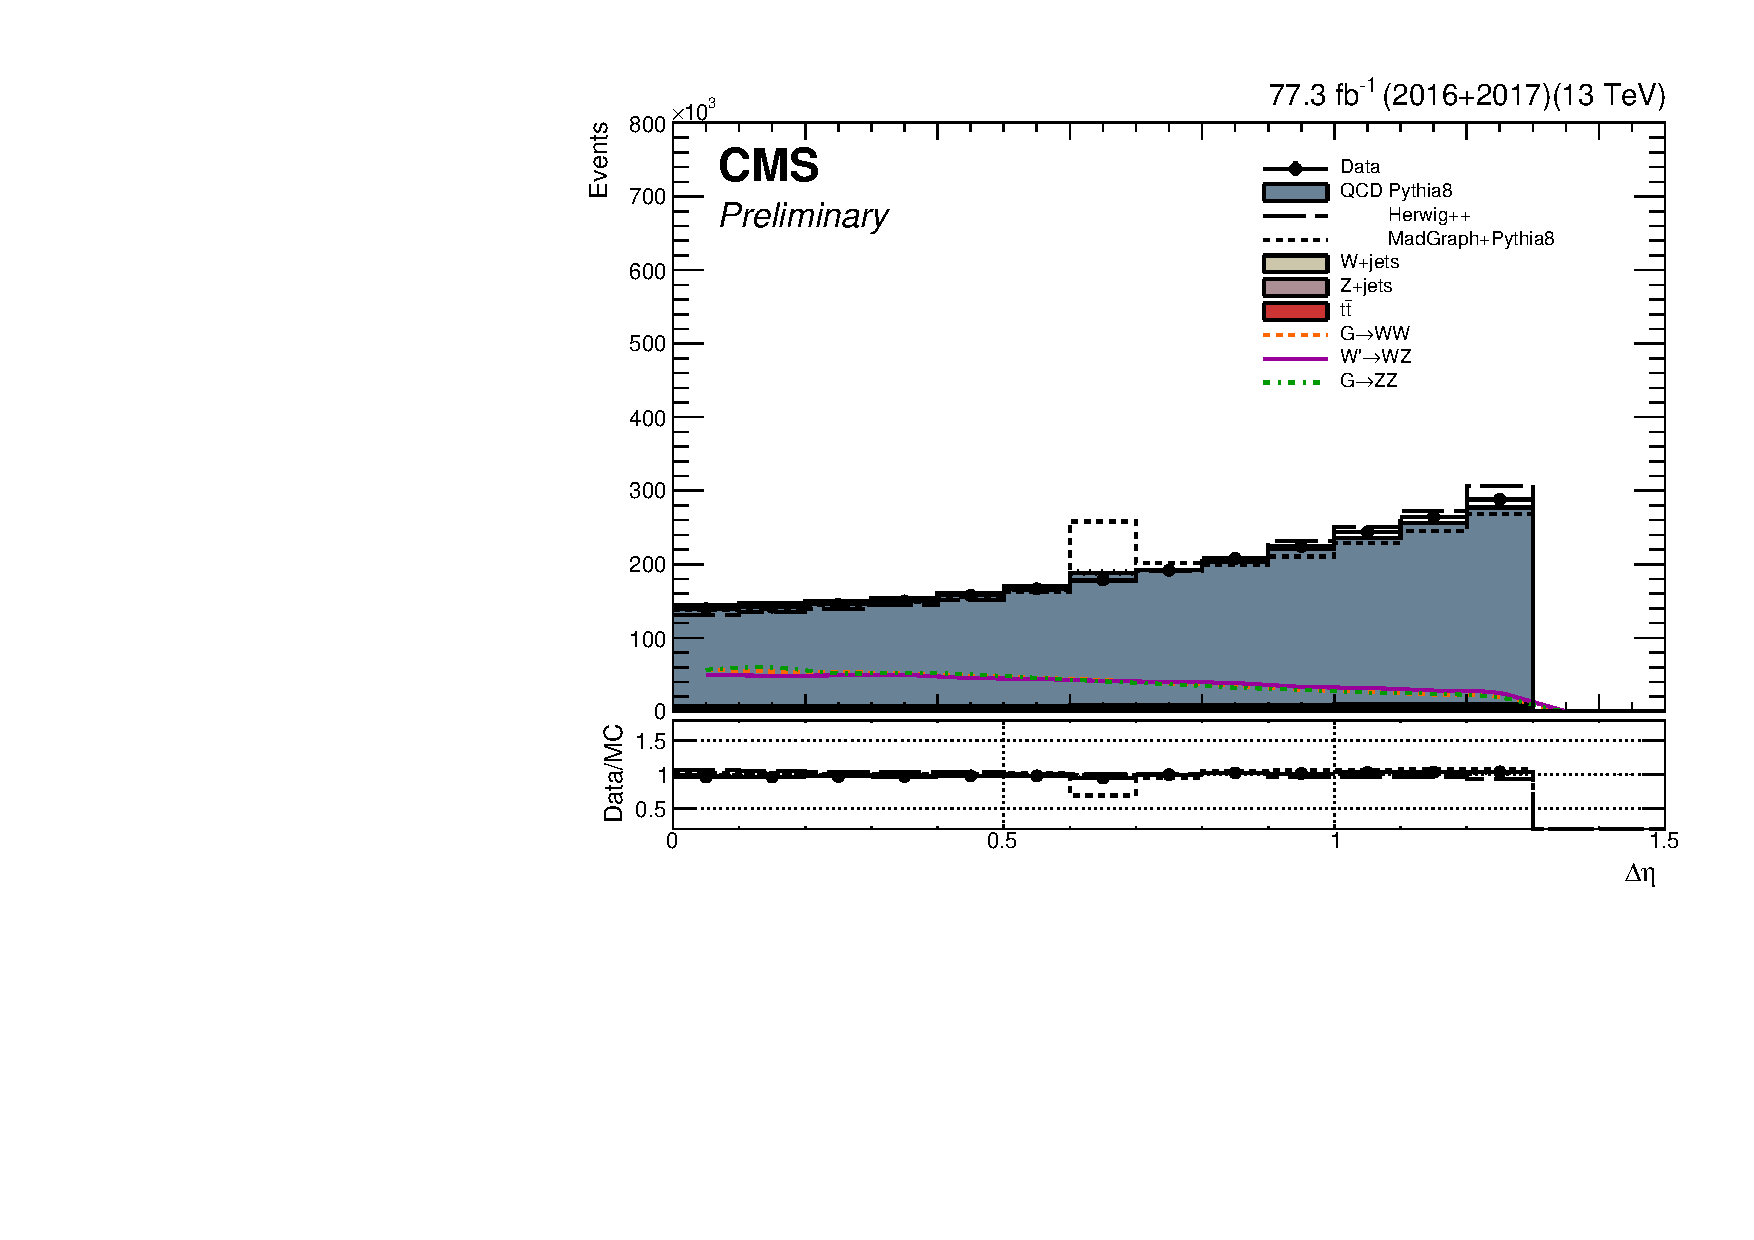
\includegraphics[width=0.450\textwidth]{figures/analysis/search3/AN-17-303/controlPlots/looseSel_Deltaeta.pdf}
\caption{The dijet invariant mass (left) and $|\Delta\eta|_{jj}$ (right) for the two leading jets after preselections are applied. The signal is scaled by an arbitrary number to be visible.}
\label{fig:Mjj-all}
\end{figure}
\begin{figure}[h!]
\centering
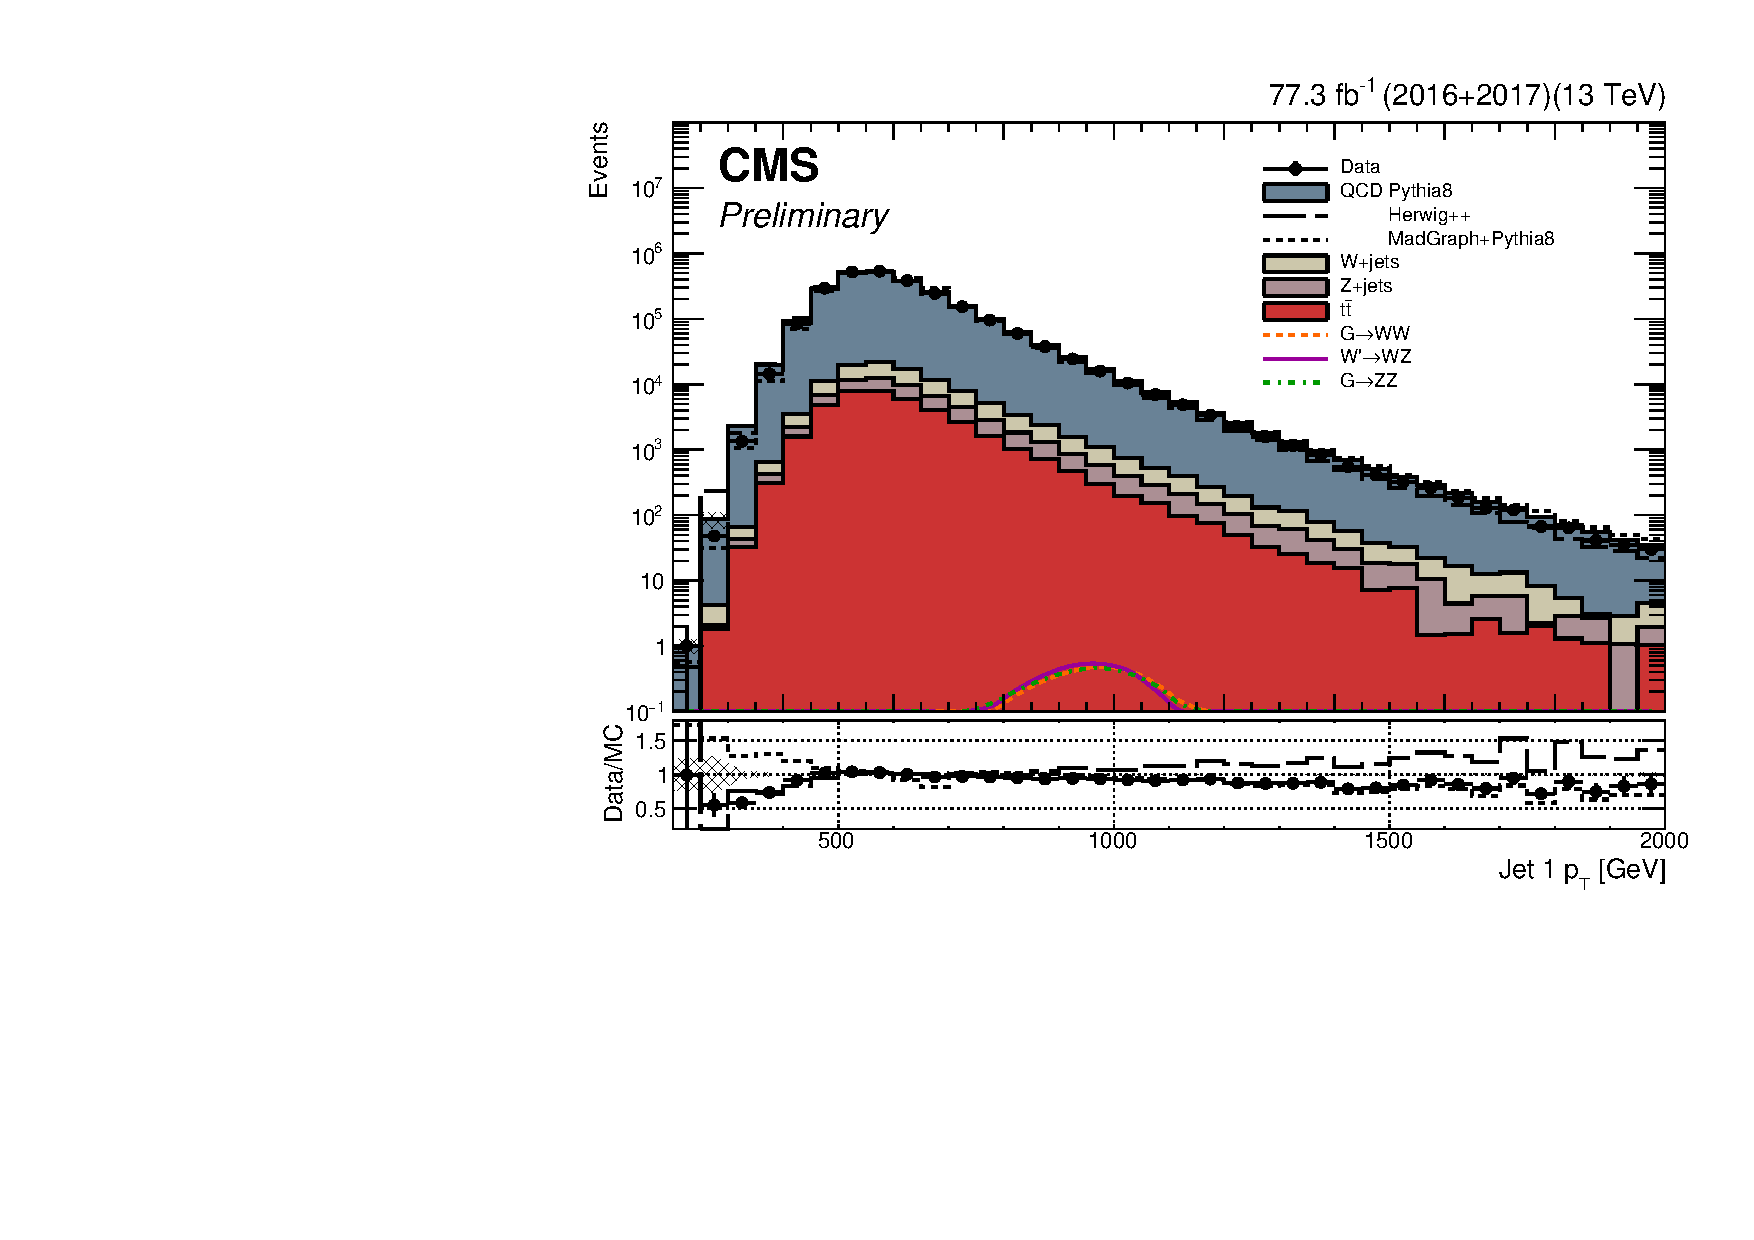
\includegraphics[width=0.450\textwidth]{figures/analysis/search3/AN-17-303/controlPlots/looseSel_Jet_1_p_T.pdf}
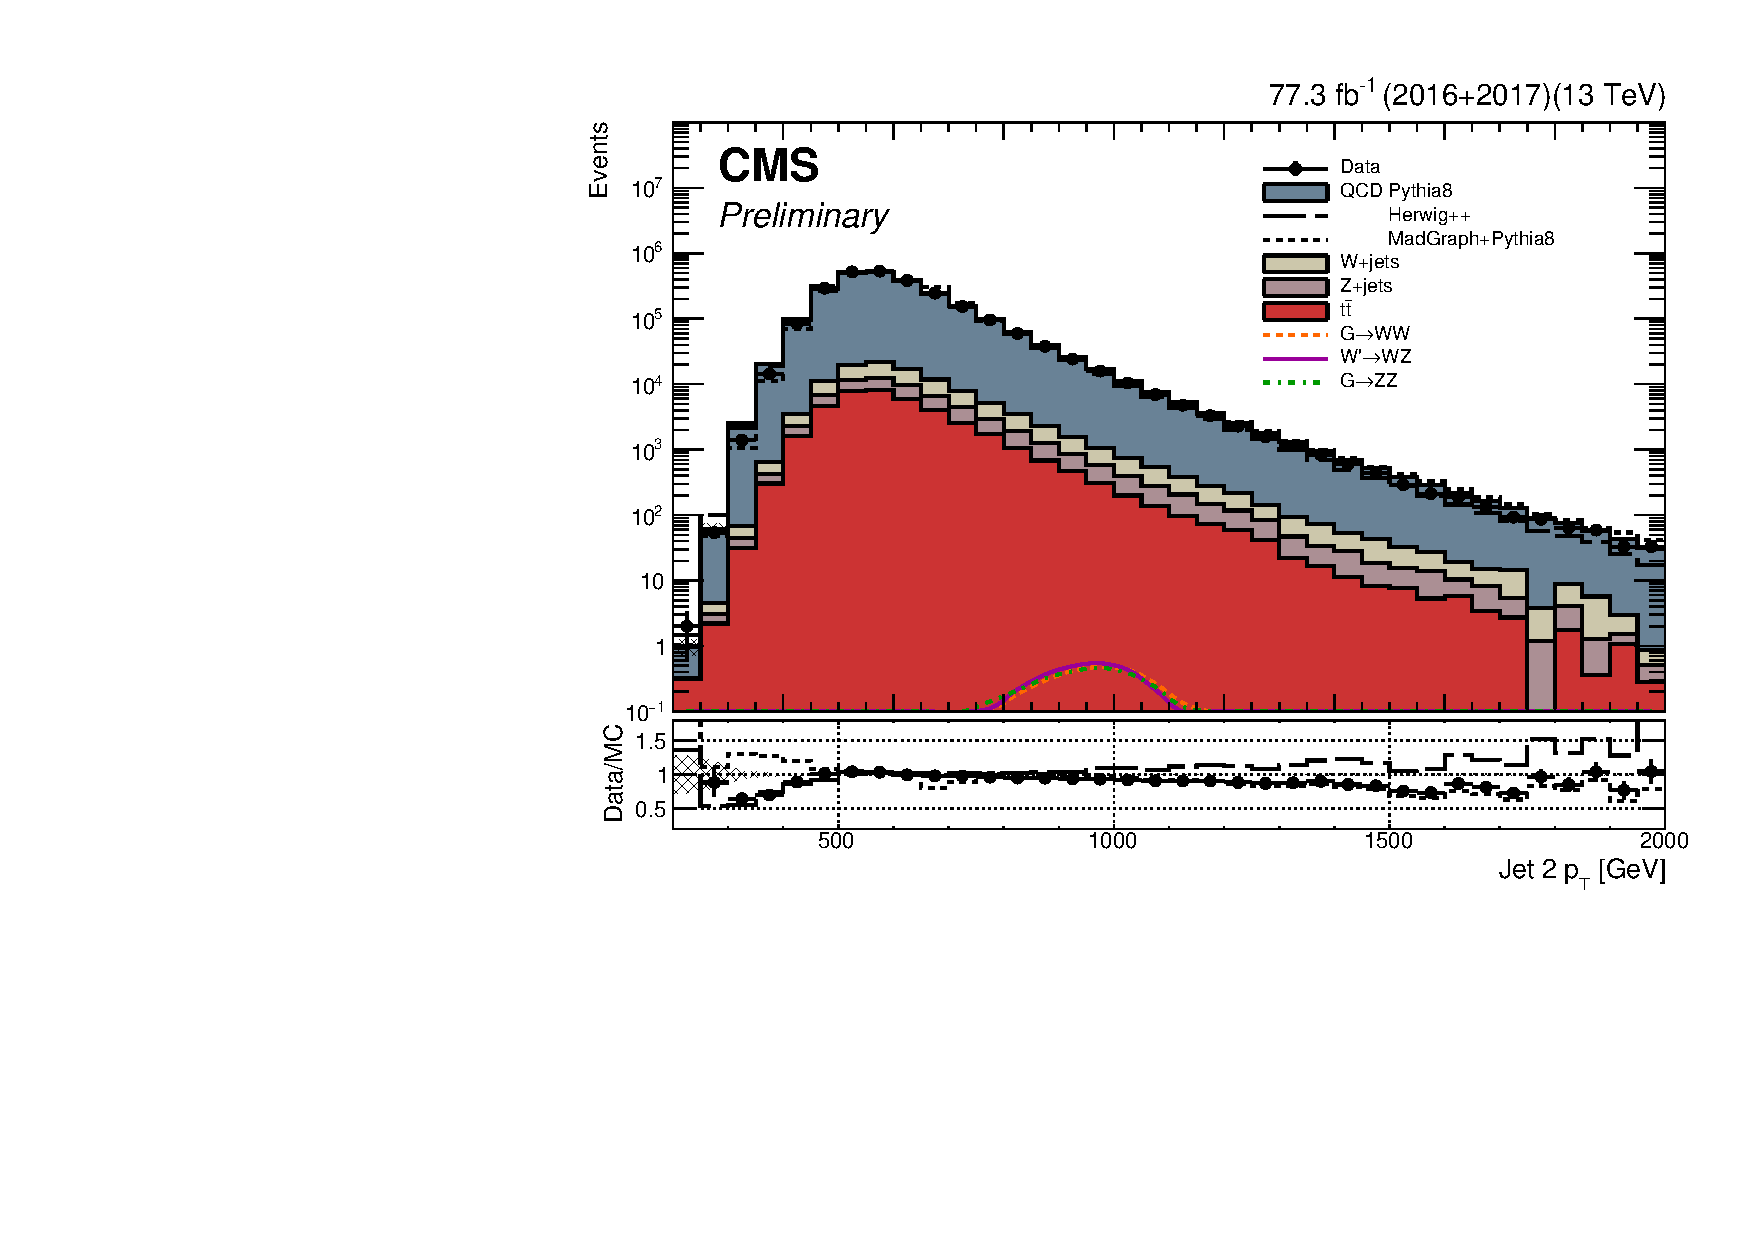
\includegraphics[width=0.450\textwidth]{figures/analysis/search3/AN-17-303/controlPlots/looseSel_Jet_2_p_T.pdf}\\
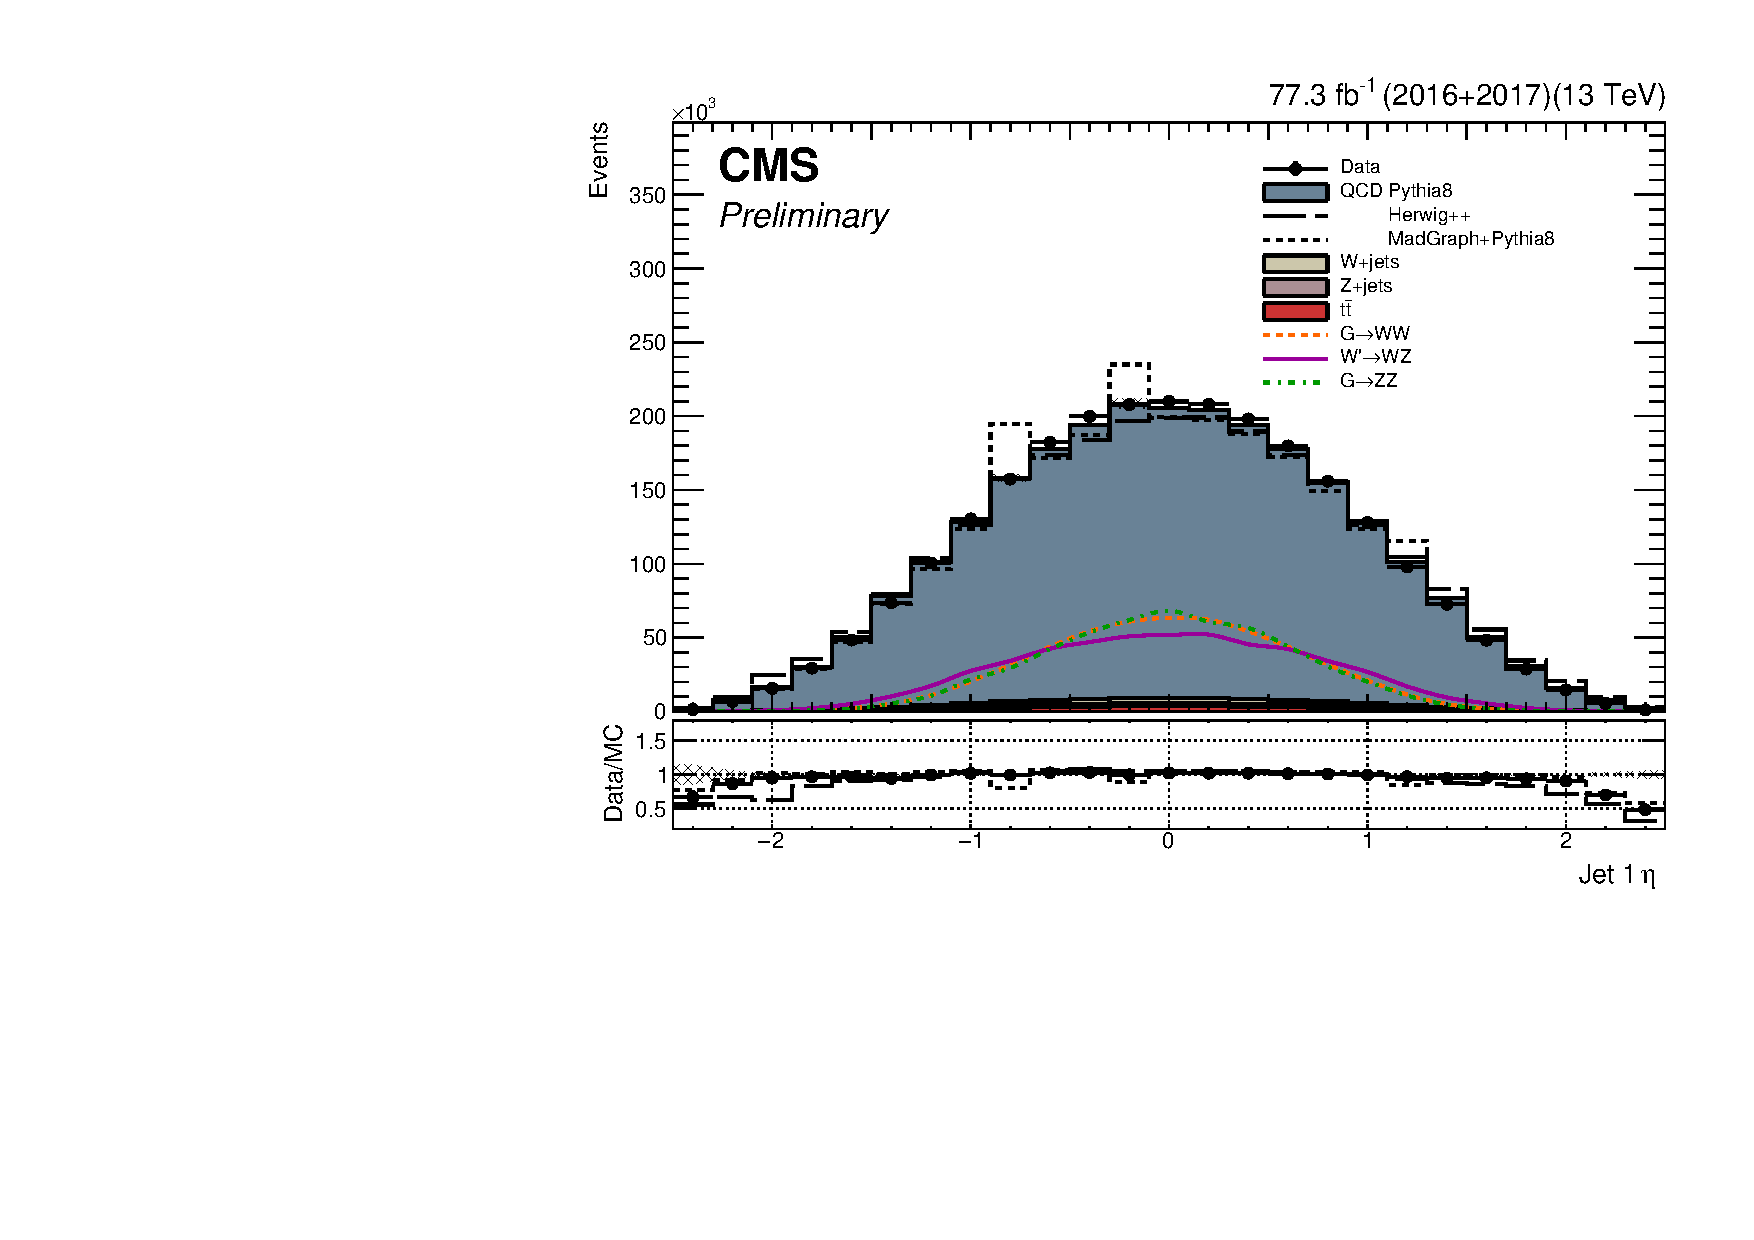
\includegraphics[width=0.450\textwidth]{figures/analysis/search3/AN-17-303/controlPlots/looseSel_Jet_1_eta.pdf}
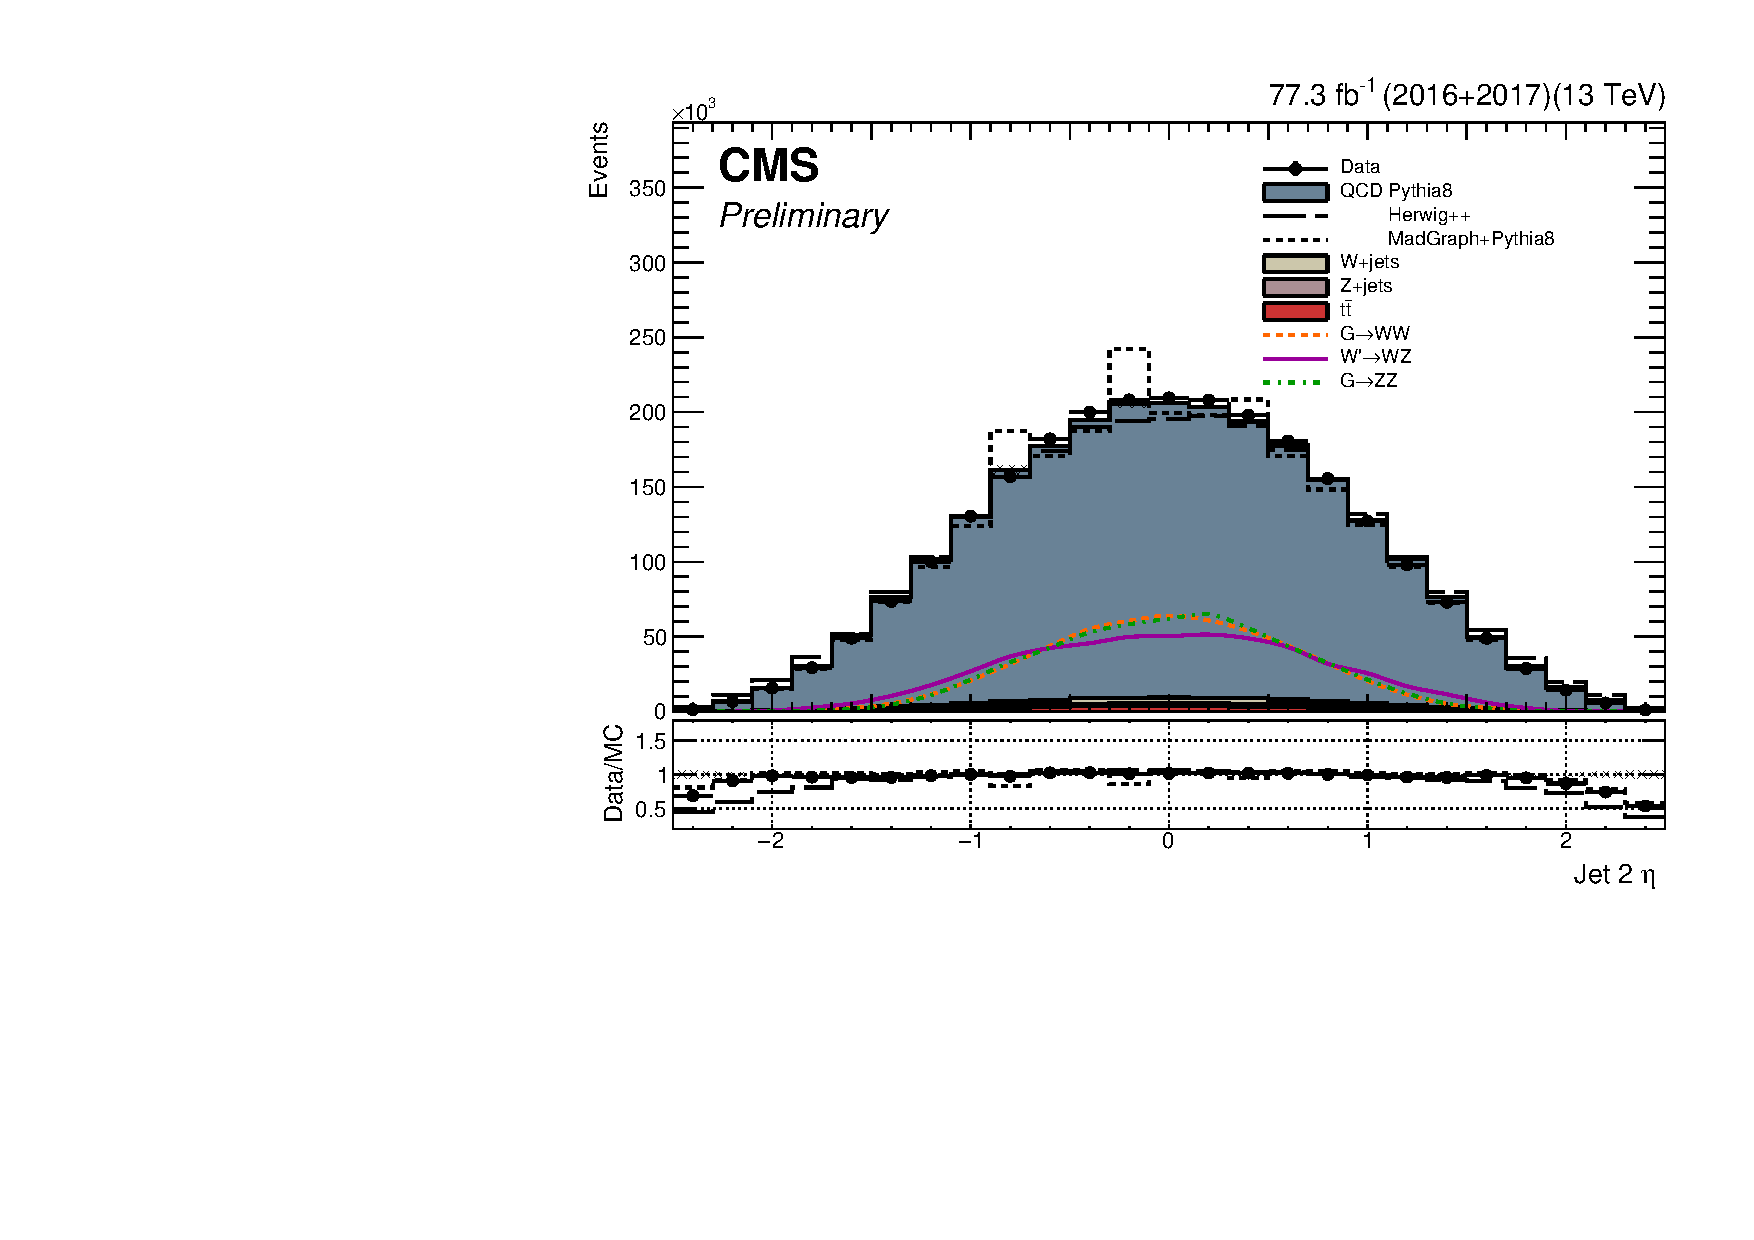
\includegraphics[width=0.450\textwidth]{figures/analysis/search3/AN-17-303/controlPlots/looseSel_Jet_2_eta.pdf}
\caption{Jet \PT{} (top) and $\eta$ (bottom) of the first (left) and second (right) selected jet in the event. The signal is scaled by an arbitrary number.}
\label{fig:kinematics-all}
\end{figure}

\clearpage
\section{Triggering}
\label{sec:searchIII:trigger}
The triggers used for the data collected in 2016 are the same as in Section~\ref{sec:searchI:trigger}, while the thresholds in 2017 have increased in order to push the trigger rate to a level acceptable for the increased luminosity. The triggers used for 2017 data are
\begin{itemize}
  \itemsep0em
\item {HLT\_PFHT1050}
\item {HLT\_AK8PFJet500}
\item {HLT\_AK8PFJet360/380/400/420\_TrimMass30}
\item {HLT\_AK8PFHT750/800/850/900\_TrimMass50}.
\end{itemize}
As in Section~\ref{sec:searchI:trigger}, the trigger names indicate the primary selection criteria, with the terms "PF", "HT", and "AK8" being previously explained. The term "JetXXX" refers to the lower value of the \PT selection criteria of the jet, "HTXXX" refers to the HT requirement, and "TrimMassYY" refers to the trimmed-jet mass selection applied to least one jet. For the results presented here, the analysis threshold is set by the value of \MVV such that the combination of all triggers are greater than $99 \%$ efficient. The trigger turn-on is evaluated in an orthogonal data set in which the presence of a single muon with a \PT above 27 or 50 GeV is required. The trigger efficiency as a function of dijet invariant mass using a combination of all triggers (left), and as a function of the jet soft drop mass for the grooming-based triggers only (right) are shown in Figure~\ref{fig:trigturnon}. The grooming-based triggers in the 2017 data set do not fully reach the trigger plateau as the triggers where unavailable during one data taking period, corresponding to 4.8 \fbinv. 
\begin{figure}[h!]
\centering 
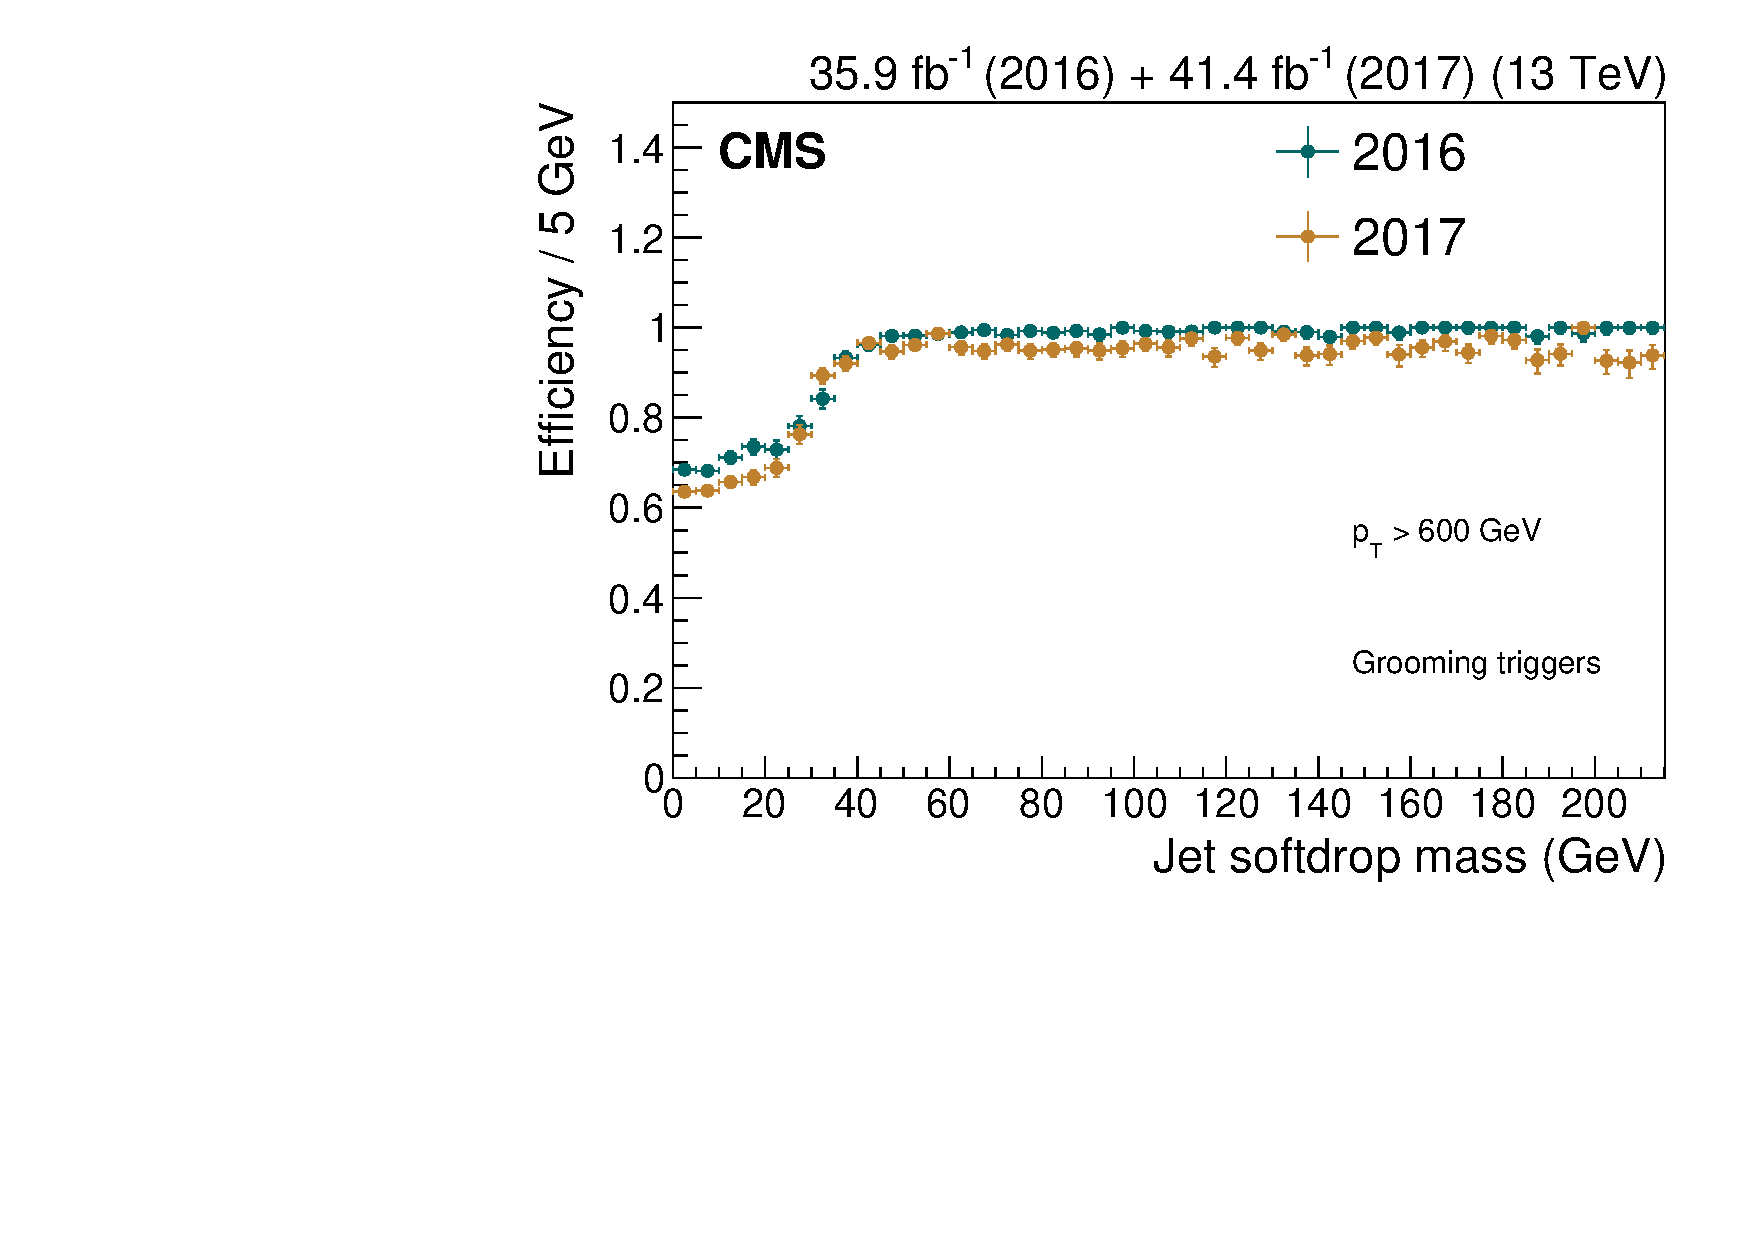
\includegraphics[width=0.45\textwidth]{figures/analysis/search3/B2G-18-002/Combined_mj1_16vs17.pdf}
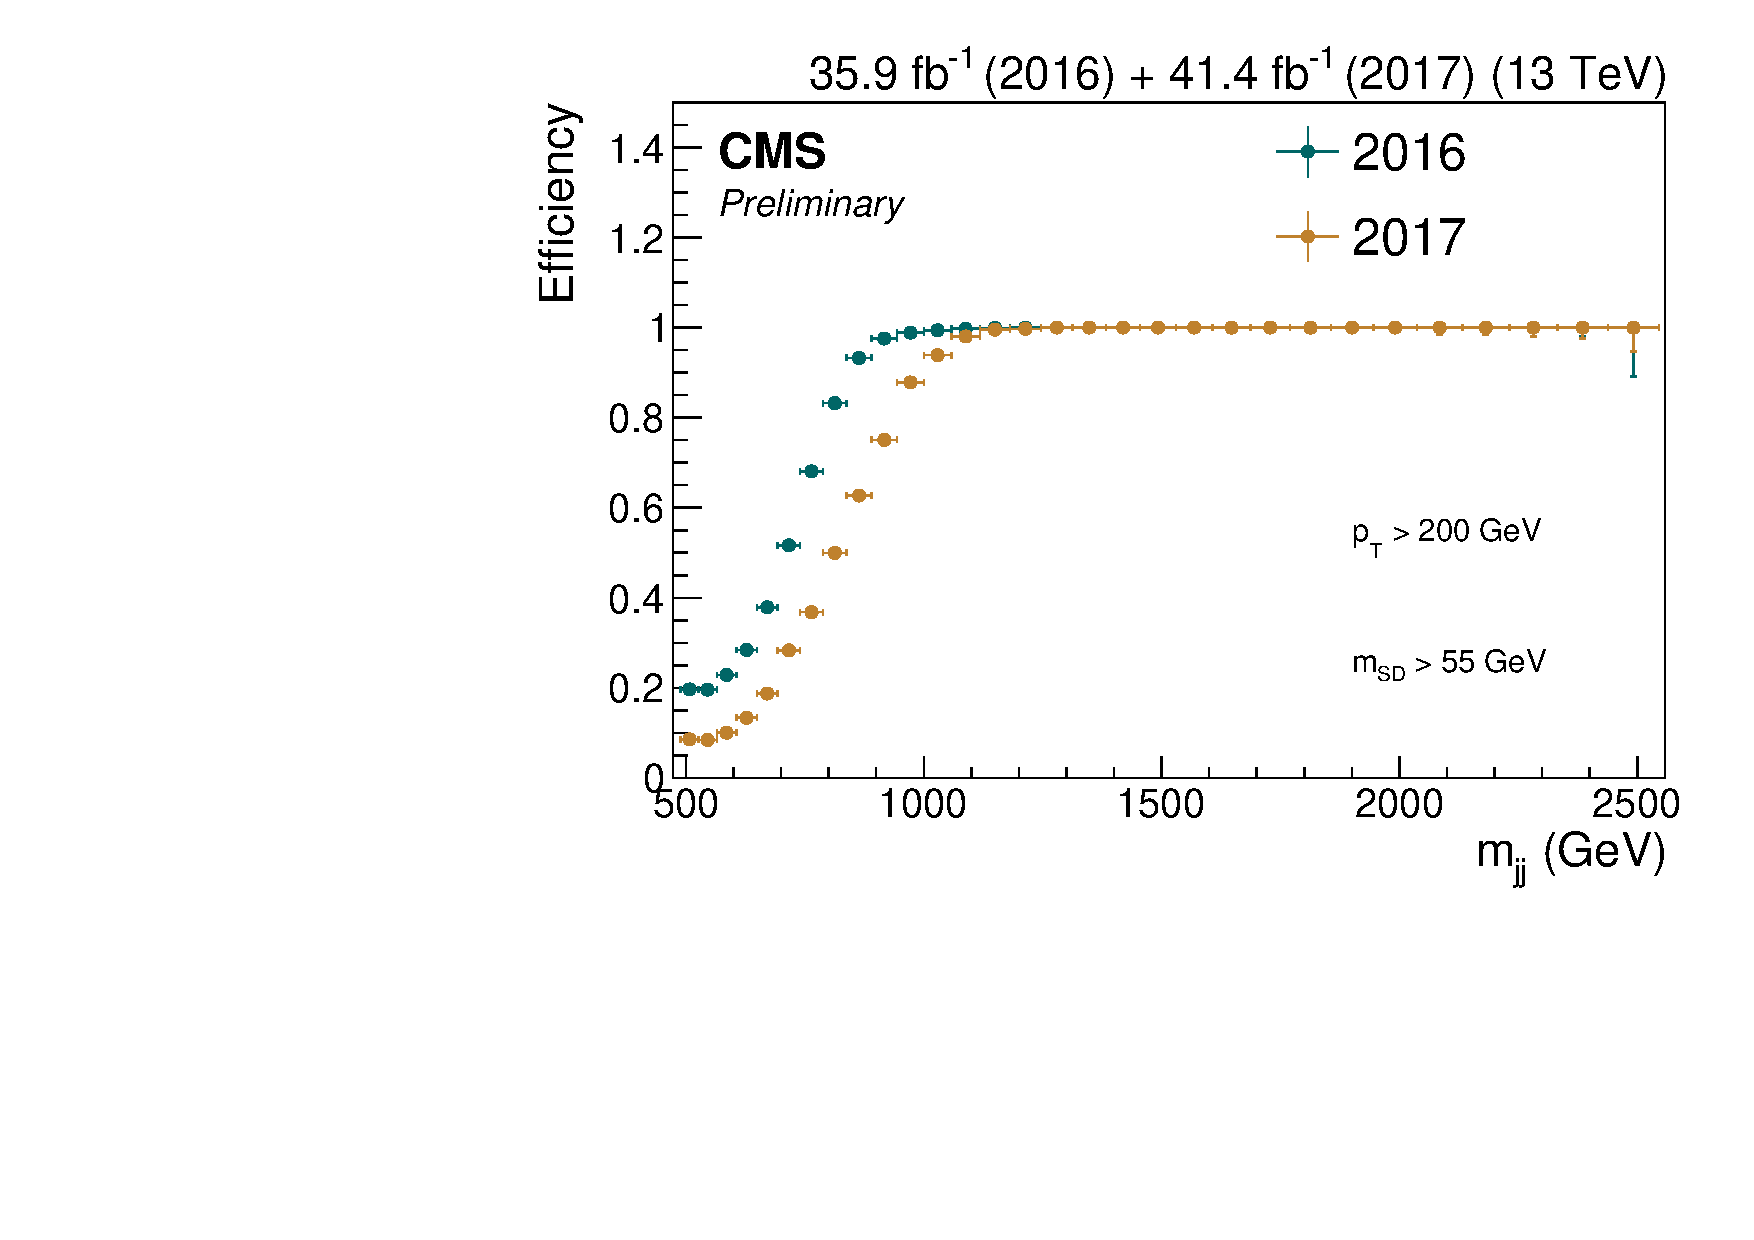
\includegraphics[width=0.45\textwidth]{figures/analysis/search3/B2G-18-002/Combined_mjj_16vs17.pdf}
\caption{Left: trigger efficiency as a function of the dijet invariant mass using a combination of all analysis triggers. Right: trigger efficiency as a function of the jet softdrop mass for triggers requiring an online trimmed mass of at least 30 or 50 \GeV.}
\label{fig:trigturnon}
\end{figure}
The corresponding turn-on excluding the data taken without grooming-based triggers included, is shown in Figure~\ref{fig:trigturnon_noRunB}. Here we see the that the trigger efficiency as a function of jet softdrop mass reaches the trigger plateau at the same point as in 2016.
\begin{figure}[h!]
\centering 
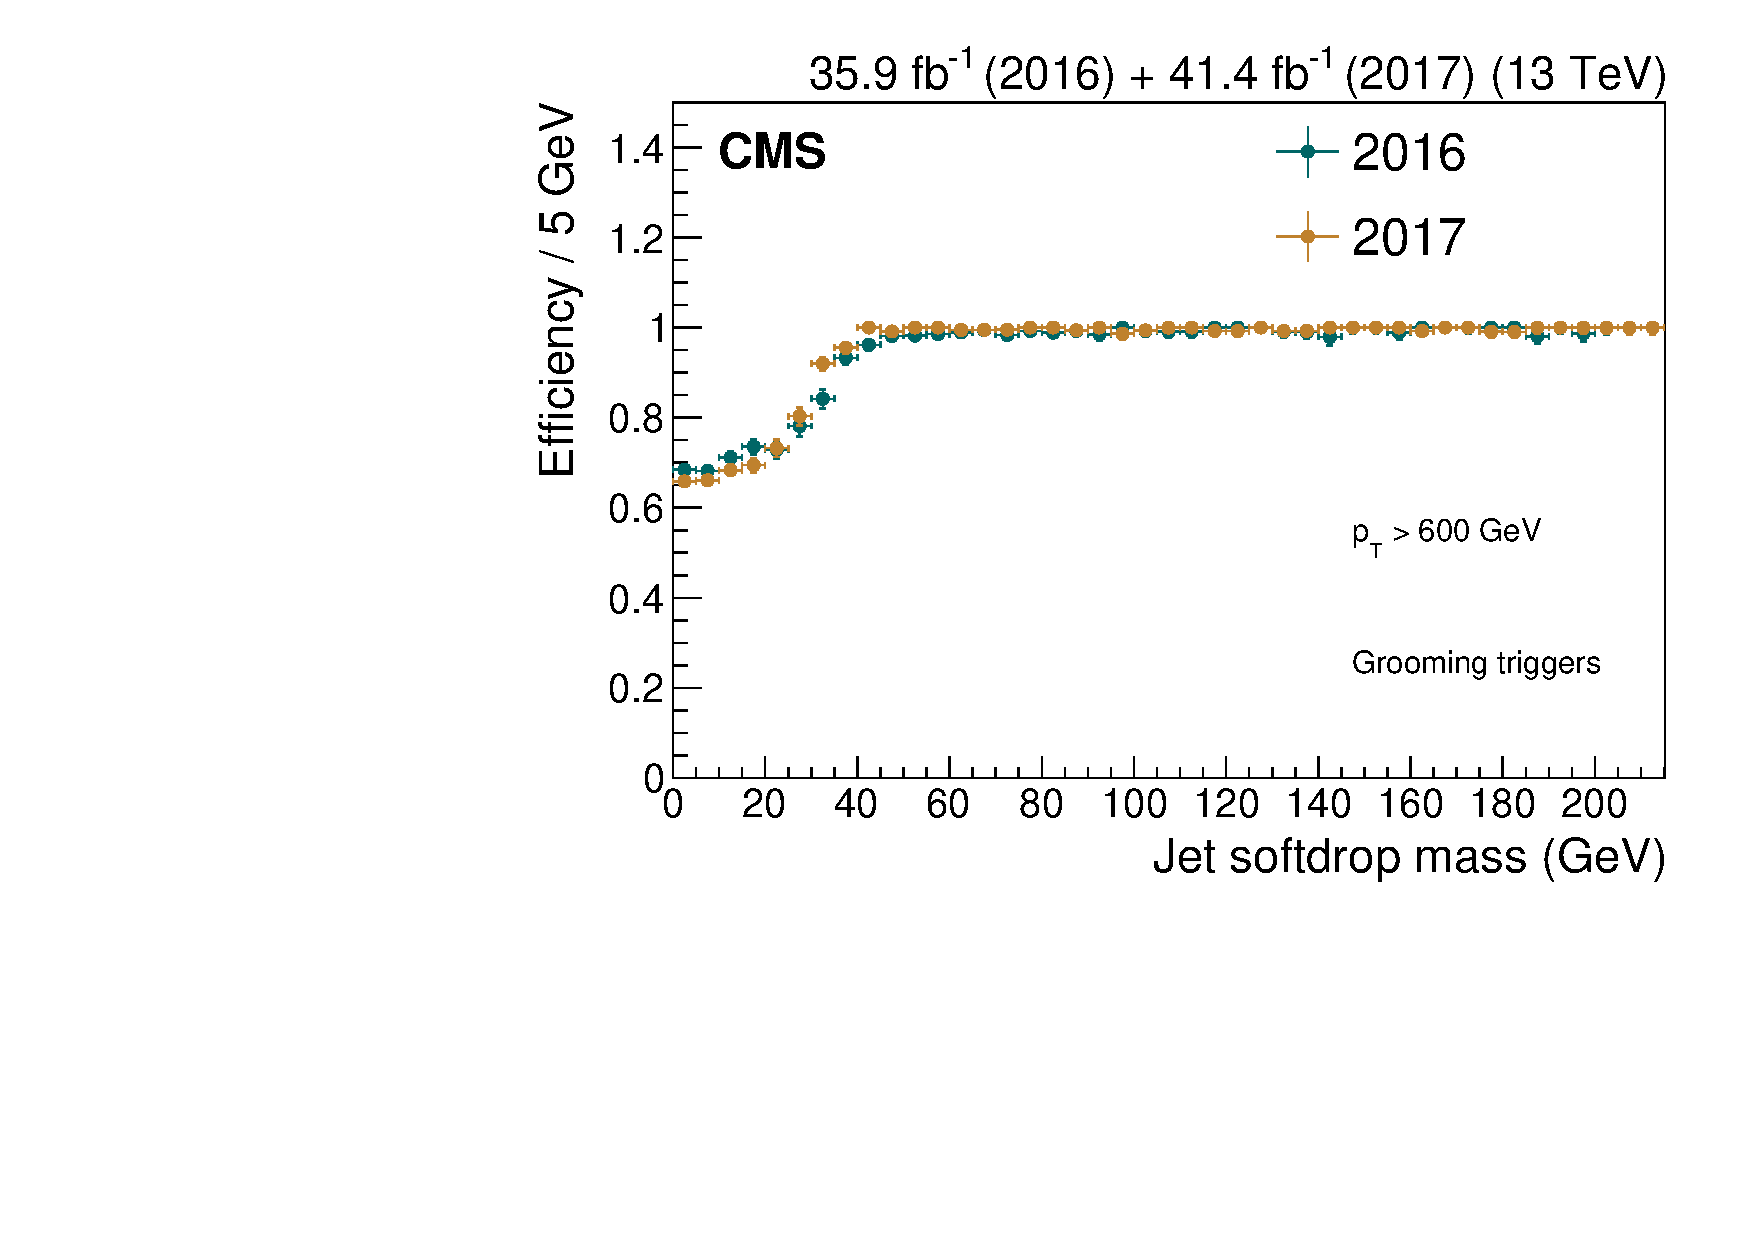
\includegraphics[width=0.45\textwidth]{figures/analysis/search3/B2G-18-002/Combined_noRunB_mj1_16vs17.pdf}
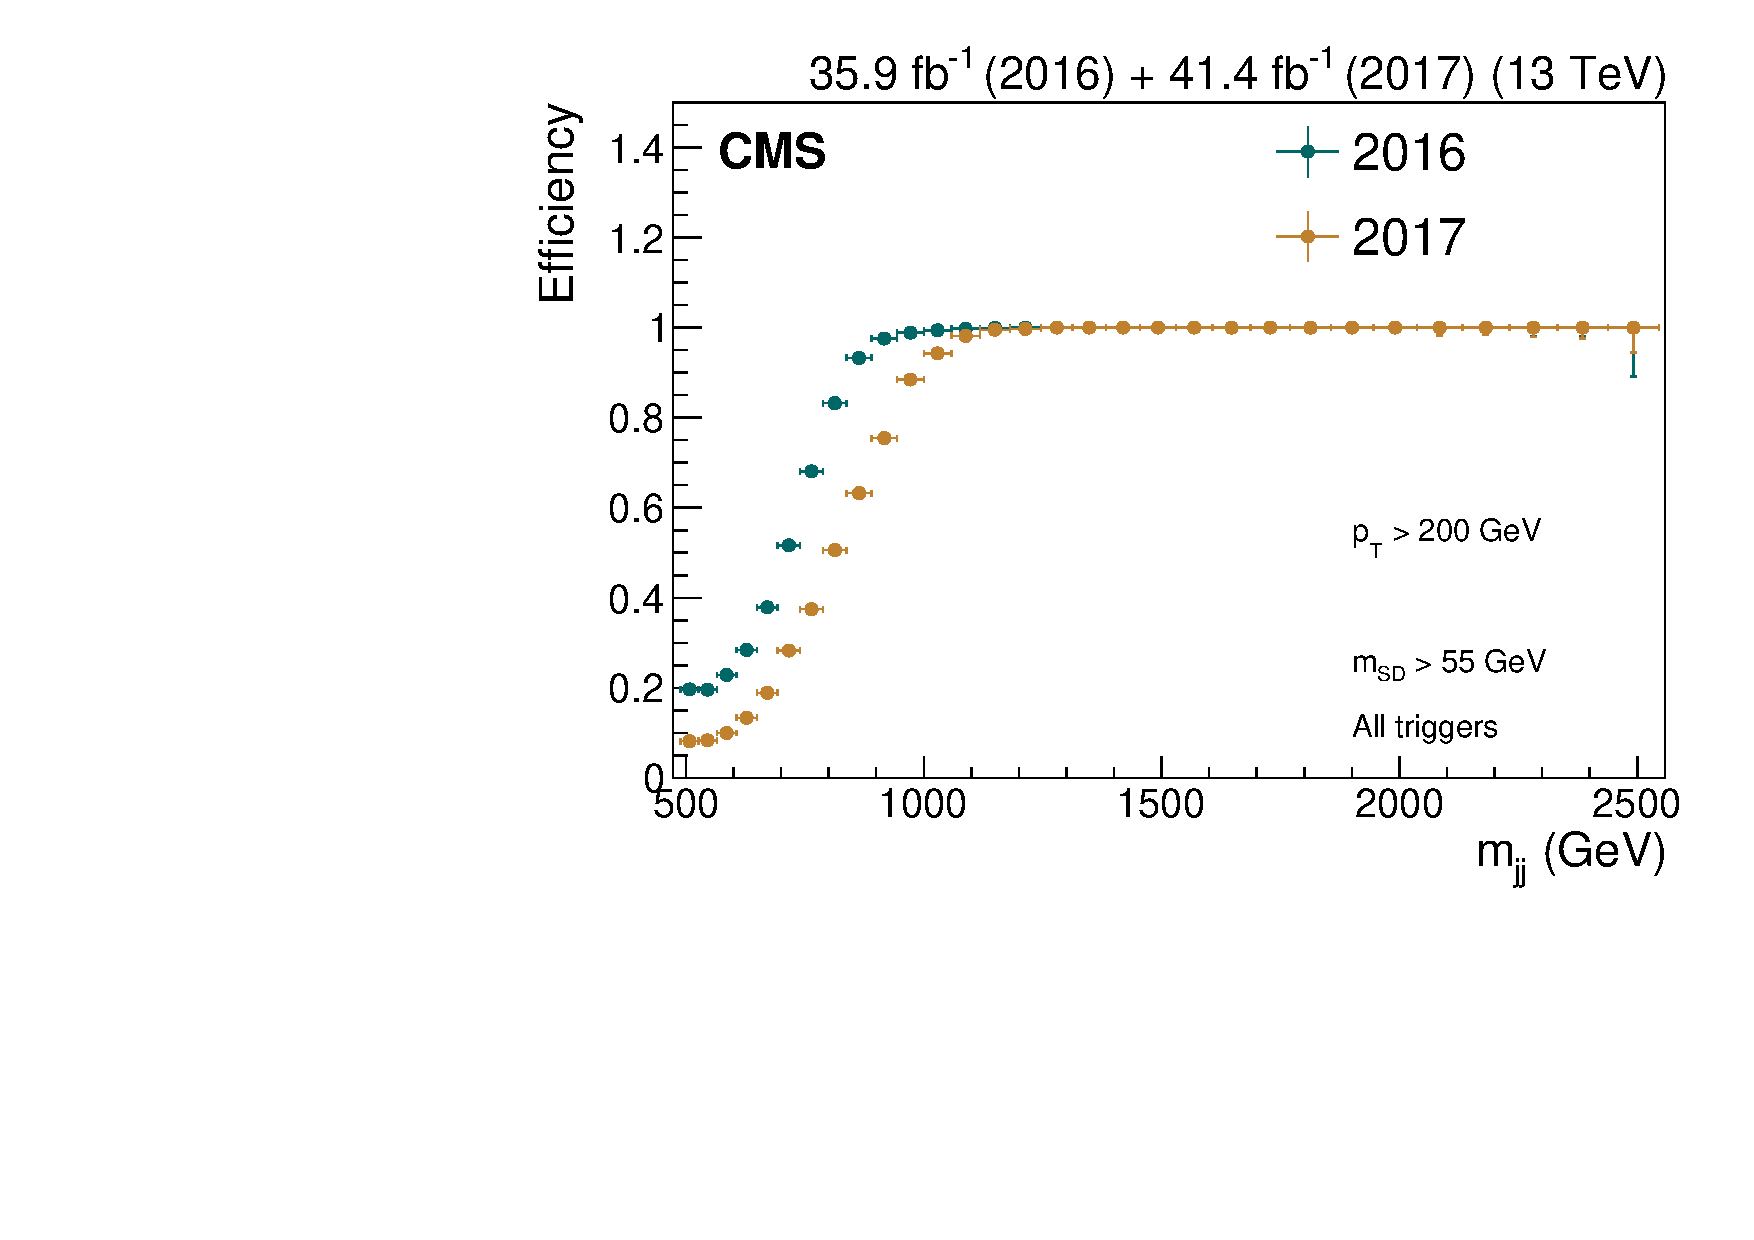
\includegraphics[width=0.45\textwidth]{figures/analysis/search3/B2G-18-002/Combined_noRunB_mjj_16vs17.pdf}
\caption{Left: trigger efficiency as a function of the dijet invariant mass using a combination of all analysis triggers. Right: trigger efficiency as a function of the jet softdrop mass for triggers requiring an online trimmed mass of at least 30 or 50 \GeV. Here after excluding the data taken in 2017 without grooming-based triggers included.}
\label{fig:trigturnon_noRunB}
\end{figure}
The combination of all triggers are $>99\%$ efficient above a dijet invariant mass of 1126 (990) \GeV for the 2017 (2016) dataset. Since the point of full efficiency is largest in the 2017 dataset, this sets the analysis threshold. 

\subsection{Trigger turn-on modeling}
\label{sec:searchIII:triggermodeling}
The threshold in the dijet mass at which resonances can be searched for depends on the value which the trigger can efficiently select events. The threshold used in the previous analyses was required to be high enough so that the dijet mass spectrum could be described with a smoothly falling function. Since the background modeling for this analysis does not depend on a smoothly falling dijet invariant-mass spectrum, as will be described in detail in Section~\ref{sec:searchIII:fit3d}, and in order to compensate for a loss in acceptance due to the increased trigger thresholds, we sought to model the trigger turn-on directly from data. This would allow us to search for diboson resonances with masses below the value at which the trigger is fully efficient. To model the trigger turn-on we derive a three dimensional histogram of the trigger efficiency versus dijet invariant mass ($\MVV$) and the groomed-jet mass of jet 1 and jet 2 ($\MJO$ and $\MJT$), where each bin corresponds to the trigger efficiency for a small range of values of $\MVV$, $\MJO$ and $\MJT$. The procedure is as follows. From the one-dimensional trigger turn-on histograms shown in Figure~\ref{fig:searchIII:trigturnon}, values of M$\MVV$, $\MJO$ and $\MJT$ at which the signal efficiency is above 99\% are determined. For every bin above this threshold, the trigger efficiency is fixed to one, corresponding to a 100\% efficiency. For all bins below this threshold, we fit slices of $\MVV$ in bins of \MJO and \MJT with a sigmoid function, determine the trigger efficiency to be used as a weight for simulated events to pass the trigger, and set the value from this function, and set the bin content of the three dimensional weight histogram accordingly. Since the trigger efficiency falls below 50 percent around a dijet invariant mass of 800 GeV, as seen from the right-hand plot in Figure~\ref{fig:searchIII:trigturnon}, searching for resonances with masses below this point is not feasible due to low acceptance. In addition, the full signal shape needs to be contained within the dijet invariant mass spectrum, requiring the search to consider dijet invariant masses 10\% lower than the actual value of the lowest resonance mass being probed. These two factors dictate that the minimum resonances mass we can search for is 1 TeV, and that the background modeling must begin around 900 GeV in order to fully contain the signal. Starting from a dijet invariant mass of $\MVV=893$ GeV, the "dijet bin" closest to 900 GeV (where the "dijet binning" is as described in Section~\ref{sec:searchI:bkg}), and a jet mass of $\MJ=40$ GeV, a coarsely binned three-dimensional histogram is filled with the fraction of events that pass one of the signal triggers,
\begin{equation*}
w^{Bin}_{ijk}= \frac{\textrm{ PASS}\big(m_{jj}^i,m_{j1}^j,m_{j2}^k\big) }{\textrm{ ALL}\big(m_{jj}^i,m_{j1}^j,m_{j2}^k\big)}.
\end{equation*}
From this three-dimensional coarse histogram, a finer binned histogram is achieved through interpolation. In bins of $\MJO$ and $\MJT$, each slice in $\MVV$ is fitted with a sigmoid function,
\begin{equation*}
s(x)=\frac{1}{1+e^{-p_1(x-p_2)}},
\end{equation*}
and the trigger weight is extracted in dijet invariant mass bins of 10 GeV. This fine binning in dijet invariant mass is sufficient to yield a smooth distribution after trigger reweighting, as will be demonstrated below, and no additional interpolation is done.
% This three-dimensional coarse weight histogram is illustrated in Figure~\ref{fig:3Dtrigger}.
% \begin{figure}[htb]
% \centering
% 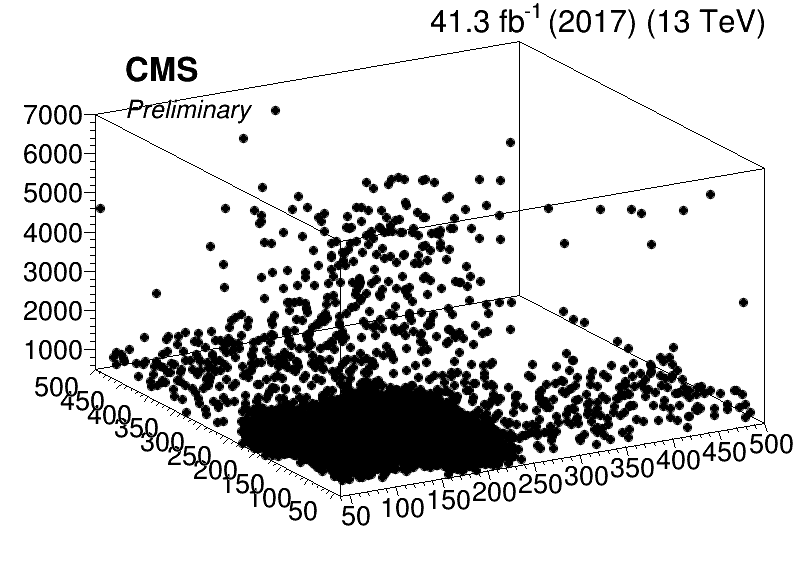
\includegraphics[width=0.45\textwidth]{figures/analysis/search3/AN-17-303/trigger/3D_interpolate.png}
% \caption{Trigger efficiency (coarse) in the three-dimensional $\MVV$-$\MJO$-$\MJT$ plane. }
% \label{fig:3Dtrigger}
% \end{figure}
% An example of two such fits and their corresponding trigger weight in projections of $\MVV$ is shown in Figure~\ref{fig:triggerWeights}.
% \begin{figure}[htb]
% \centering
% 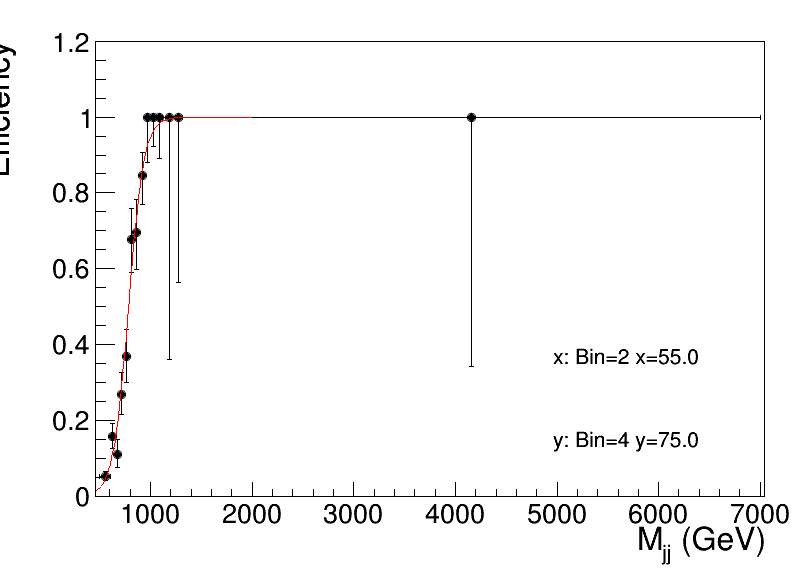
\includegraphics[height=3cm]{figures/analysis/search3/AN-17-303/trigger/x2_y4_fitstatus0.png}
% 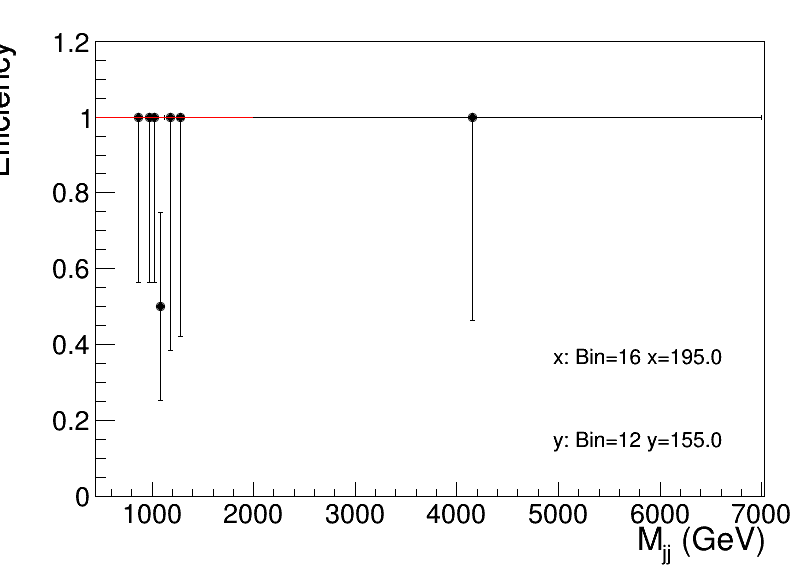
\includegraphics[height=3cm]{figures/analysis/search3/AN-17-303/trigger/x16_y12_fitstatus0.png}\\
% 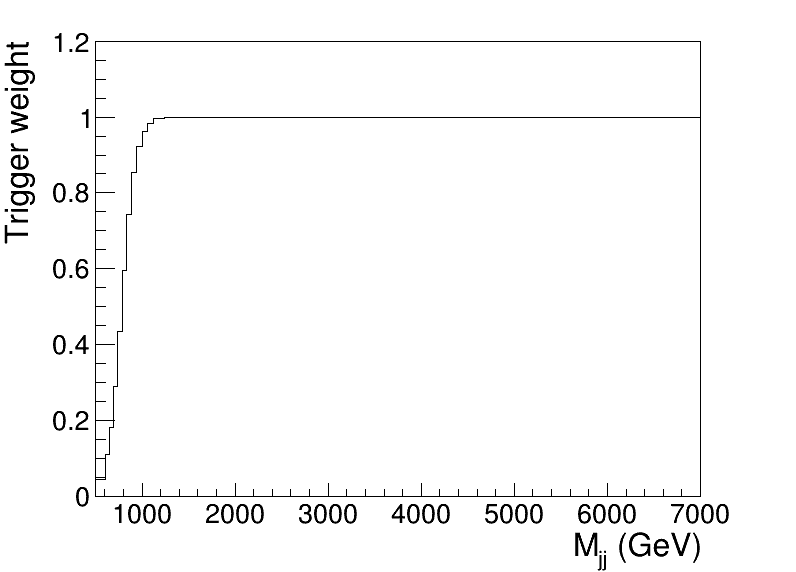
\includegraphics[height=3cm]{figures/analysis/search3/AN-17-303/trigger/x2_y4_weight.png}
% 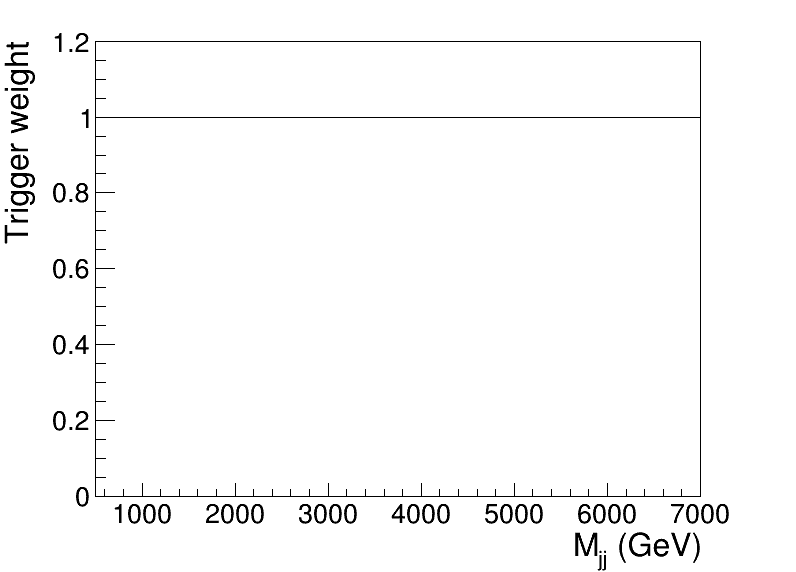
\includegraphics[height=3cm]{figures/analysis/search3/AN-17-303/trigger/x16_y12_weight.png}
% \caption{Fits to the trigger efficiency in slices of $\MVV$ for (top left) a central ($\MJO=55 \GeV$, $\MJT=75 \GeV$) and (top right) an extreme ($\MJO=195 \GeV$, $\MJT=155 \GeV$) bin (top)
% and the corresponding trigger weights derived from the fit (bottom).}
% \label{fig:triggerWeights}
% \end{figure}
Figure~\ref{fig:triggerProj} shows the total projections on the $\MVV$, $\MJO$ and $\MJT$ axes for the full trigger weight histogram.
\begin{figure}[h!]
\centering
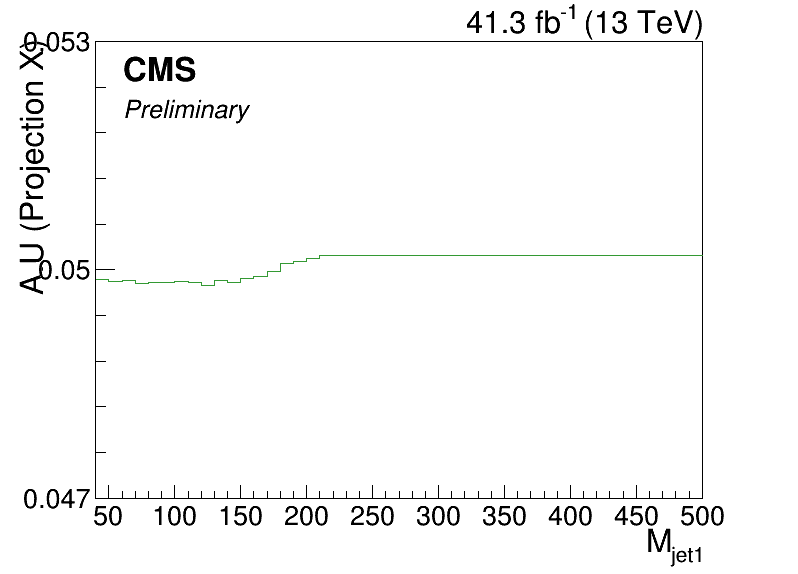
\includegraphics[width=0.3\textwidth]{figures/analysis/search3/AN-17-303/trigger/3D_x.png}
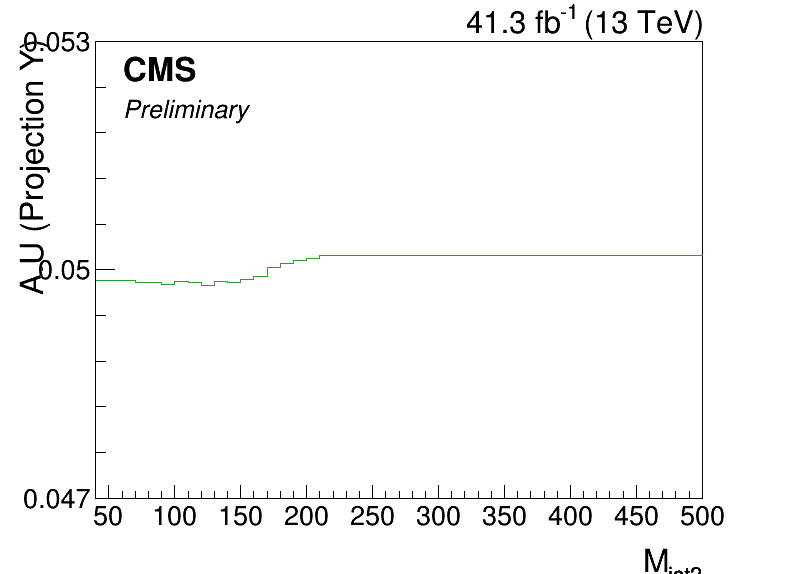
\includegraphics[width=0.3\textwidth]{figures/analysis/search3/AN-17-303/trigger/3D_y.png}
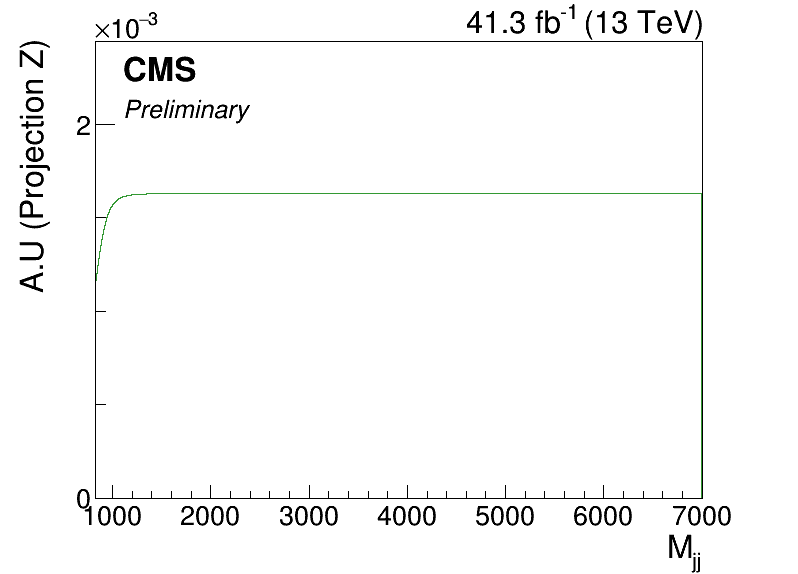
\includegraphics[width=0.3\textwidth]{figures/analysis/search3/AN-17-303/trigger/3D_z.png}
% 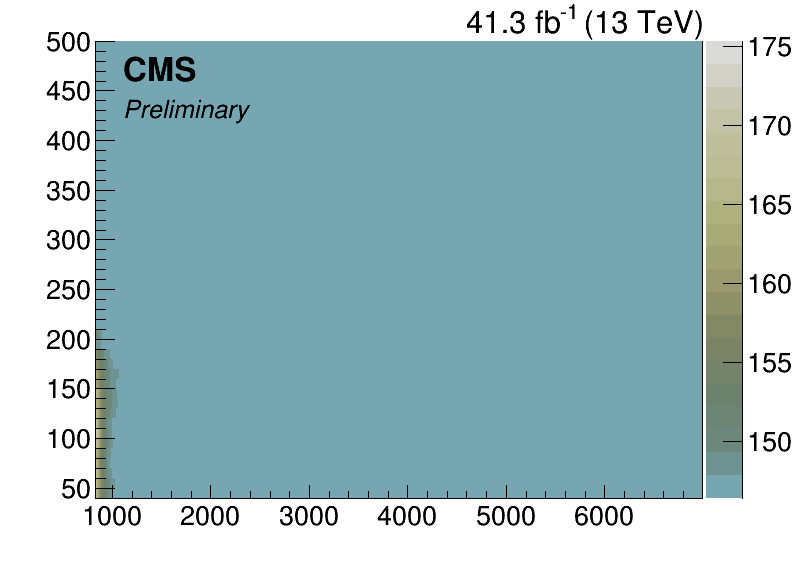
\includegraphics[width=0.3\textwidth]{figures/analysis/search3/AN-17-303/trigger/3D_yz.png}
% 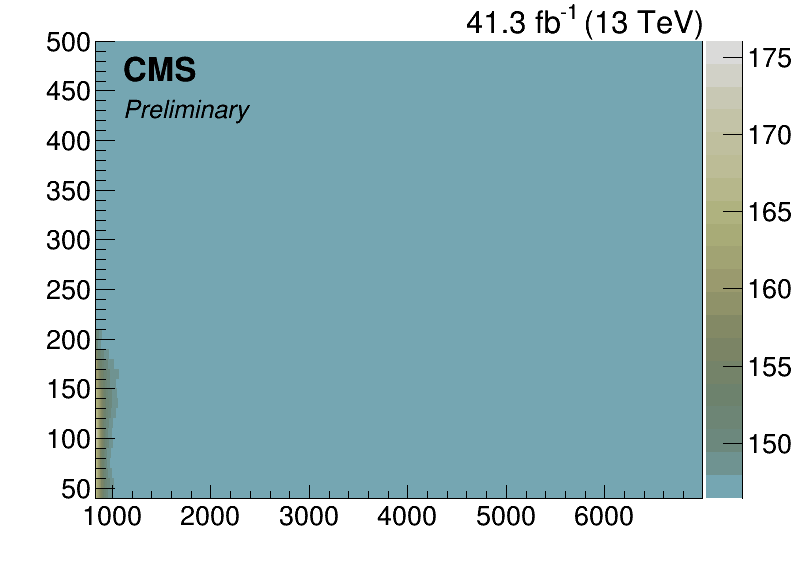
\includegraphics[width=0.3\textwidth]{figures/analysis/search3/AN-17-303/trigger/3D_xz.png}
% 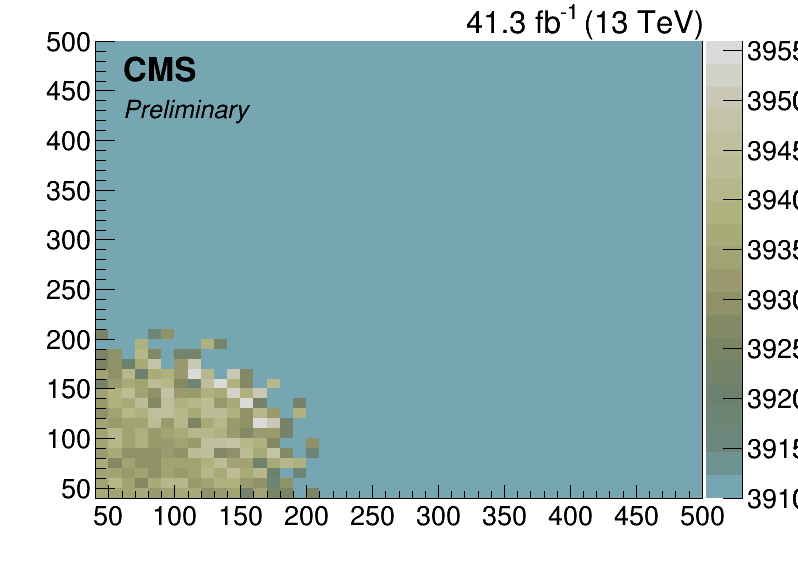
\includegraphics[width=0.3\textwidth]{figures/analysis/search3/AN-17-303/trigger/3D_yx.png}
\caption{One-dimensional projections of the trigger weight histogram for $\MJO$, $\MJT$ and $\MVV$, respectively.}
\label{fig:triggerProj}
\end{figure}
The $\MJ$ and $\MVV$ spectra for the signal sample with the lowest resonance mass, and for the QCD background before and after trigger weights have been applied, are shown in Figure~\ref{fig:triggerMCspectra} and are compared to data. A greater than $95\%$ the signal efficiency is retained after the trigger weights have been applied, and the reweighted QCD simulation agrees well with data.
\begin{figure}[h!]
\centering
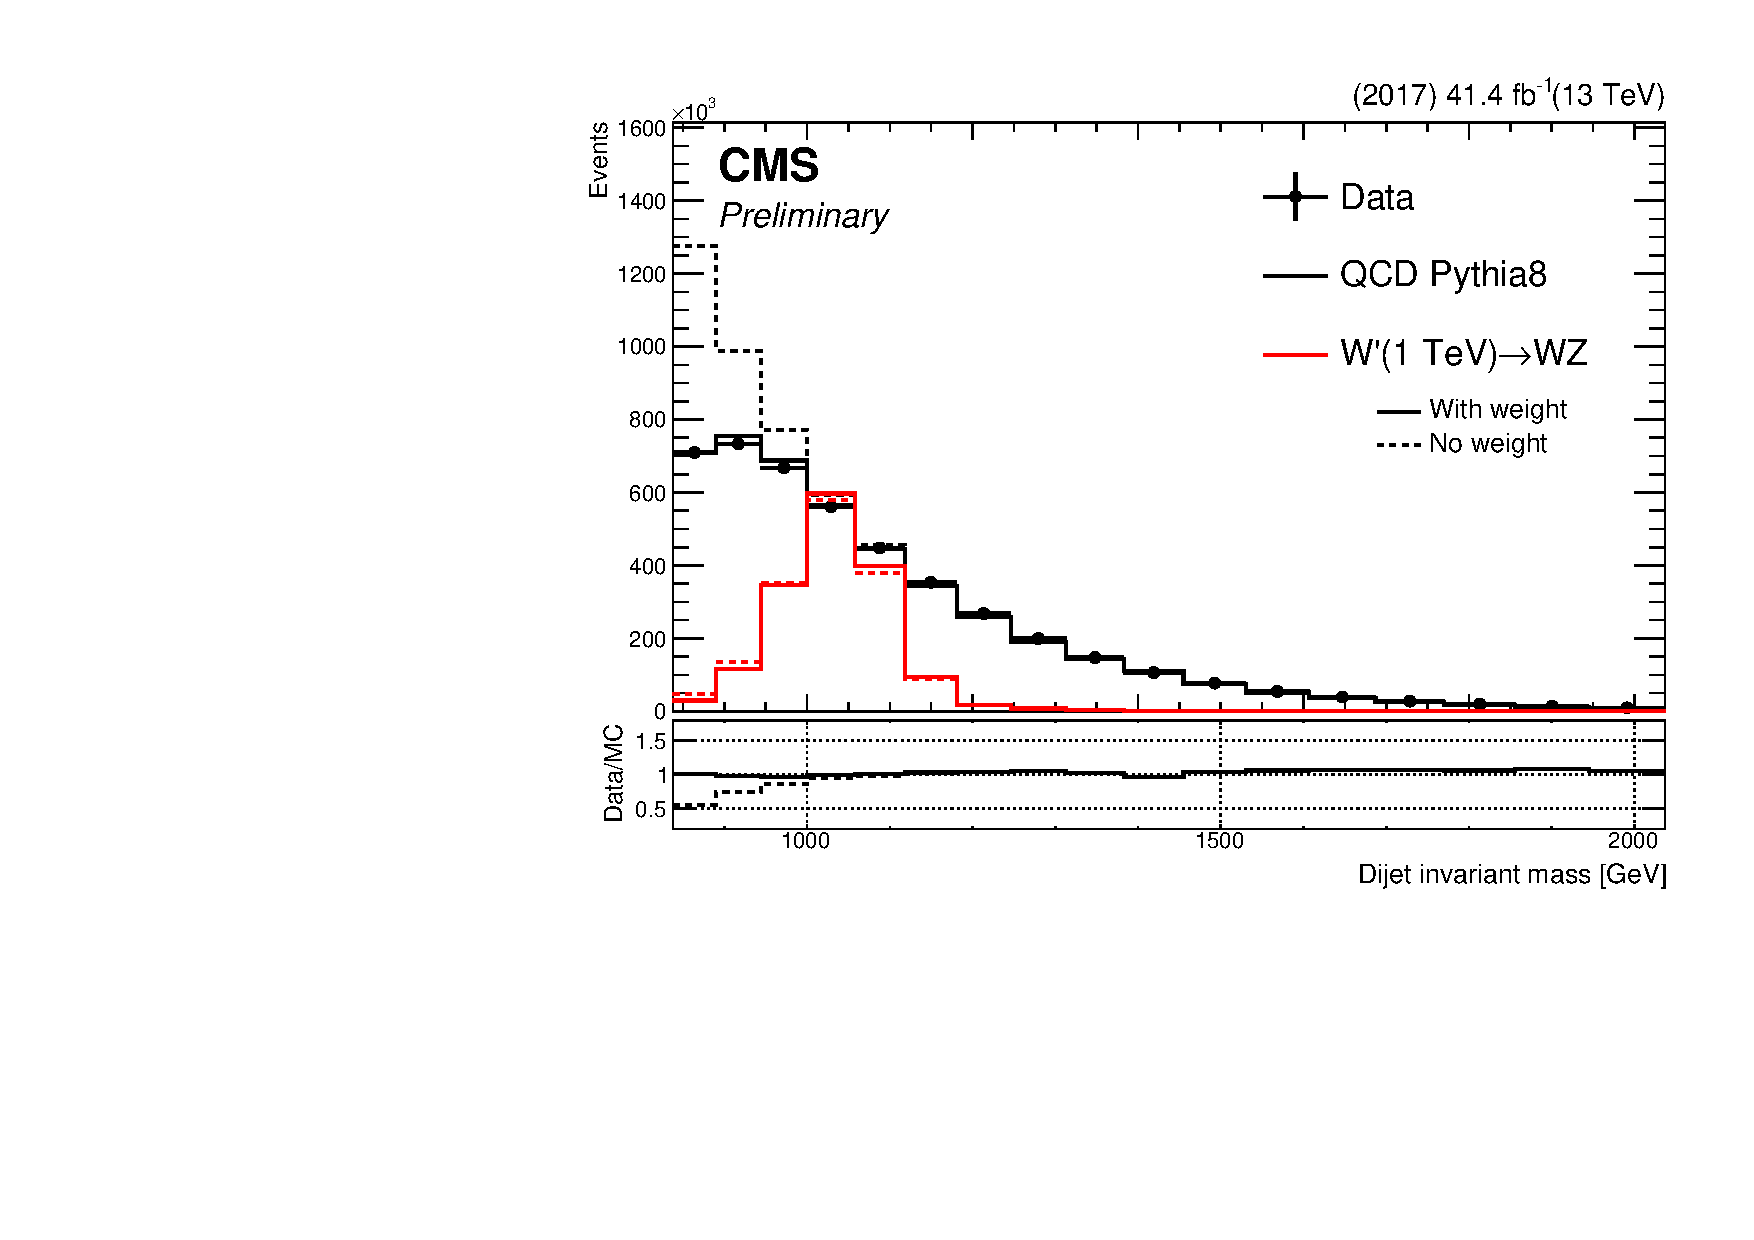
\includegraphics[width=0.49\textwidth]{figures/analysis/search3/B2G-18-002/trigWeightCompare_looseSel_Dijet_invariant_mass.pdf}
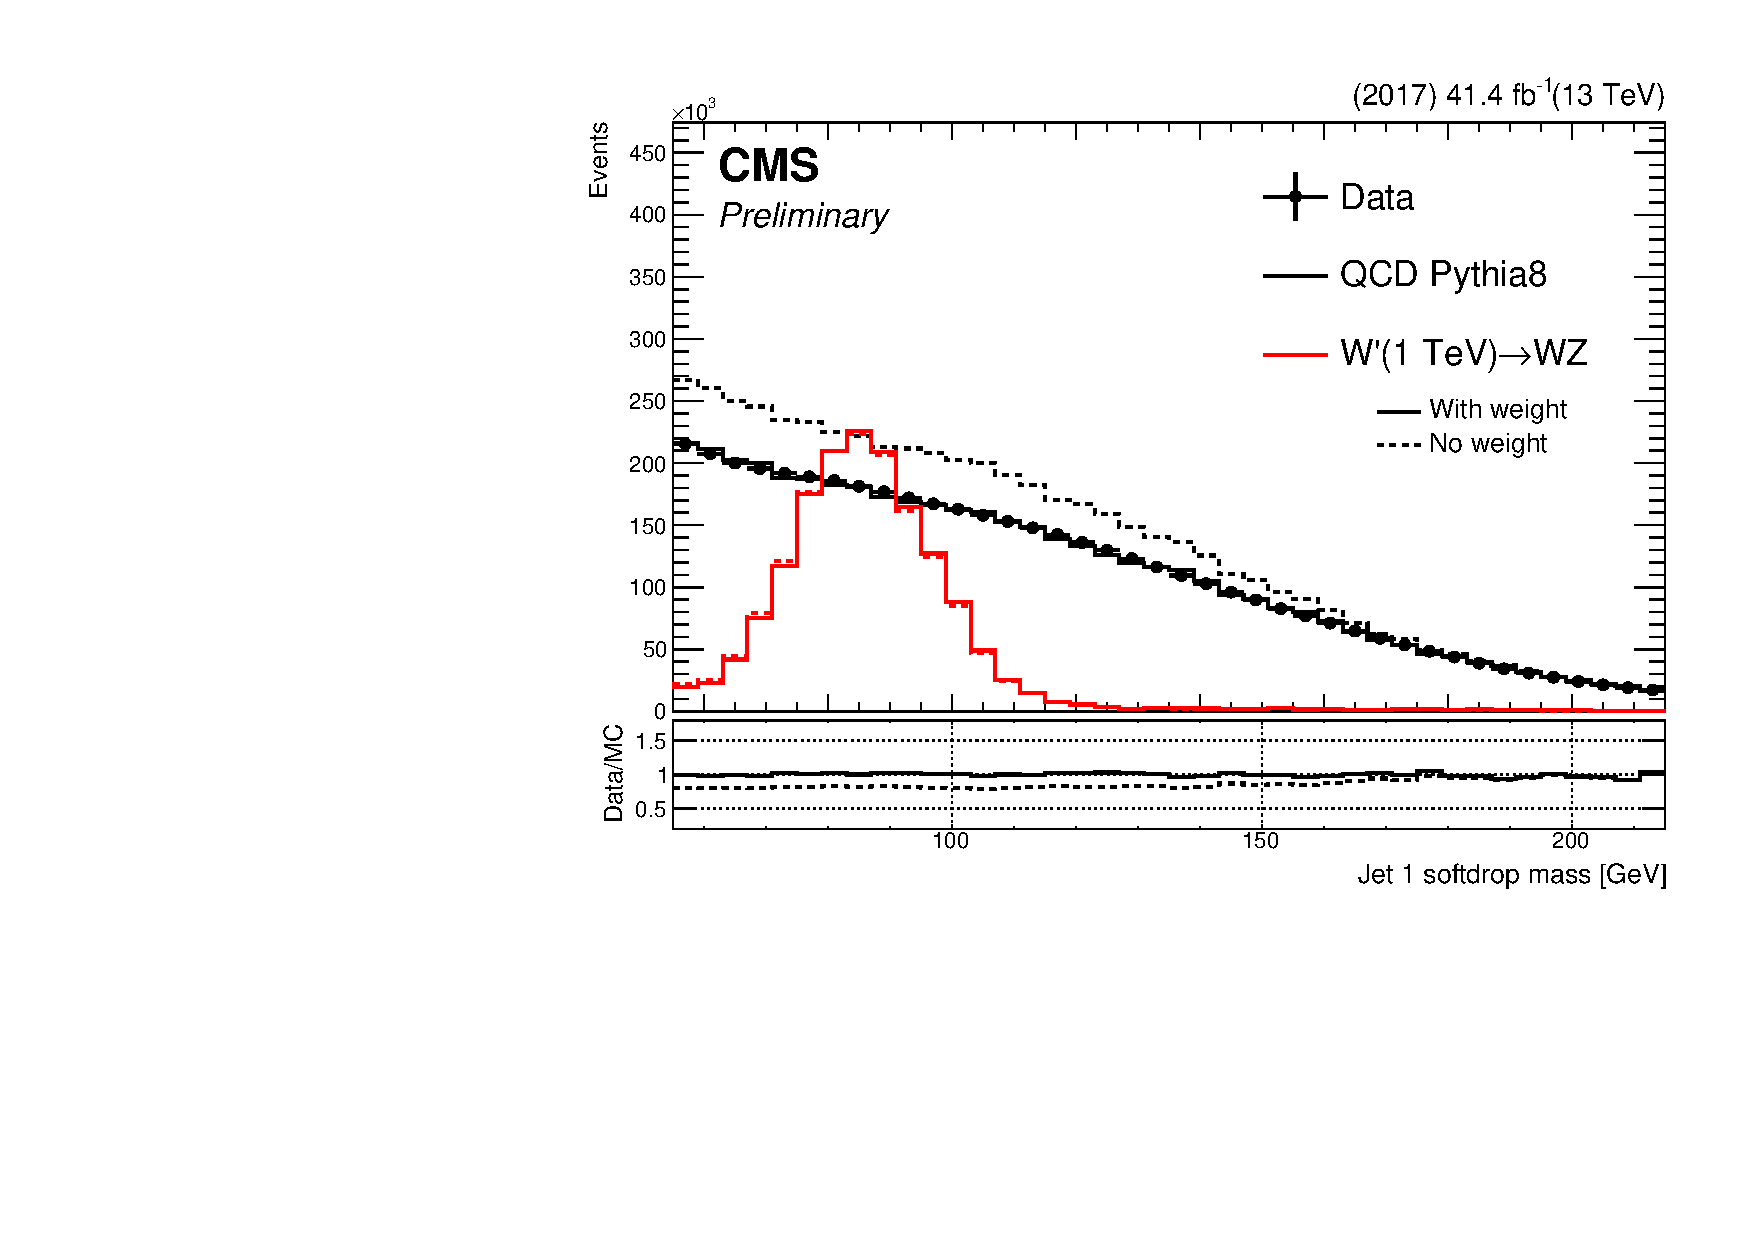
\includegraphics[width=0.49\textwidth]{figures/analysis/search3/B2G-18-002/trigWeightCompare_looseSel_Jet_1_softdrop_mass.pdf}
\caption{The $\MVV$ (left) and $\MJ$ (right) spectra for signal and background before and after trigger weights have been applied.}
\label{fig:triggerMCspectra}
\end{figure}
The modeling of the trigger turn-on was then implemented in the background fit method in the 3D analysis and we found that the method could model the turn-on well. However, when studying the bias on the extracted signal rate for a possible signal in this turn-on region, we found this to be large due to the difficulties involved with fitting a signal peak on top of a background that is peaking. Since the intention of the analysis presented here was to introduce the 3D fit method and allow it to become available as soon as possible, we therefore abandoned the modeling of the trigger turn-on for this paper. However, we still wish to pursue this strategy in the future.
\clearpage

\section{A mass- and \PT-decorrelated tagger}
\label{sec:searchIII:ddt}
In order to identify W-jet and Z-jet candidates we utilize the softdrop algorithm and calculate the n-subjettiness ratio \nsubj for AK8 jets that are clustered with PUPPI constituents. As before, the softdrop jet mass is used to improve the mass resolution of the jet, while n-subjettiness serves as a discriminant by yielding a probability of how compatible the jet is with having N axes. For this search we require the softdrop jet mass to be between $\unit{55} < m_{sd} < \unit{215}{\GeV}$, removing as much as possible of the low-mass QCD background and going high enough to encompass all searches for resonances decaying to W, Z, H or tops (the SM particles known to produce jets with substructure in the final state). Since the analysis is done in bins of jet mass and dijet invariant mass, the background must be modeled for a very wide range of mass and transverse momenta. It is therefore desirable that the QCD background spectrum is minimally sculpted as a function of \PT and mass, such that the background shapes in all regions are similar to one another and remains smoothly falling in all three analysis dimensions and in all bins of $\MVV$, $\MJO$ and $\MJT$. In order to ensure minimal sculpting, we therefore decorrelate the \nsubj variable from the jet softdrop mass and the jet \PT following what was done in Ref.~\cite{Dolen:2016kst}, and briefly discussed in Section~\ref{sec:searchII:vtagperf}. This decorrelation is performed by flattening the $\tau_{21}$ profile dependence on $\rho'$, where $\rho'$ is defined by
\begin{equation}
\rho' = log(m^2/p_T/\mu) \textrm{, where $\mu$ = 1 GeV}.
\end{equation}
Figure~\ref{fig:rho} shows the profile distribution of $\tau_{21}$ as a function of $\rho'$ for QCD jets after applying the preselections listed above together with a softdrop mass selection of $\unit{55} < m_{sd} < \unit{215}{\GeV}$.
% before (left) and after (right) applying a softdrop mass selection of $\unit{55}{\GeV} < m_{sd} < \unit{215}{\GeV}$ (right).
\begin{figure}[h!]
\centering
\begin{tabular}{cc}
% 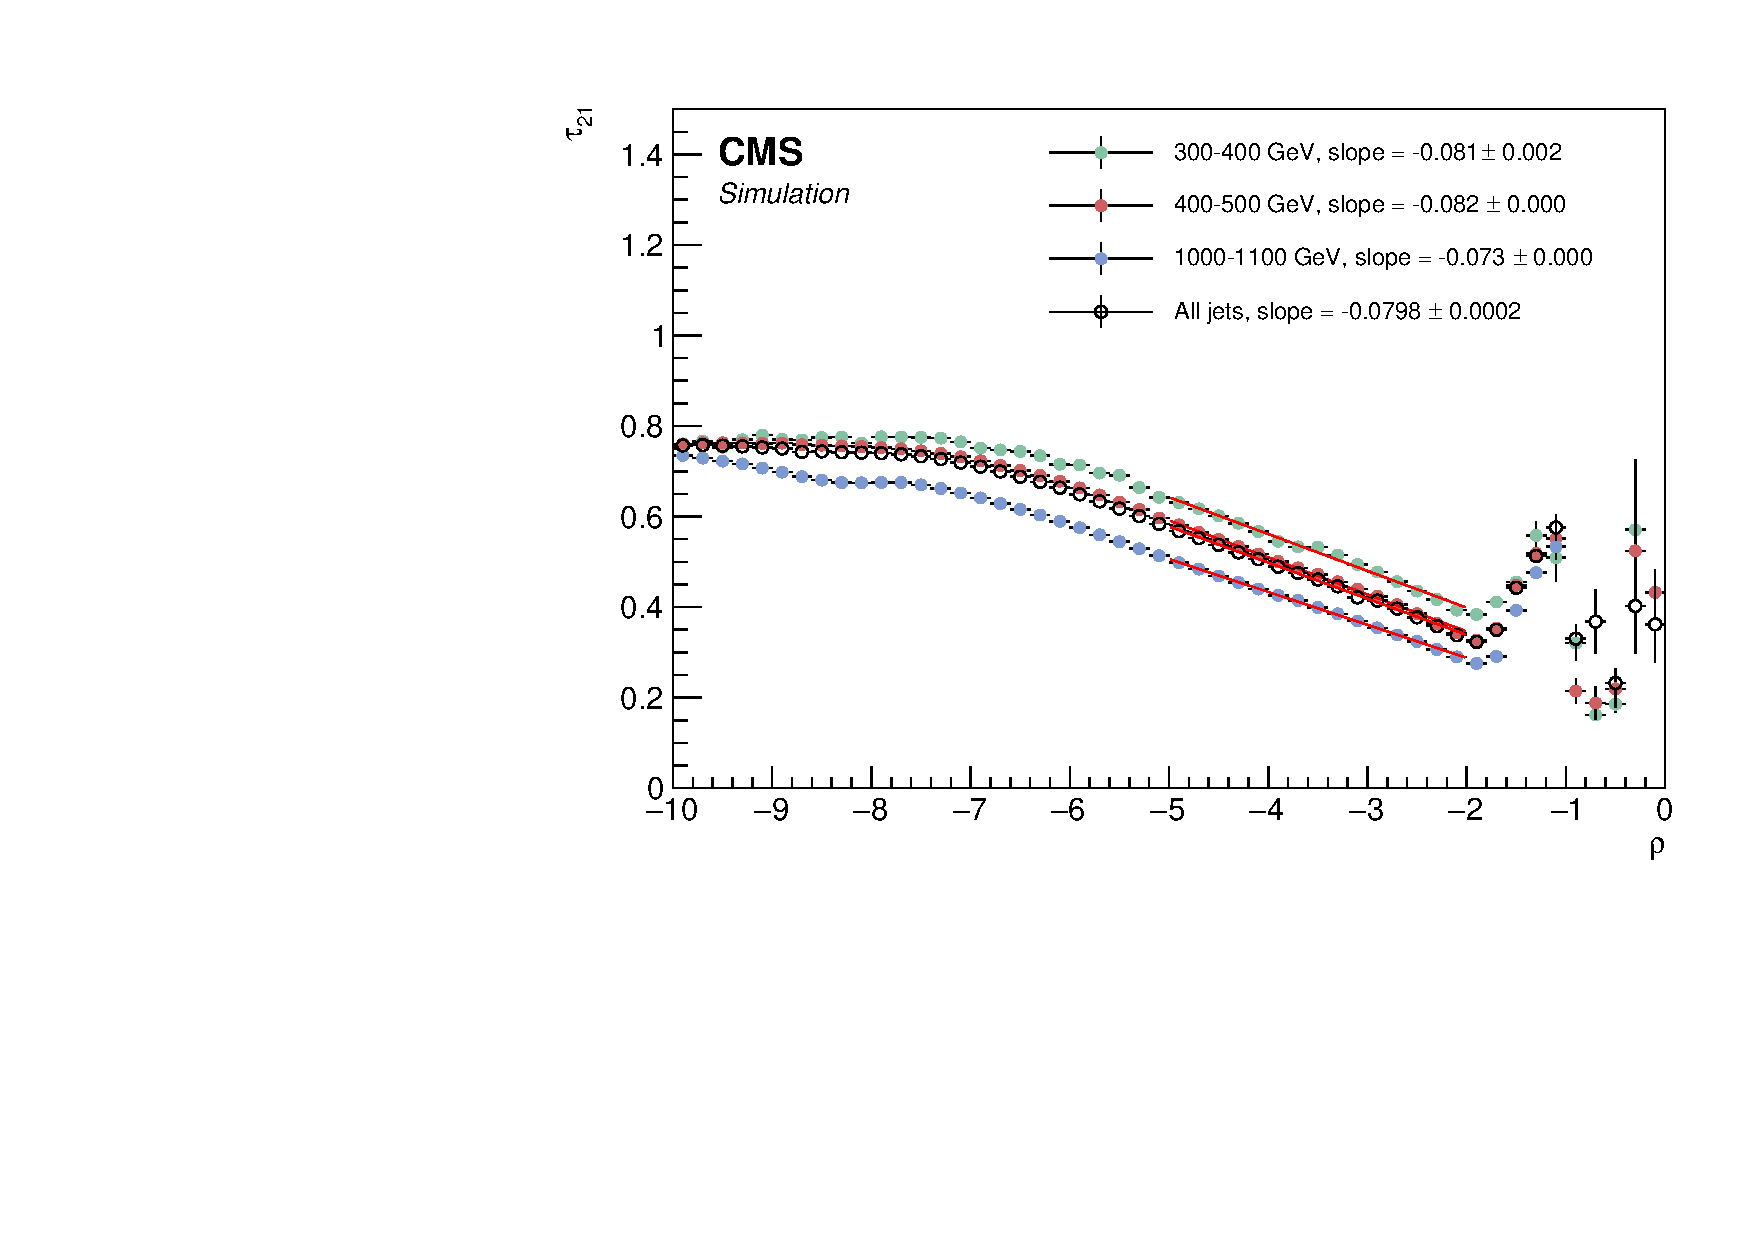
\includegraphics[width=0.45\textwidth]{figures/analysis/search3/AN-17-303/vtag/rho_pythia.pdf}
% 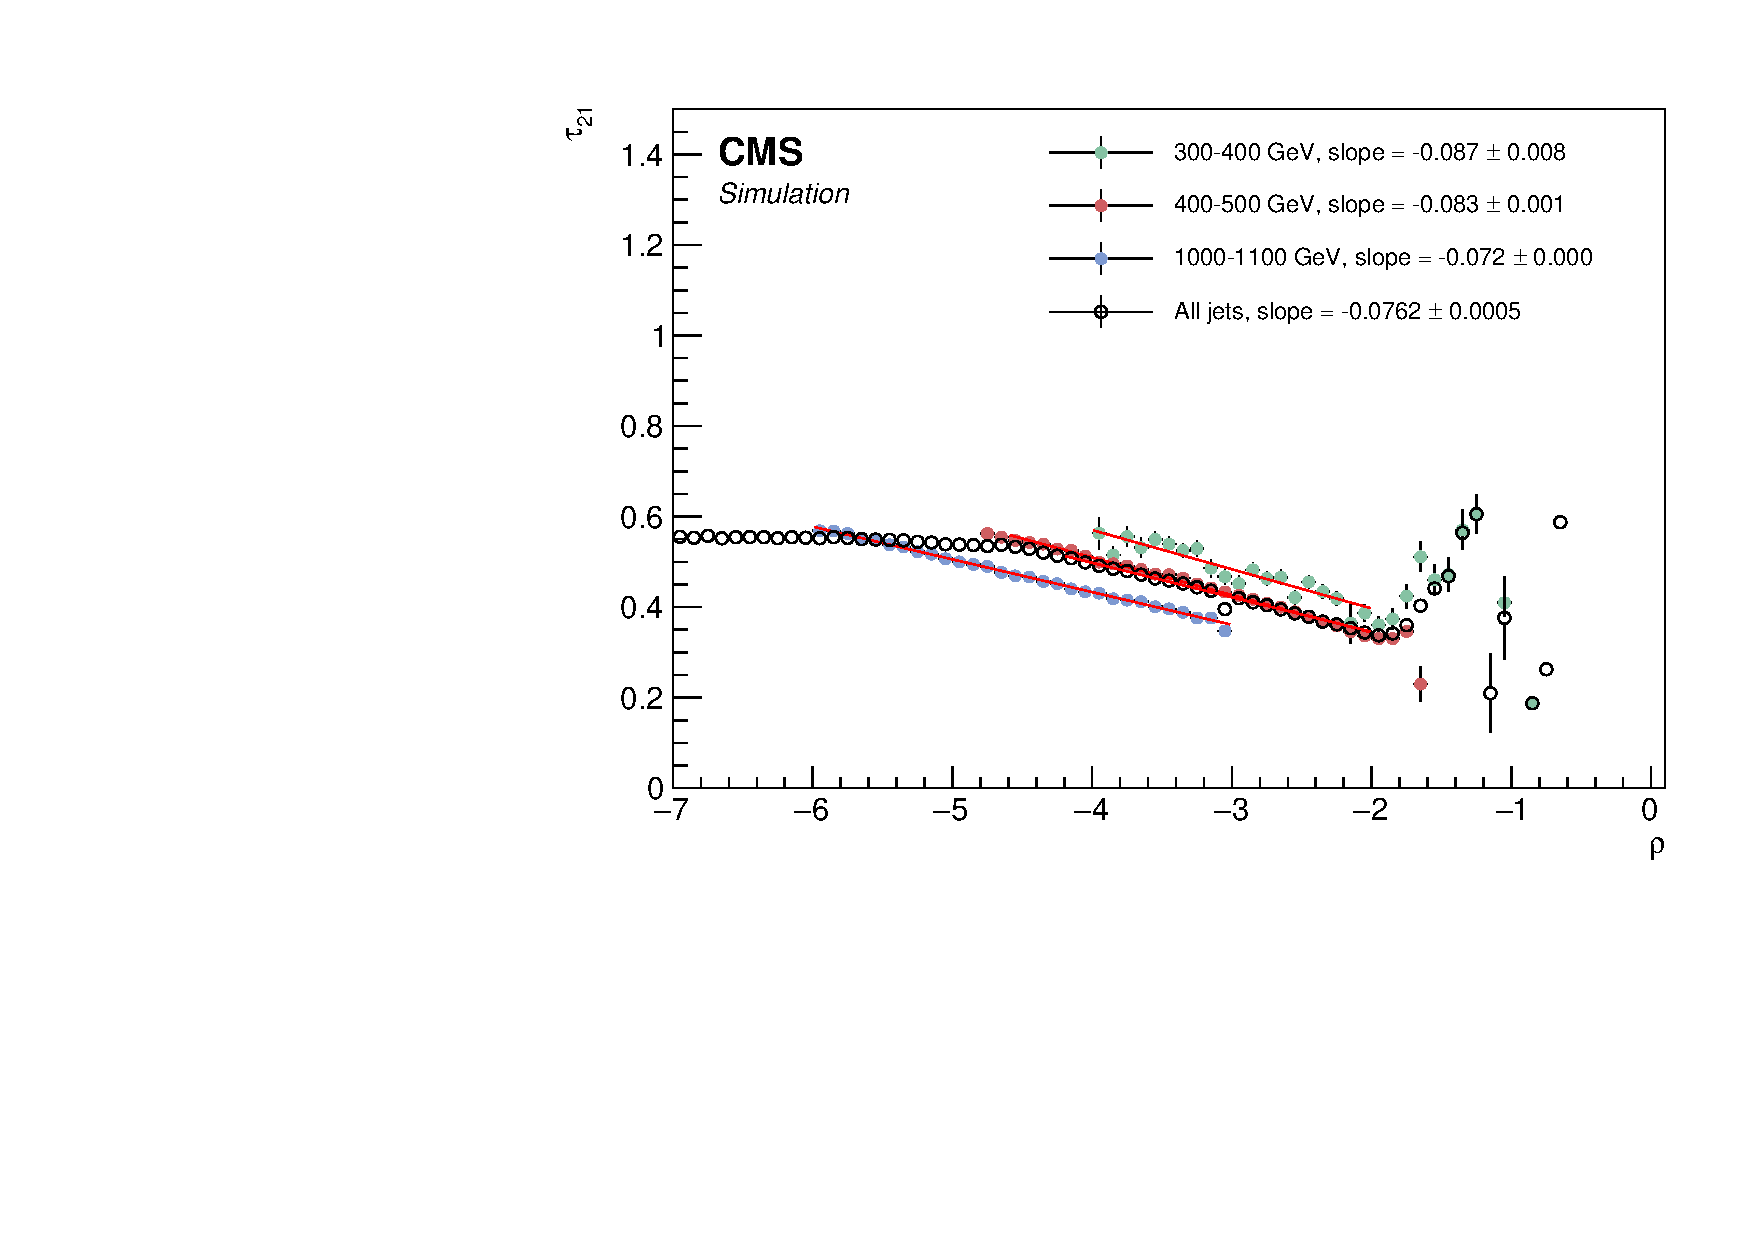
\includegraphics[width=0.45\textwidth]{figures/analysis/search3/AN-17-303/vtag/rho_pythia_FullSel.pdf}\\
% 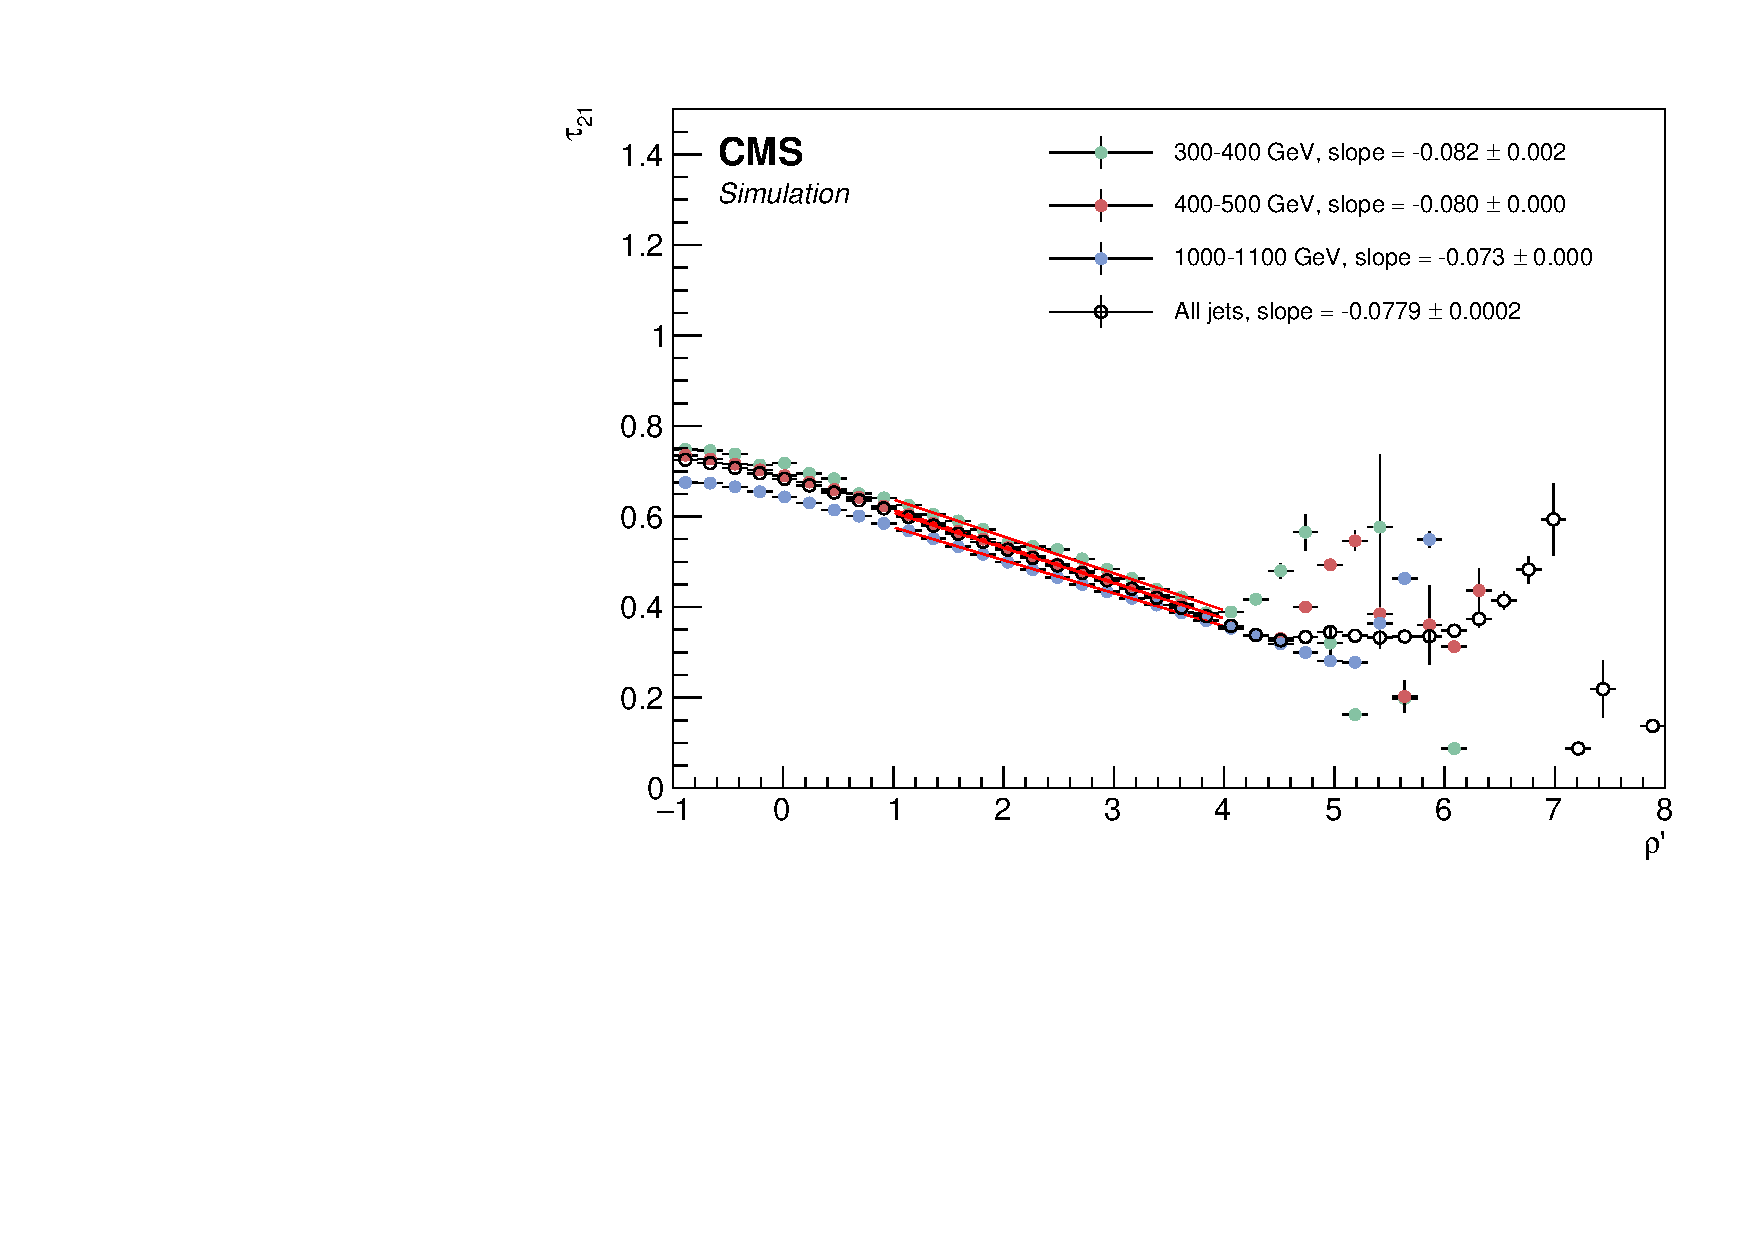
\includegraphics[width=0.45\textwidth]{figures/analysis/search3/AN-17-303/vtag/rho_pythia_rhoPrime.pdf}
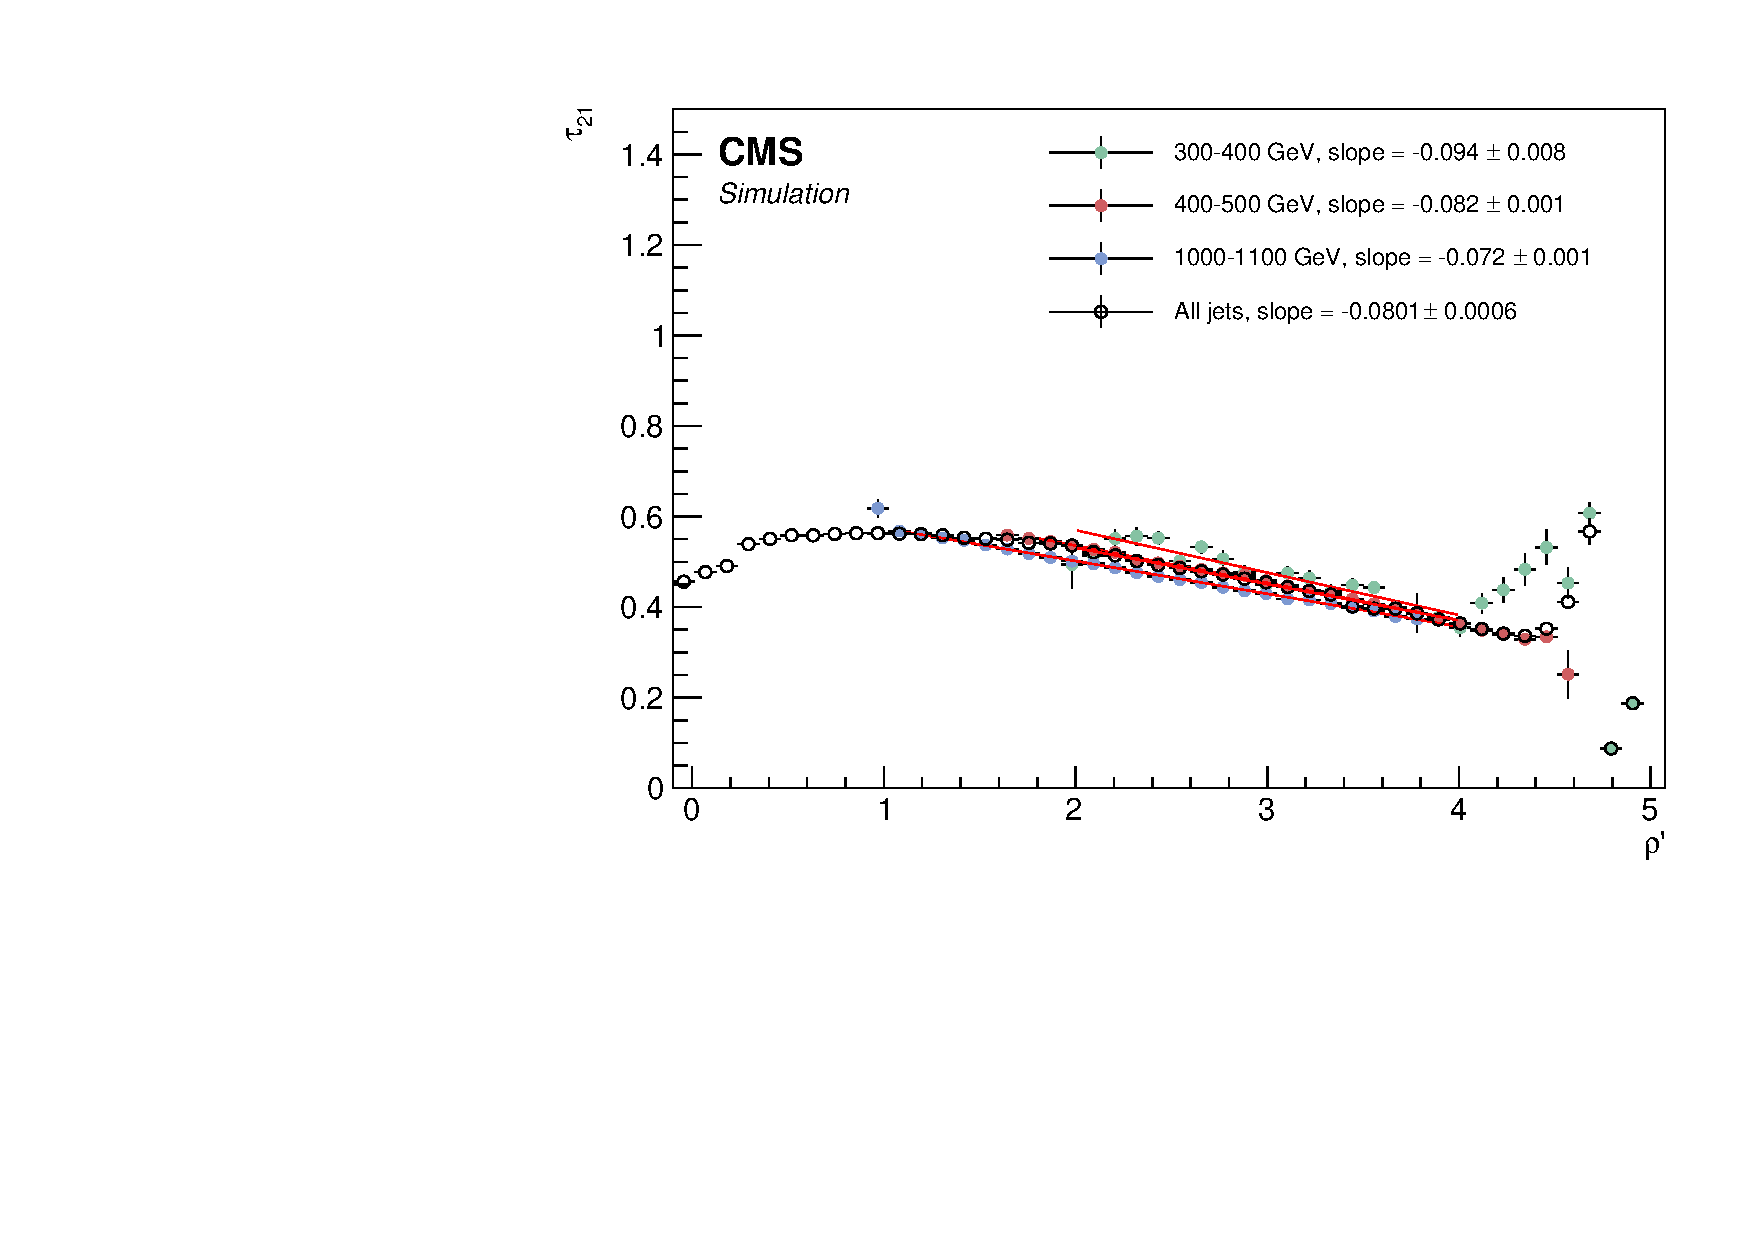
\includegraphics[width=0.45\textwidth]{figures/analysis/search3/AN-17-303/vtag/rho_pythia_FullSel_rhoPrime.pdf}\\
\end{tabular}
\caption{Profile distributions of $\tau_{21}$ as a function of $\rho' = log(m^2/p_T/\mu)$ after applying a softdrop mass selection of $\unit{55} < m_{sd} < \unit{215}{\GeV}$.}
\label{fig:rho}
\end{figure}
A linear transformation is then defined as
\begin{equation}
\label{eq:ddt}
\tau_{21}^{DDT}=\tau_{21}-M\times\rho',
\end{equation}
where the slope M is fitted from the linear part of the $\tau_{21}$ profile versus $\rho'$ for the inclusive \PT spectrum, shown in Figure~\ref{fig:rho}. The resulting slope is $\ensuremath{M} = -0.080$.
%, slightly steeper than the value that was used of $\ensuremath{M} = -0.063$~\cite{JME-16-003}.
The profile of the retuned $\tau_{21}^{DDT}$ versus $\rho'$ is shown in Figure~\ref{fig:rhoClosure}, exhibiting the desired flattened spectra for QCD jets versus $\rho'$.
\begin{figure}[h!]
\centering
\begin{tabular}{cc}
% 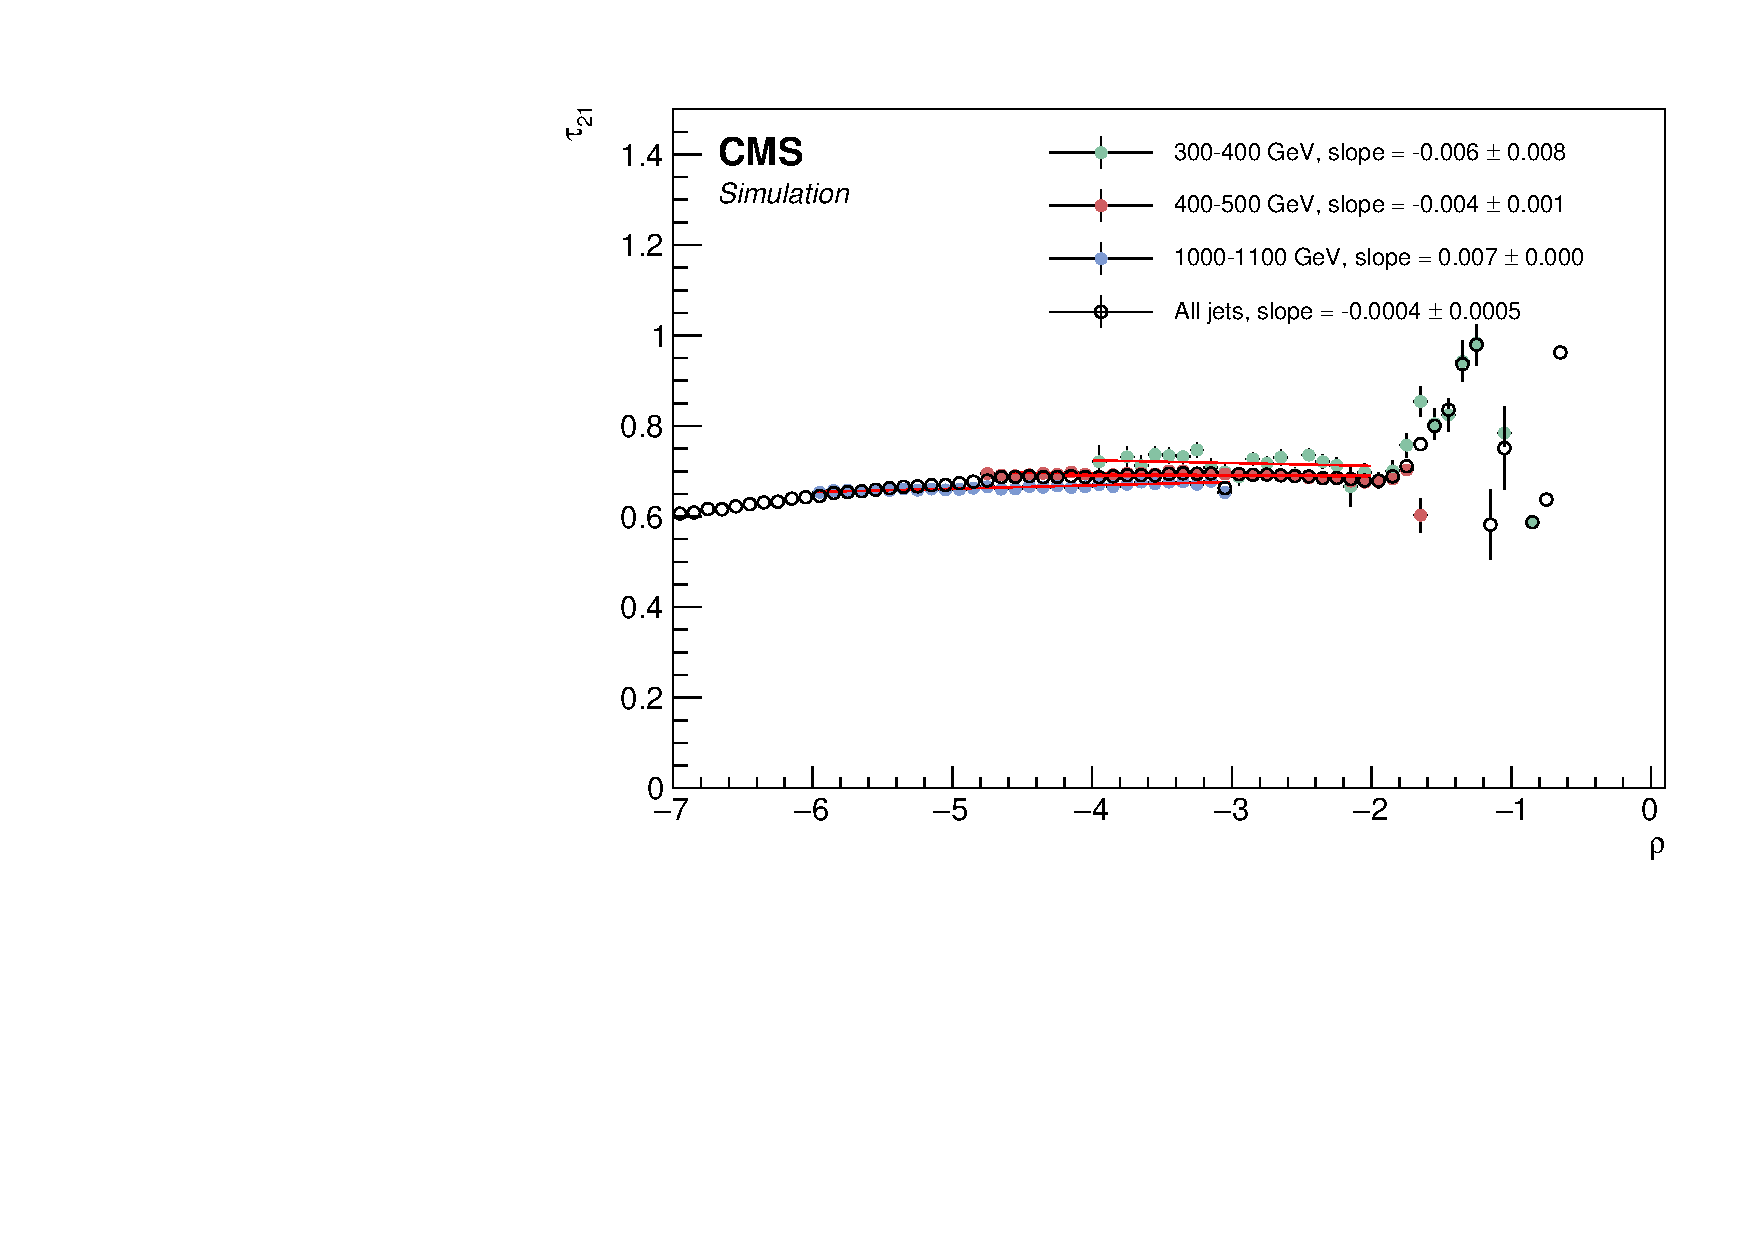
\includegraphics[width=0.45\textwidth]{figures/analysis/search3/AN-17-303/vtag/rho_pythia_FullSel_rhoClosure.pdf}
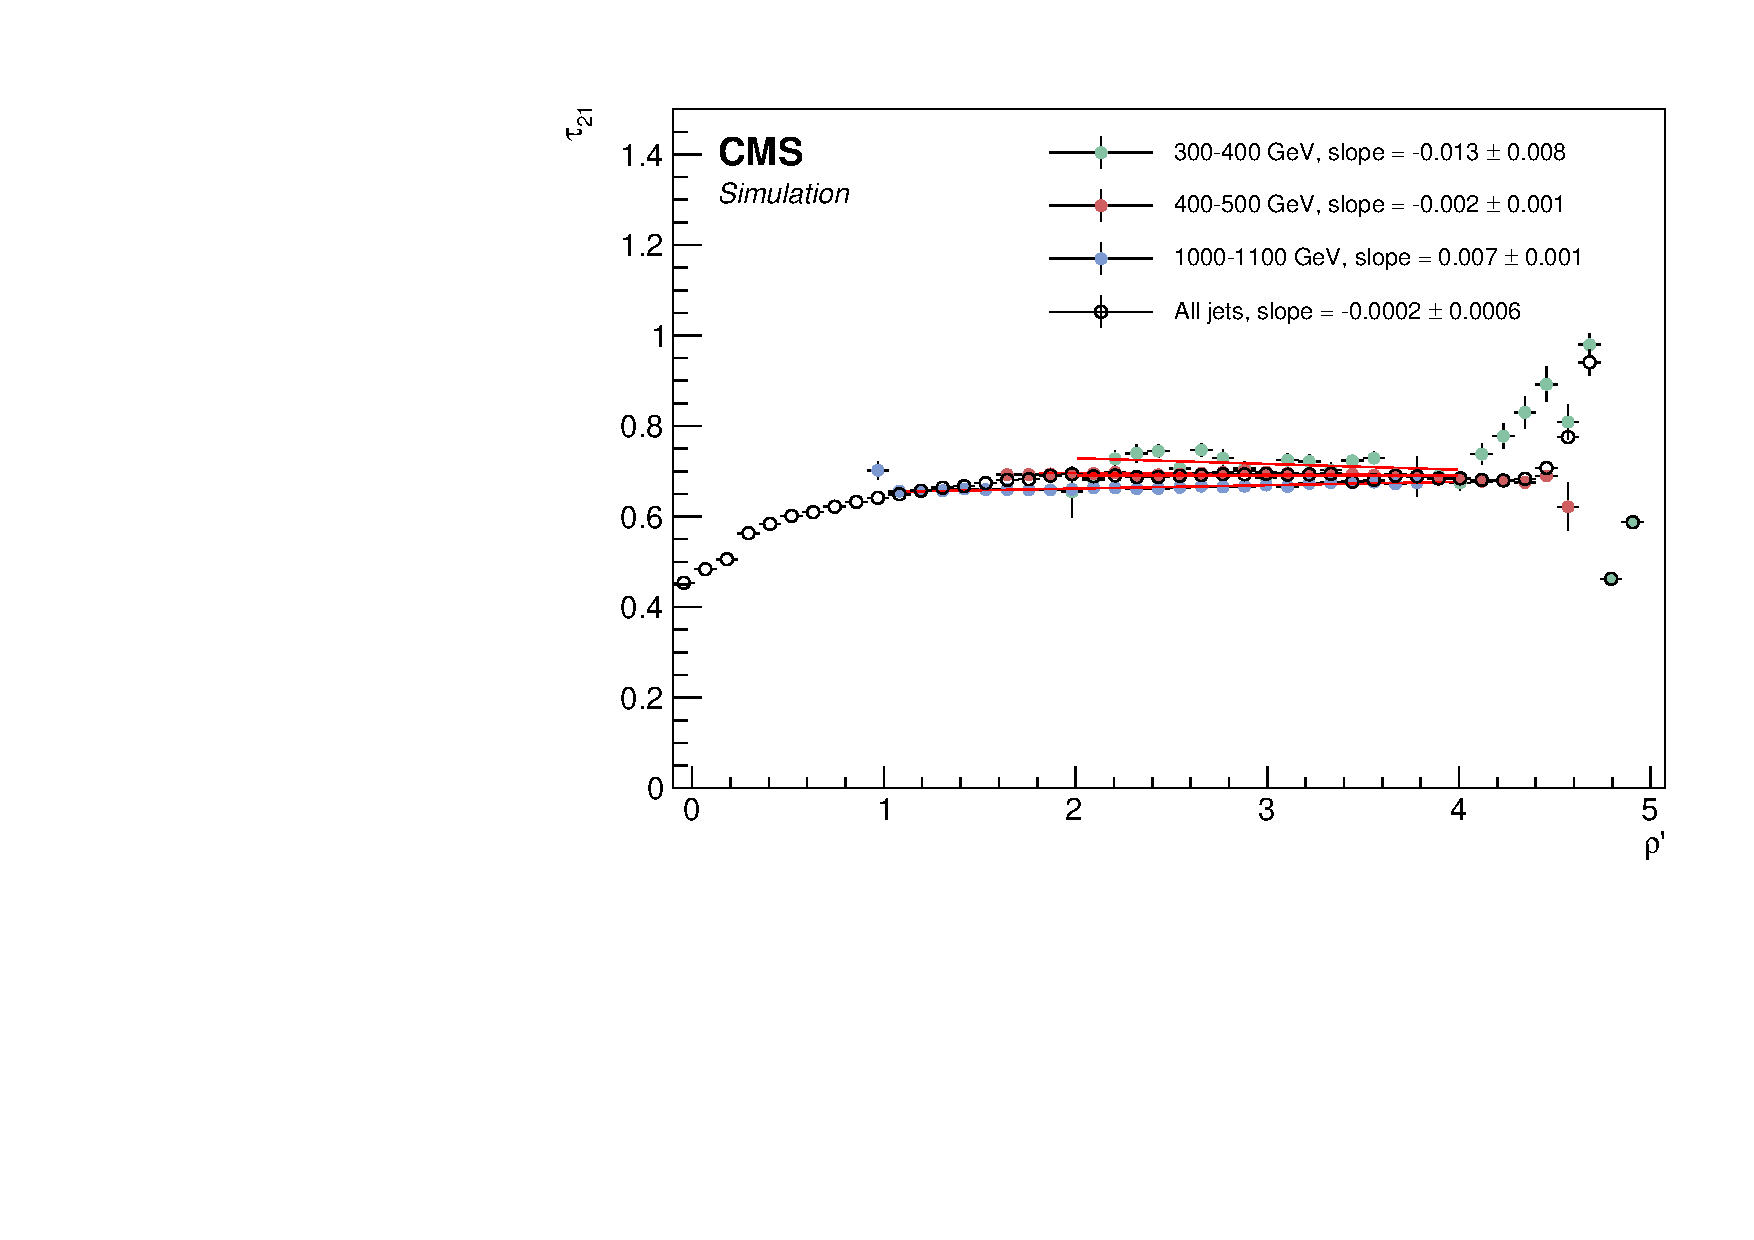
\includegraphics[width=0.45\textwidth]{figures/analysis/search3/AN-17-303/vtag/rho_pythia_FullSel_rhoPrimeClosure.pdf}
\end{tabular}
\caption{Profile distributions of $\tau_{21}^{DDT}$ as a function of $\rho' = log(m^2/p_T/\mu)$, where $\mu$ = 1 GeV.}
\label{fig:rhoClosure}
\end{figure}
Which selections on \ddt to be used are chosen in the following way. First, we check which \ddt selection corresponds to the highest Punzi significance as a function of the resonance mass for different signal samples, as shown in Figure~\ref{fig:punzi}. All other analysis selections, including a selection on the groomed-jet mass of $\unit{55} < m_{sd} < \unit{215}{\GeV}$, have been applied.
\begin{figure}[h!]
\centering
\begin{tabular}{cc}
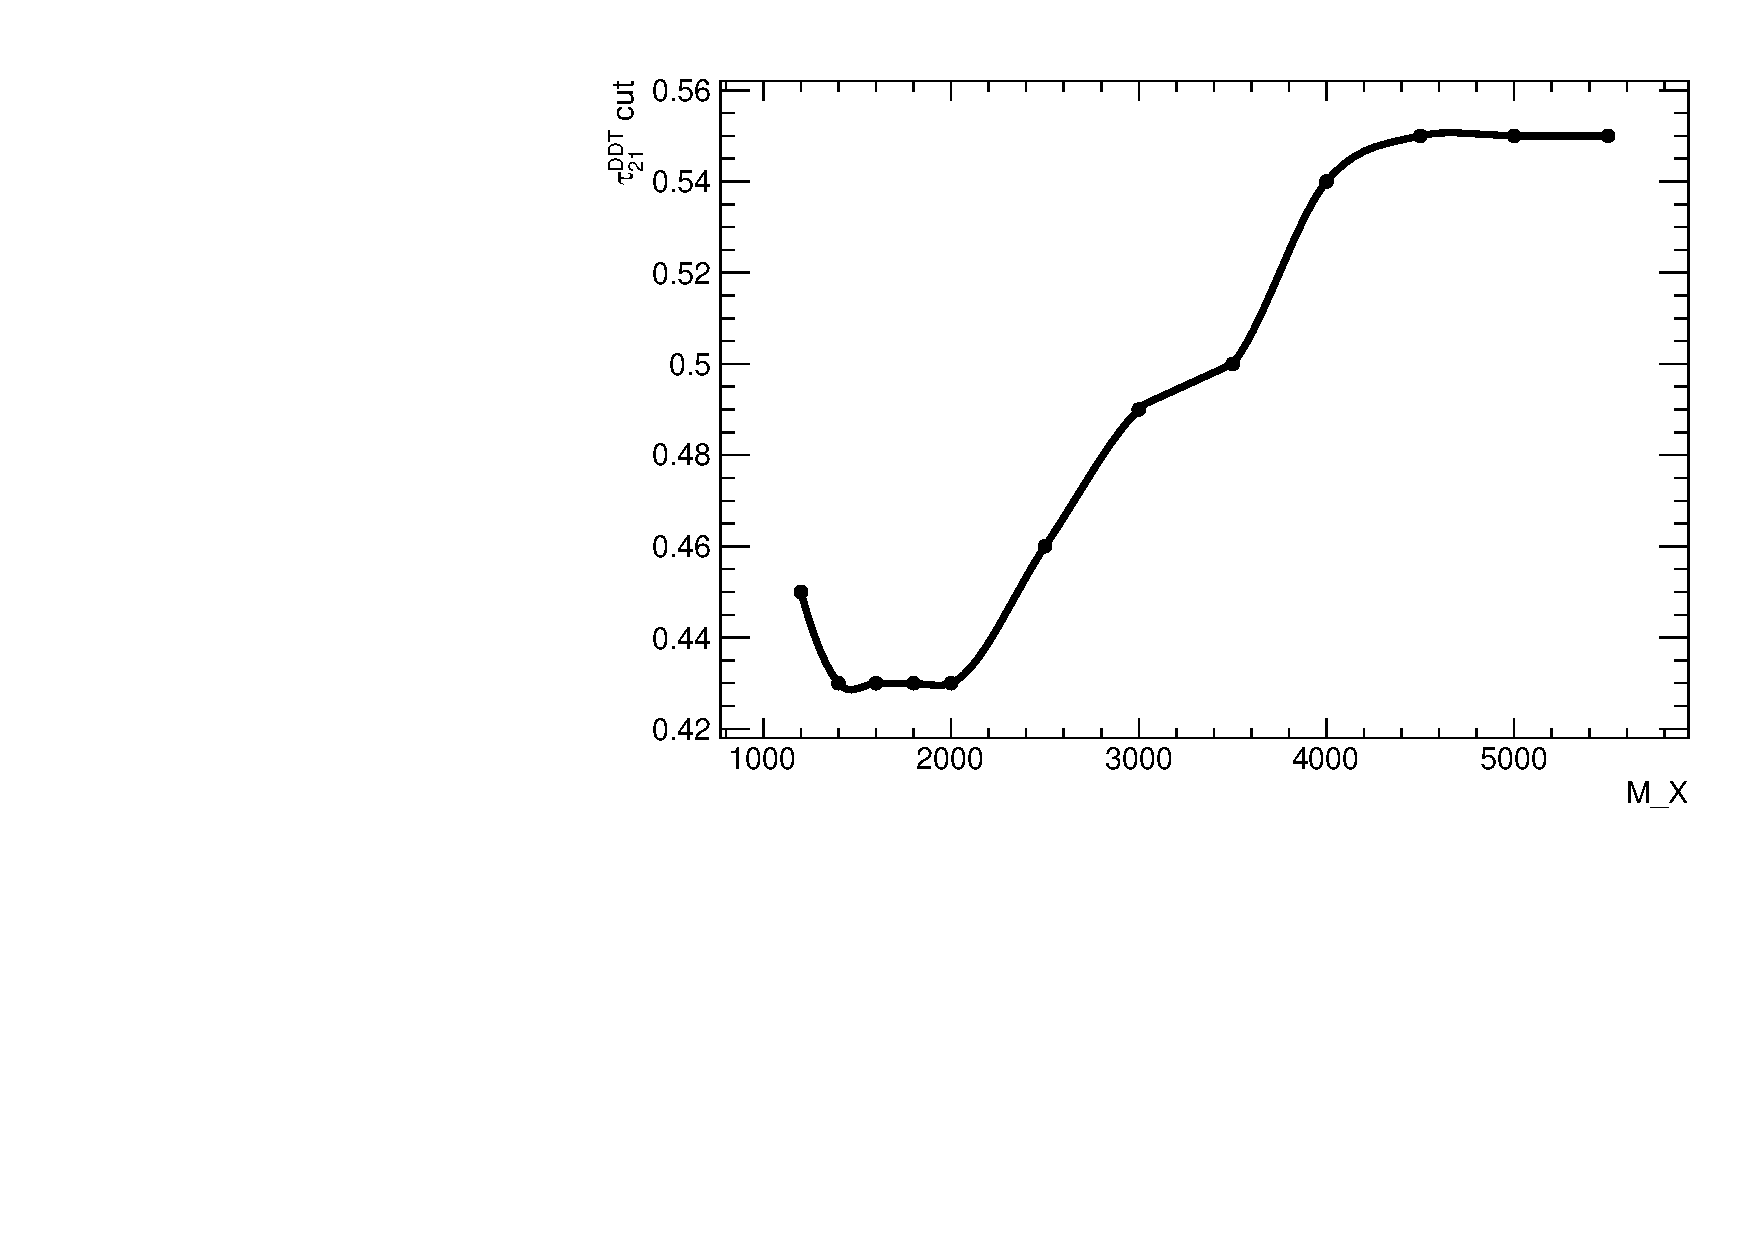
\includegraphics[width=0.45\textwidth]{figures/analysis/search3/AN-17-303/vtag/tau21ddt_punzi_BulkGravToZZToZhadZhad.pdf}
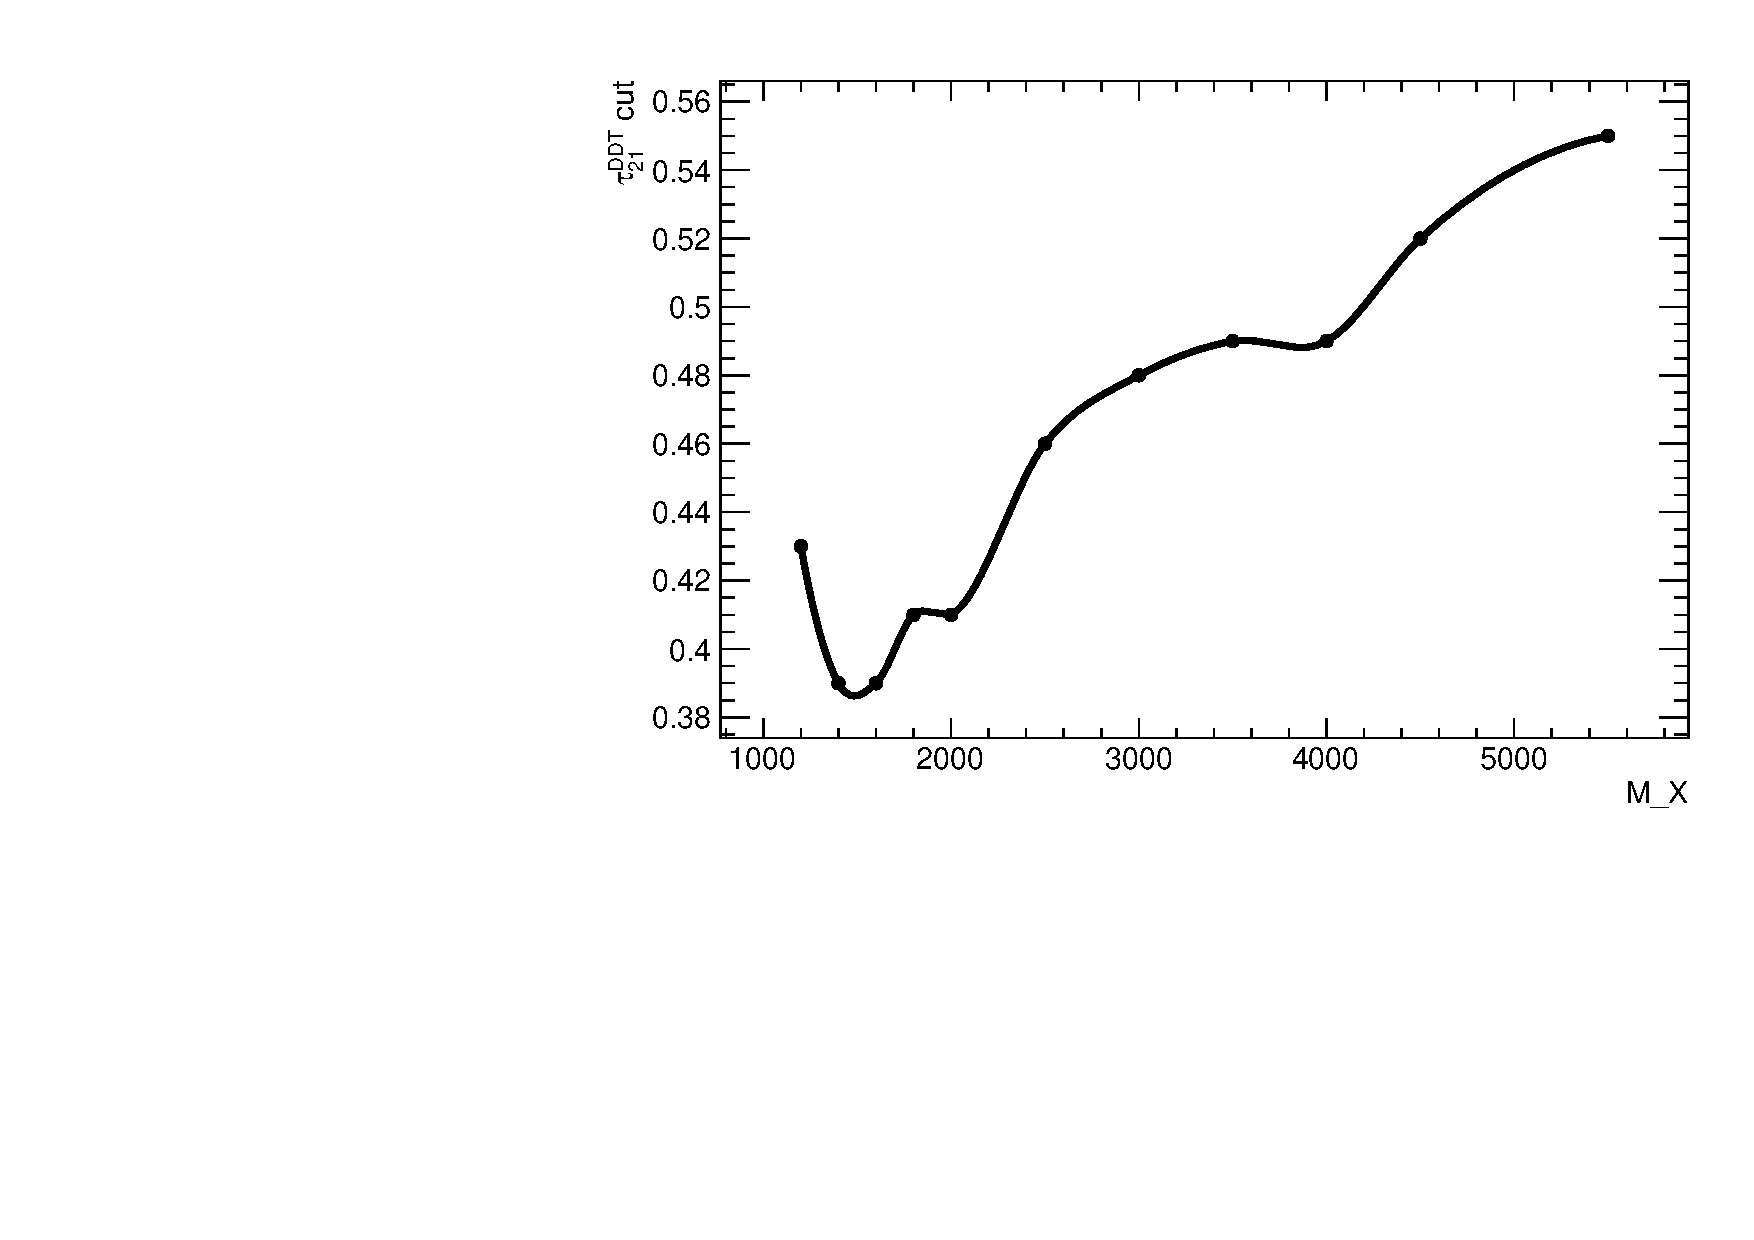
\includegraphics[width=0.45\textwidth]{figures/analysis/search3/AN-17-303/vtag/tau21ddt_punzi_BulkGravToWW.pdf}
\end{tabular}
\caption{The $\tau_{21}^{DDT}$ cut corresponding to the highest Punzi significance for a given signal resonance mass, here for a Bulk $G\rightarrow WW$ (left) and a Bulk $G\rightarrow ZZ$ (right) signal.}
\label{fig:punzi}
\end{figure}
The cut maximizing the Punzi significance at lower resonance mass, where the background is highest, is chosen as the "high-purity" (HP) working point.
This corresponds to $\tau_{21}^{DDT} \leq 0.43$. We then proceed by finding which selections on \ddt contains at least 95\% of the signal, and out of those select the one that optimizes the Punzi significance. This is found to be $0.43<\tau_{21}^{DDT}\leq0.79$, and is classified as the low purity (LP) category. The purpose of this category is to enhance the overall sensitivity of the analysis, especially where the background is low.\par
Figure~\ref{fig:searchIII:roc} shows the performance of $\tau_{21}$ and $\tau_{21}^{DDT}$ (2016 and 2017 tune) in the background-signal efficiency plane (top). We observe a significant gain in signal efficiency at a fixed mistag rate with the decorrelated taggers, when not using a tight jet groomed mass selection (recall: a window of $\unit{55}{\GeV} < M_{SD} < \unit{215}{\GeV}$ is used in this analysis). That is because we are taking advantage of far more information when computing the DDT: subjettiness, and the ratio of jet groomed mass and momentum. All these have a distribution which is different between quark/gluon jets and W-jets, leading to a larger separation between signal and background, as can be seen when comparing the distributions of the different taggers in the left plot of Figure~\ref{fig:searchIII:m2pt}. The distribution of $log(m_{SD}^2/p_T)$ is shown on the right in Figure~\ref{fig:searchIII:m2pt}, and it it clear that the variable adds discriminating power.
\begin{figure}[h!]
\centering
\begin{tabular}{cc}
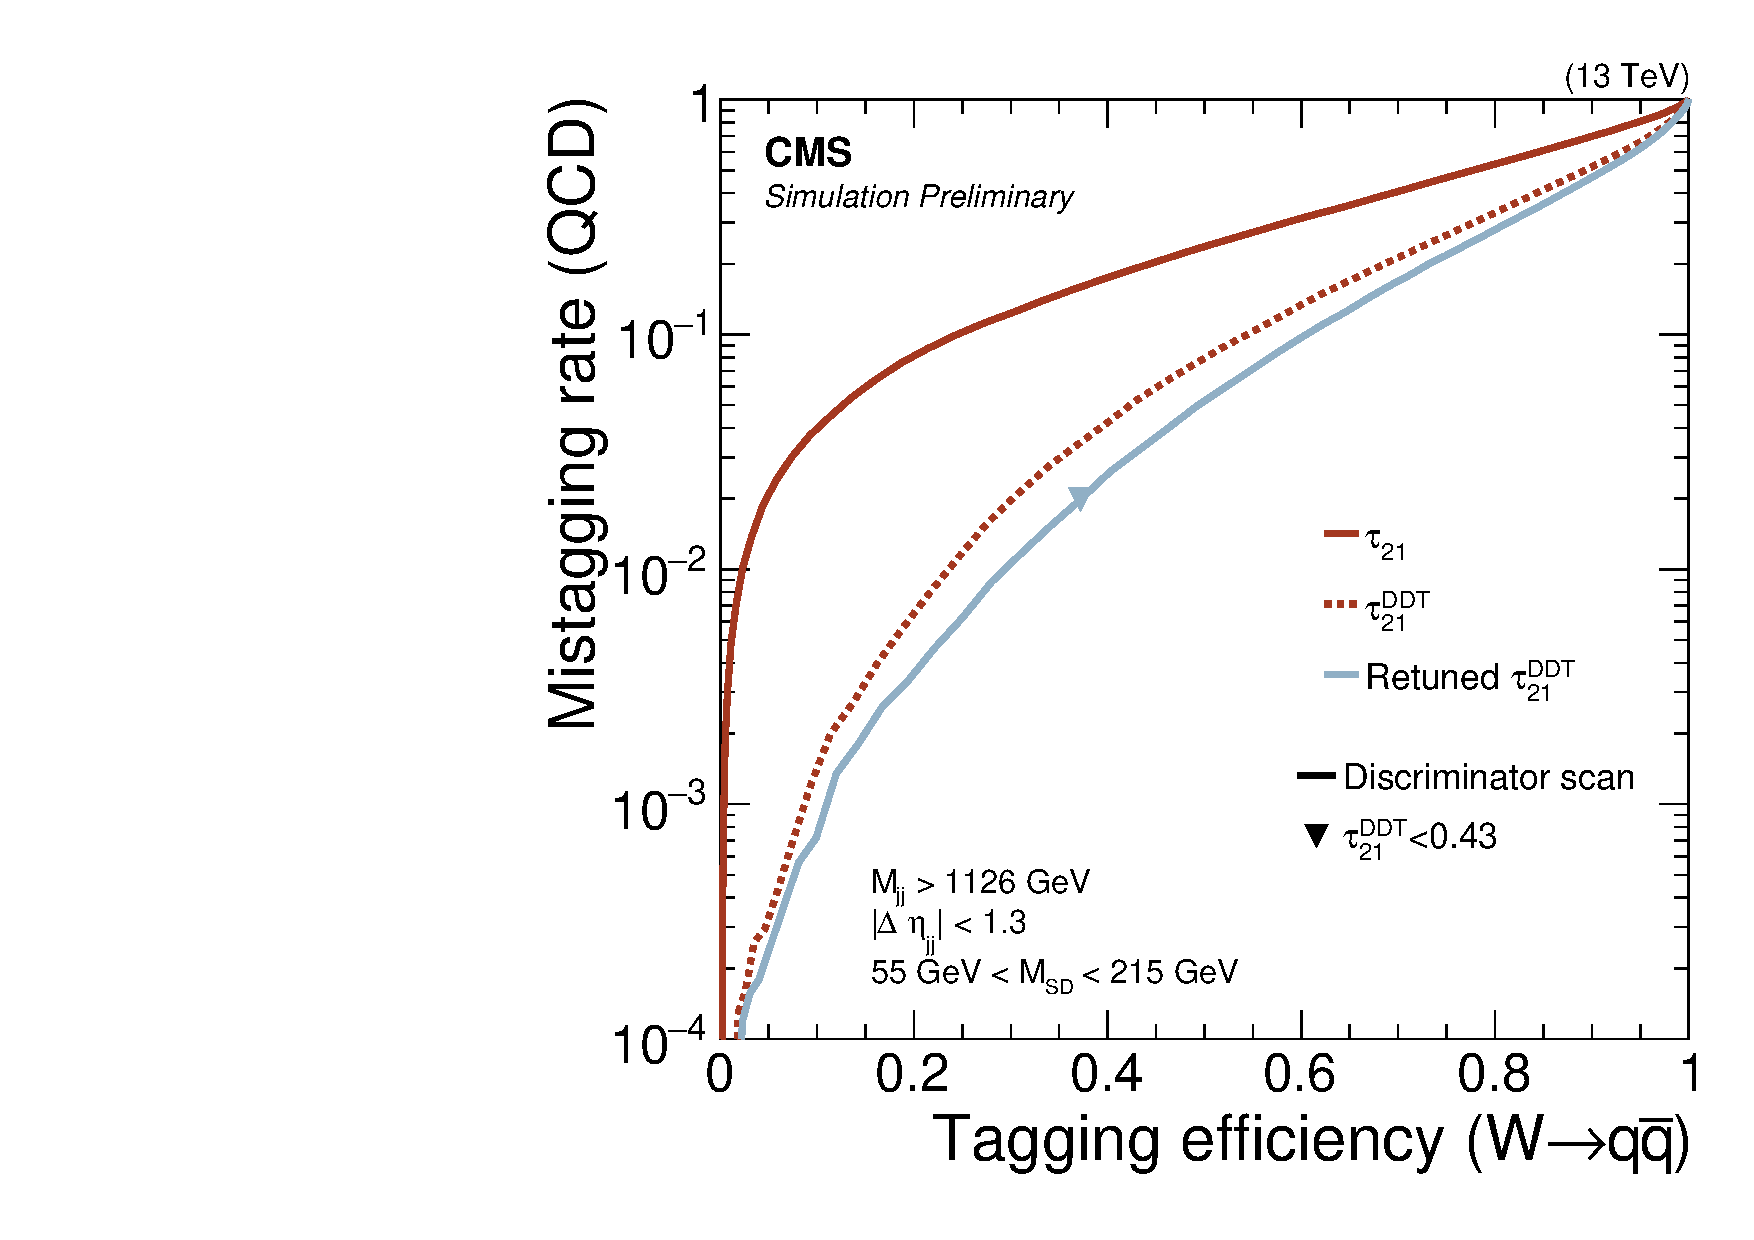
\includegraphics[width=0.45\textwidth]{figures/analysis/search3/AN-17-303/vtag/rocTau21s.pdf}
\end{tabular}
\caption{Performance of $\tau_{21}$ and $\tau_{21}^{DDT}$ (2016 and 2017 tune) in the background-signal efficiency plane.}
\label{fig:searchIII:roc}
\end{figure}
\begin{figure}[h!]
\centering
\begin{tabular}{cc}
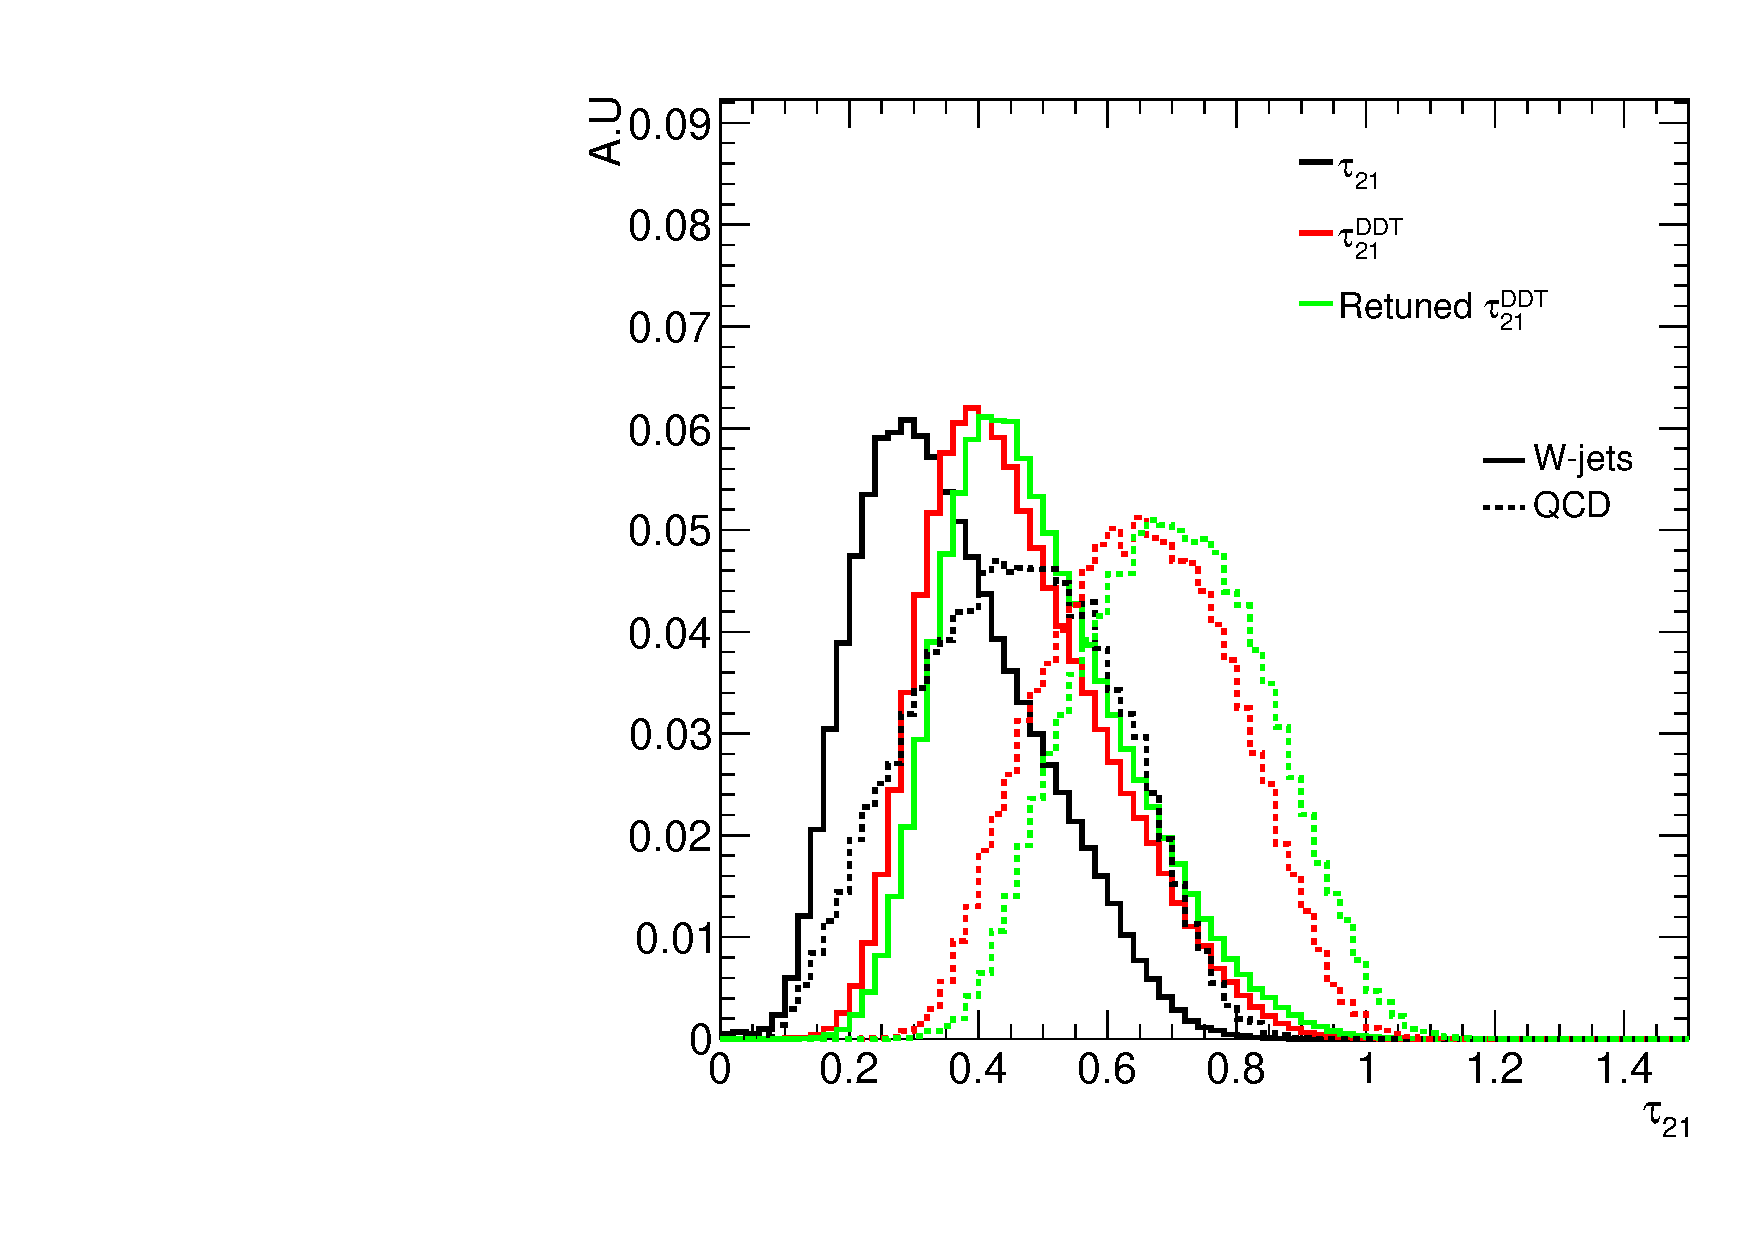
\includegraphics[width=0.45\textwidth]{figures/analysis/search3/AN-17-303/vtag/compare_tau21s.pdf}
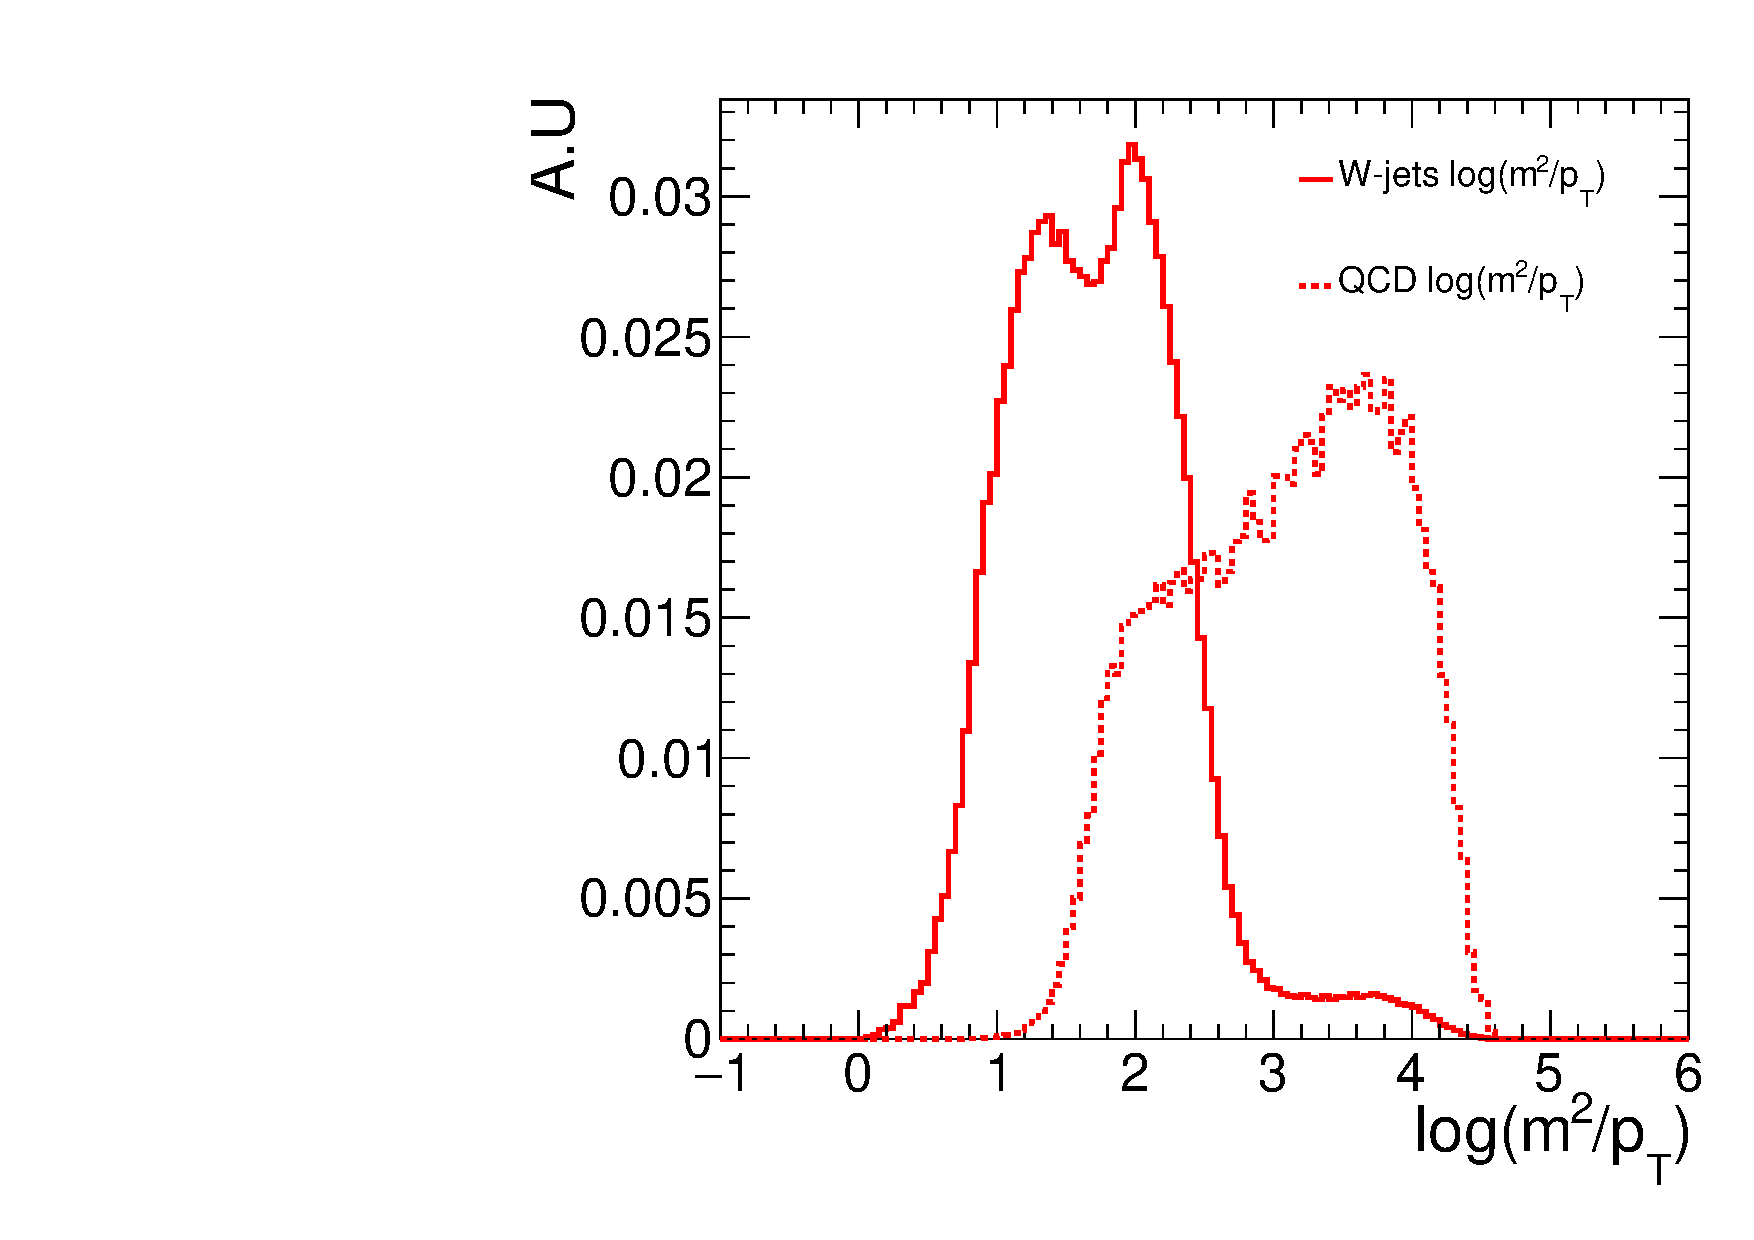
\includegraphics[width=0.45\textwidth]{figures/analysis/search3/AN-17-303/vtag/logm2pt.pdf}
\end{tabular}
\caption{Distribution of $\tau_{21}$ and $\tau_{21}^{DDT}$ with the old and the new tune (left) and comparison of $log(m^2/p_T)$ for signal and background jets (right).}
\label{fig:searchIII:m2pt}
\end{figure}\noindent 
In addition to cutting on $\tau_{21}^{DDT}$, a selection on $\rho = log(m^2/p_T^2) < -1.8 $ is applied. This is in order to avoid configurations where the jet mass is high, but the jet transverse momentum is low. In these cases, the AK8 cone size is too small to contain the full jet, affecting both the jet mass resolution and the \ddt tagging efficiency. These edge effects are difficult to model in simulation and we therefore avoid this region in the following. Figure~\ref{fig:rhoDDT} shows the profile distribution of \ddt versus $\rho$ for QCD jets, where a clear deviation from the observed linear spectra is observed above a $\rho$ of -1.8.
\begin{figure}[h!]
\centering
\begin{tabular}{cc}
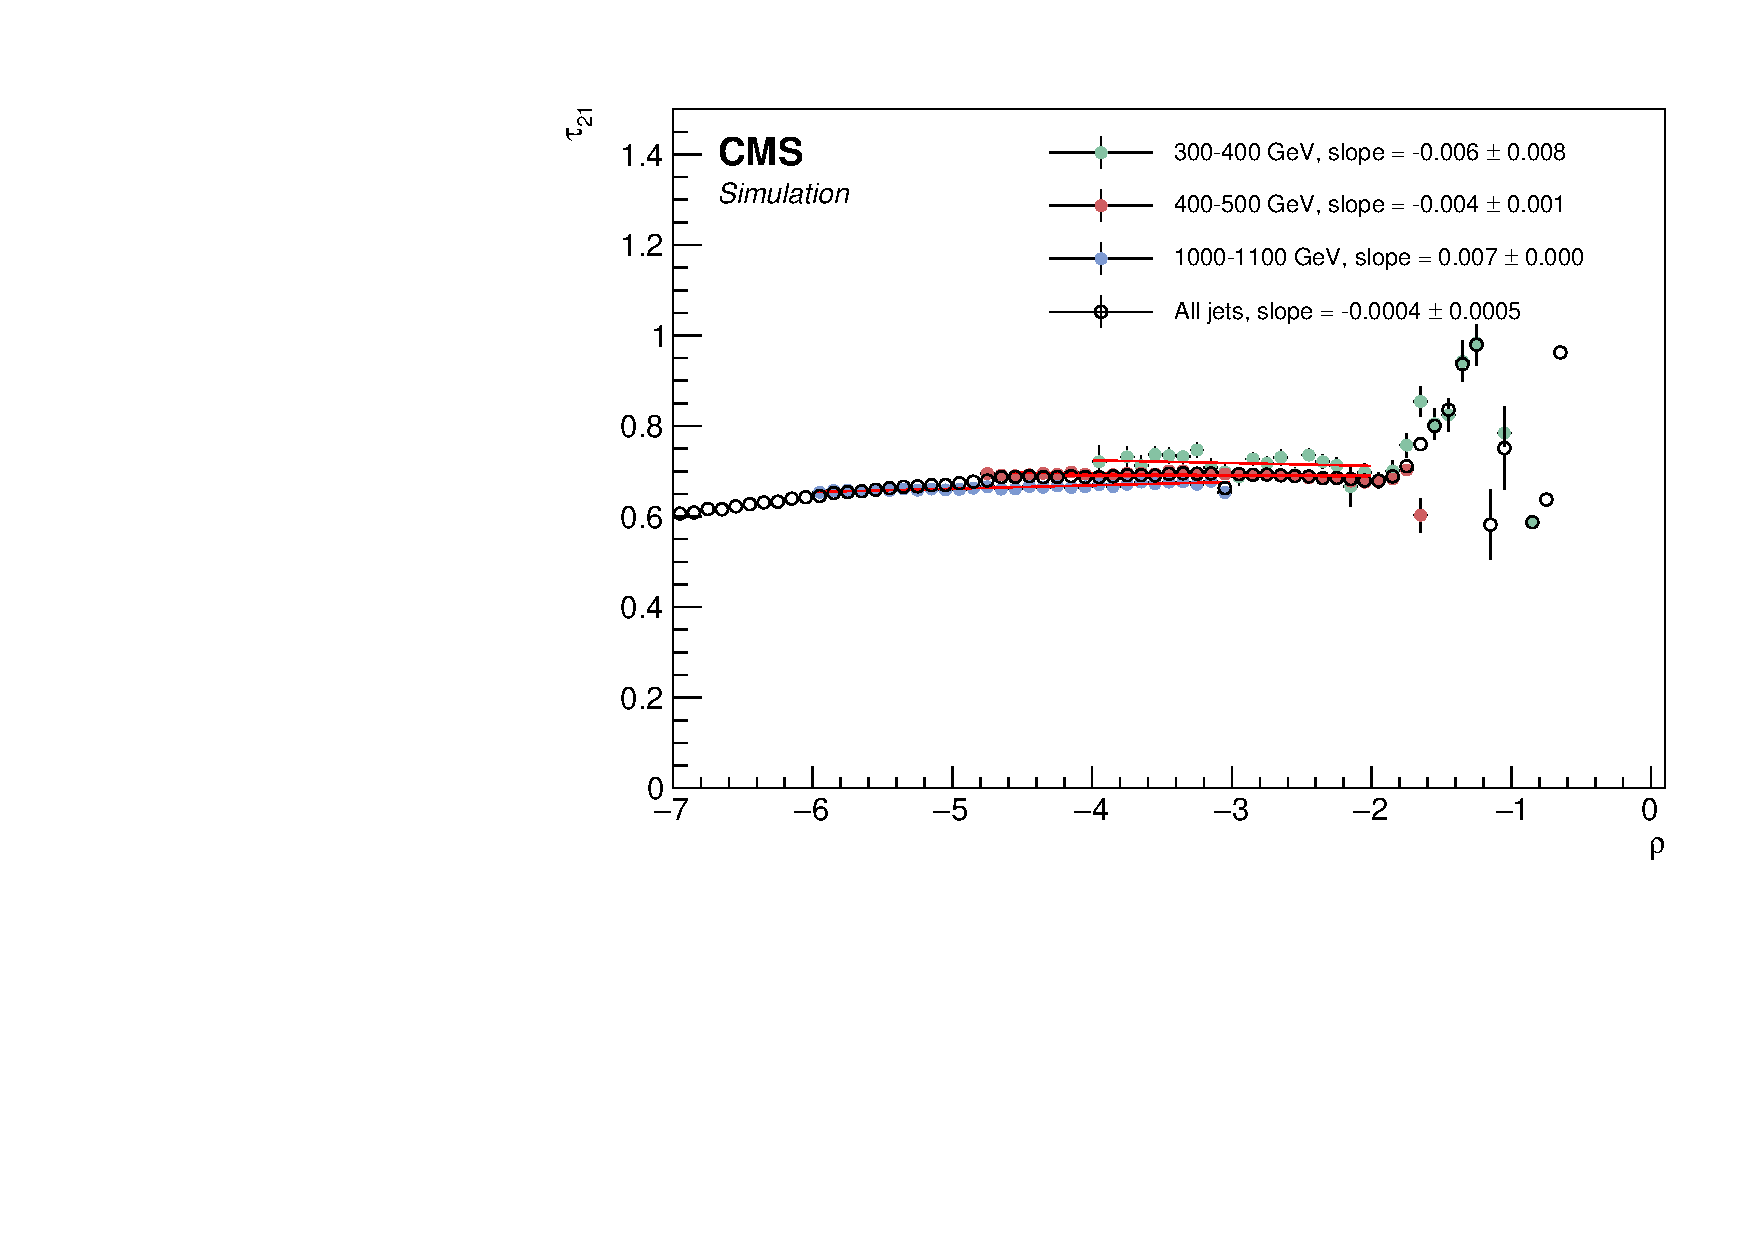
\includegraphics[width=0.45\textwidth]{figures/analysis/search3/AN-17-303/vtag/rho_pythia_FullSel_rhoClosure.pdf}
\end{tabular}
\caption{Profile distributions of $\tau_{21}^{DDT}$ as a function of $\rho = log(m^2/p_T^2)$, where $\mu$ = 1 GeV. The DDT breaks down above $\rho=-1.8$. }
\label{fig:rhoDDT}
\end{figure}
 Note that this has a negligible effect on signal jets, which mainly peak around 80 GeV and have a high jet transverse momenta.
Figure~\ref{fig:wtagCP} shows the distributions of the PUPPI softdrop jet mass, the \ddt, and the \nsubj variable for simulation and for data. The softdrop jet mass in the signal distribution peaks nicely around the W mass, while the multijets background spectrum is peaked at lower softdrop masses.
\begin{figure}[h!]
\centering
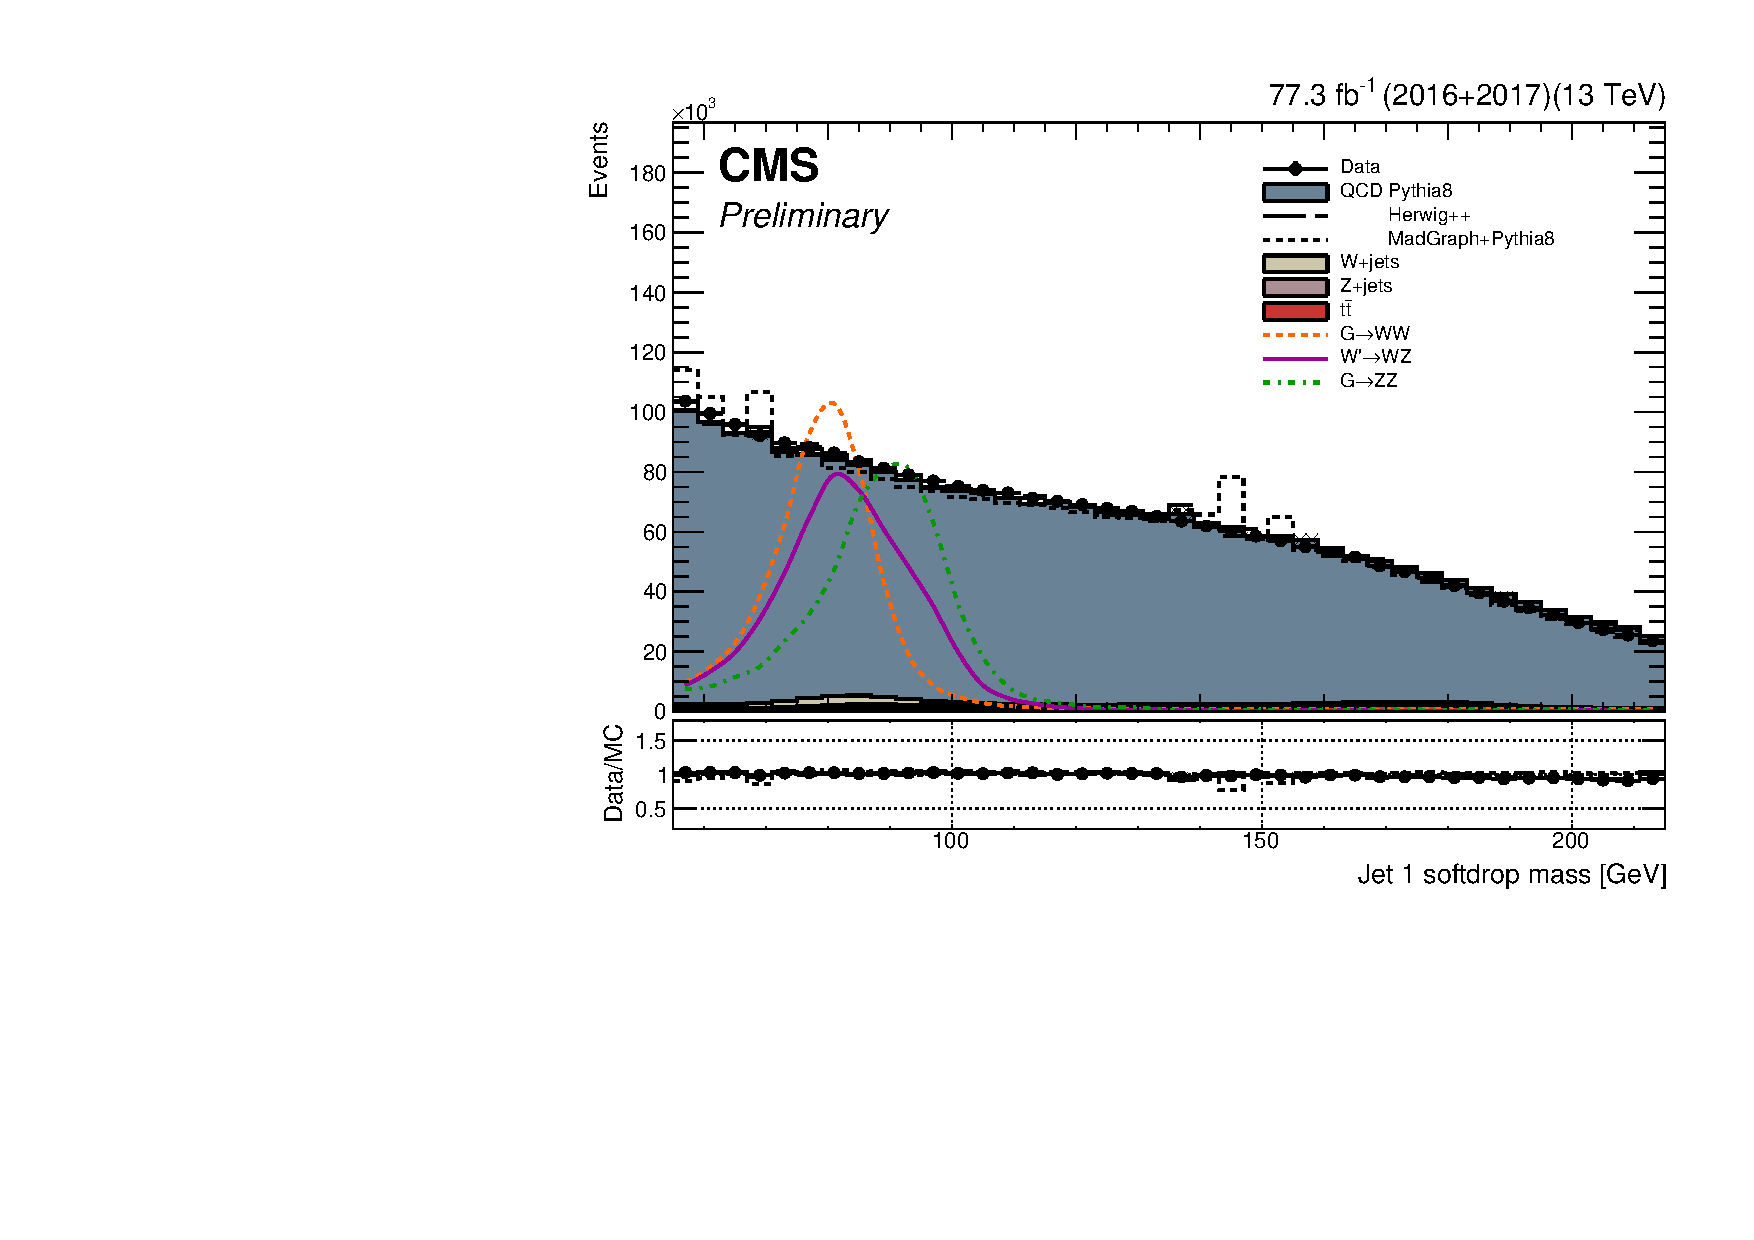
\includegraphics[width=0.450\textwidth]{figures/analysis/search3/B2G-18-002/looseSel_Jet_1_softdrop_mass.pdf}
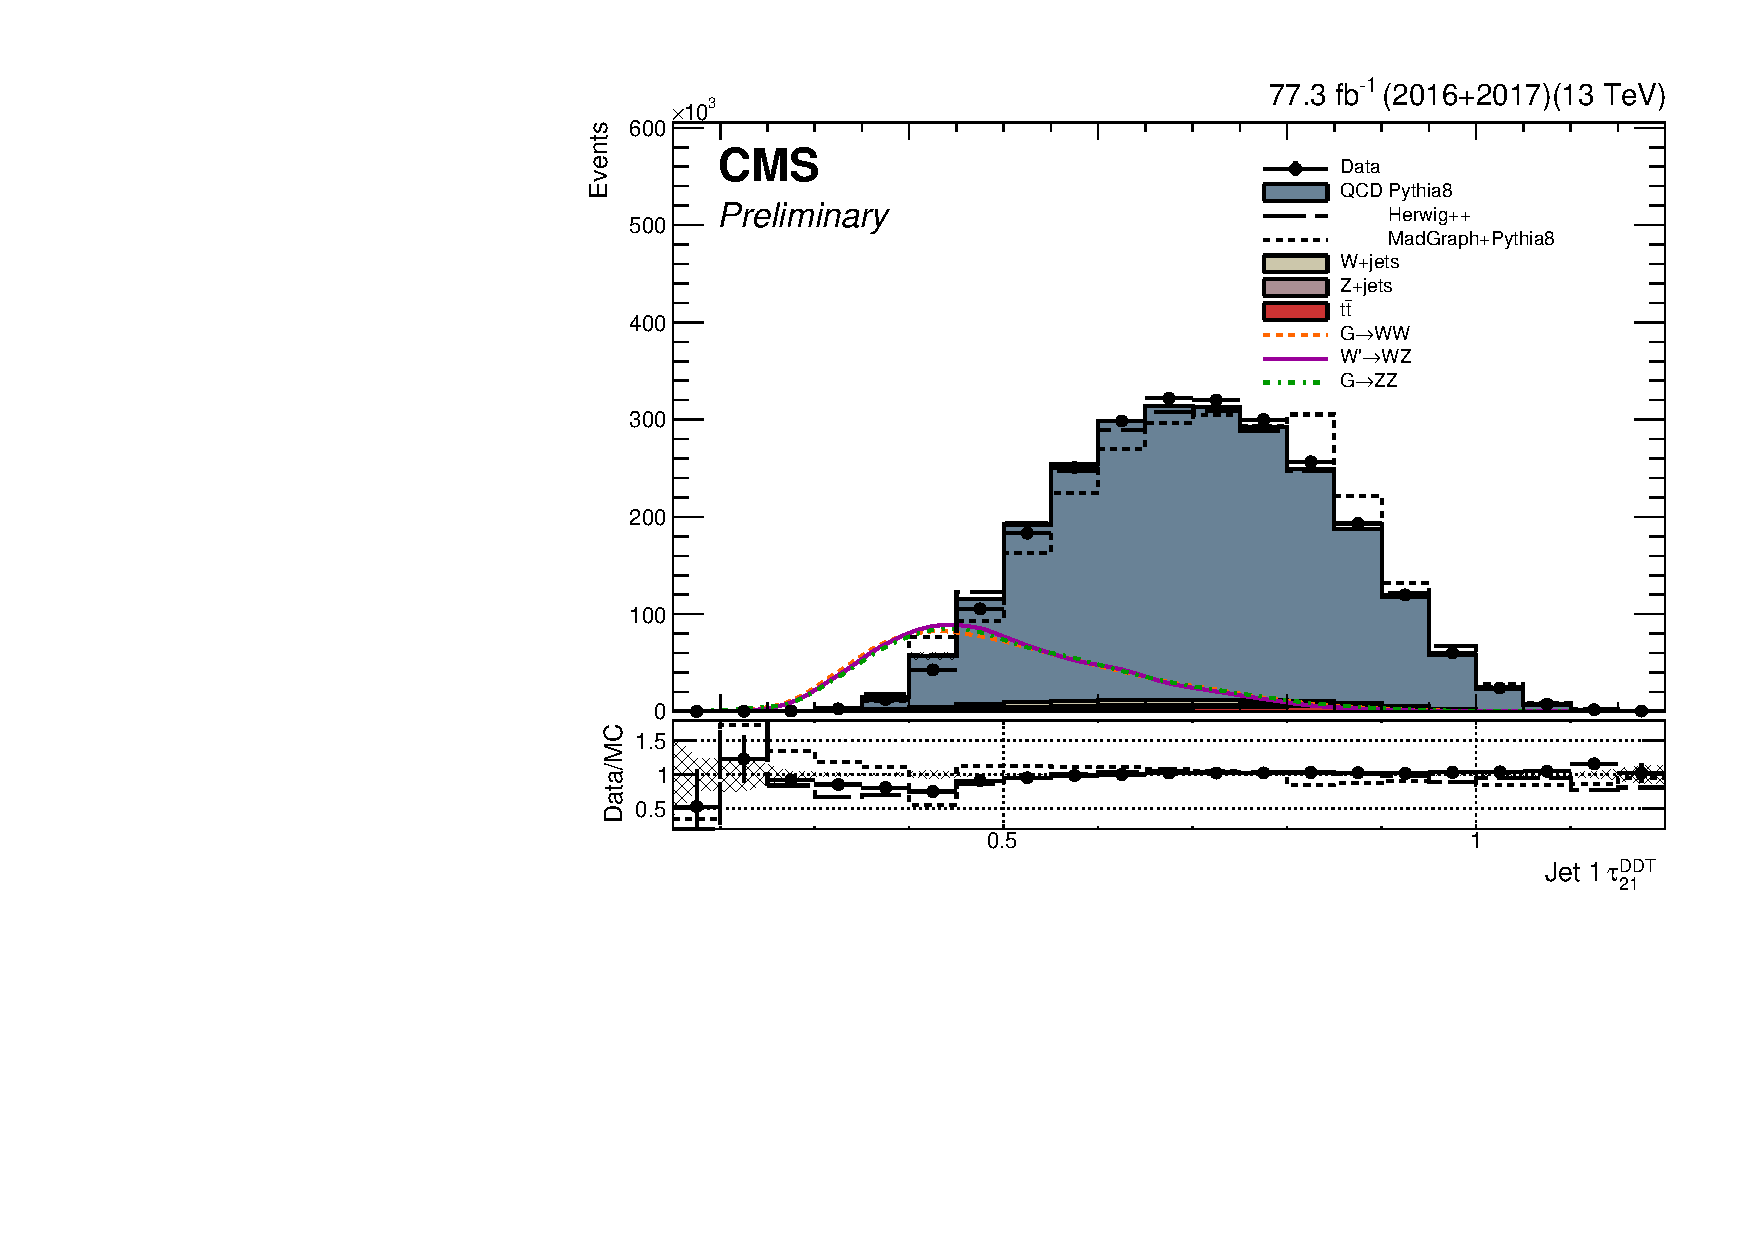
\includegraphics[width=0.450\textwidth]{figures/analysis/search3/B2G-18-002/looseSel_Jet_1_DDT.pdf}\\
\caption{The softdrop jet mass (left) and $\tau_{21}^{DDT}$ (right) distribution in data and in simulation. Signal is scaled by an arbitrary number.}
\label{fig:wtagCP}
\end{figure}
\clearpage
\subsection{Data to simulation scale factors}
\label{sec:searchIII:wtagSF}
Following what was done in Section~\ref{sec:searchI:vtag} and~\ref{sec:searchII:wtagsf}, we derive W-tagging scale factors in order to correct the efficiency in MC of the selection on \ddt, by estimating the ratio of the selection efficiencies in data and in simulation. The softdrop jet mass range is fitted from 55 to 215 \GeV, and the two categories of purity are:
\begin{itemize}
\itemsep0em
  \item pass region: $0 <  \ddt \leq 0.43 \sim$ high-purity,
  \item fail region: $0.43 < \nsubj \leq 0.79 \sim$ low purity.
\end{itemize}
The obtained scale factors, jet-mass scale and resolution together with their statistical uncertainty are listed in Tables~\ref{tab:wsf16} and~\ref{tab:wsf} for 2016 and 2017 data, respectively. The corresponding simultaneous fits are shown in Figure~\ref{fig:simFit}. The W-tagging efficiency in this region is lower than what is expected for signal jets, around 7\% compared to 35\%. This is expected as the measurement in \ttbar is dominated by W-jets with a \PT of around 200\GeV, just where the W decay products merge into a single jet, whereas the signal jets mostly have a transverse momentum above 600\GeV. The signal efficiency for $\nsubj^{DDT}$ increases at a function of jet \PT, as can be seen from Figure~\ref{fig:SignalYields}, whereas the background efficiency is flat by design. In addition to the statistical uncertainty, two systematic uncertainties are evaluated: one due to generator differences and one due to NNLO corrections. The former is evaluated by comparing the resulting scale factors when using \ttbar simulation produced with different generators. The latter is evaluated by comparing the extracted efficiency with and without top-\PT reweighting. This weight is derived from data in order to better describe the observed \PT distribution in \ttbar and is calculated for each top jet as $w=\exp^{0.0615-0.0005*p_{T,top}}$. The W tagging scale factors, jet mass scale, and jet mass resolution, with their total uncertainty after adding systematics, are listed in Table~\ref{tab:wsf_total}. As before, the scale factor is used to scale the signal yield and the jet mass scale and resolution are used to smear the MC. The difference in jet mass scale between data and simulation is around 2\%, and the jet mass resolution scale factor is roughly 8\%.
 \begin{table}[h!]
    \centering
    \begin{tabular}{|lccc|}
    \hline
    & m [GeV]           & $\sigma$~[GeV]     & W-tag efficiency\\
    $\tau_{21}^{DDT} < 0.43$ & &&\\ \hline
    \hline
    Data            & 81.999$\pm$ 0.454~GeV   & 7.148 $\pm$ 0.544~GeV & 0.080 $\pm$ 0.008\\
    Simulation      & 80.890$\pm$ 0.160~GeV   & 6.579 $\pm$ 0.149~GeV & 0.085 $\pm$ 0.003\\
    \hline
    Data/simulation & 1.014$\pm$ 0.006       & 1.086 $\pm$ 0.086     & 0.937 $\pm$ 0.094\\
    \hline
    $0.43 < \tau_{21}^{DDT} < 0.79$ & &&\\ \hline
    \hline
    Data            &    &  & 0.920 $\pm$ 0.008\\
    Simulation      &    &  & 0.915 $\pm$ 0.003\\
    \hline
    Data/simulation &    &   & 1.006 $\pm$ 0.009\\
    \hline
    \end{tabular}
     \caption{Jet mass scale, jet mass resolution, and \ddt scale factors, as evaluated in the full 2016 single-muon dataset.}
    \label{tab:wsf16}
 \end{table}
 \begin{table}[htbp]
    \centering
    \begin{tabular}{|lccc|}
    \hline
    & m [GeV]           & $\sigma$~[GeV]     & W-tag efficiency\\
    $\tau_{21}^{DDT} < 0.43$ & &&\\ \hline
    \hline
    Data            & 80.784$\pm$ 0.391~GeV   & 7.694 $\pm$ 0.445~GeV & 0.065 $\pm$ 0.006\\
    Simulation      & 82.208$\pm$ 0.293~GeV   & 7.127 $\pm$ 0.284~GeV & 0.068 $\pm$ 0.005\\
    \hline
    Data/simulation & 0.983$\pm$ 0.006       & 1.080 $\pm$ 0.076     & 0.955 $\pm$ 0.113\\
    \hline
    $0.43 < \tau_{21}^{DDT} < 0.79$ & &&\\ \hline
    \hline
    Data            &    &  & 0.935 $\pm$ 0.006\\
    Simulation      &    &  & 0.932 $\pm$ 0.005\\
    \hline
    Data/simulation &    &   & 1.003 $\pm$ 0.008\\
    \hline
    \end{tabular}
    \caption{Jet mass scale, jet mass resolution, and \ddt scalefactors as evaluated in the full 2017 single-muon dataset.}
    \label{tab:wsf}
 \end{table}
 \begin{figure}[h!]
 \centering
 \begin{tabular}{cc}
 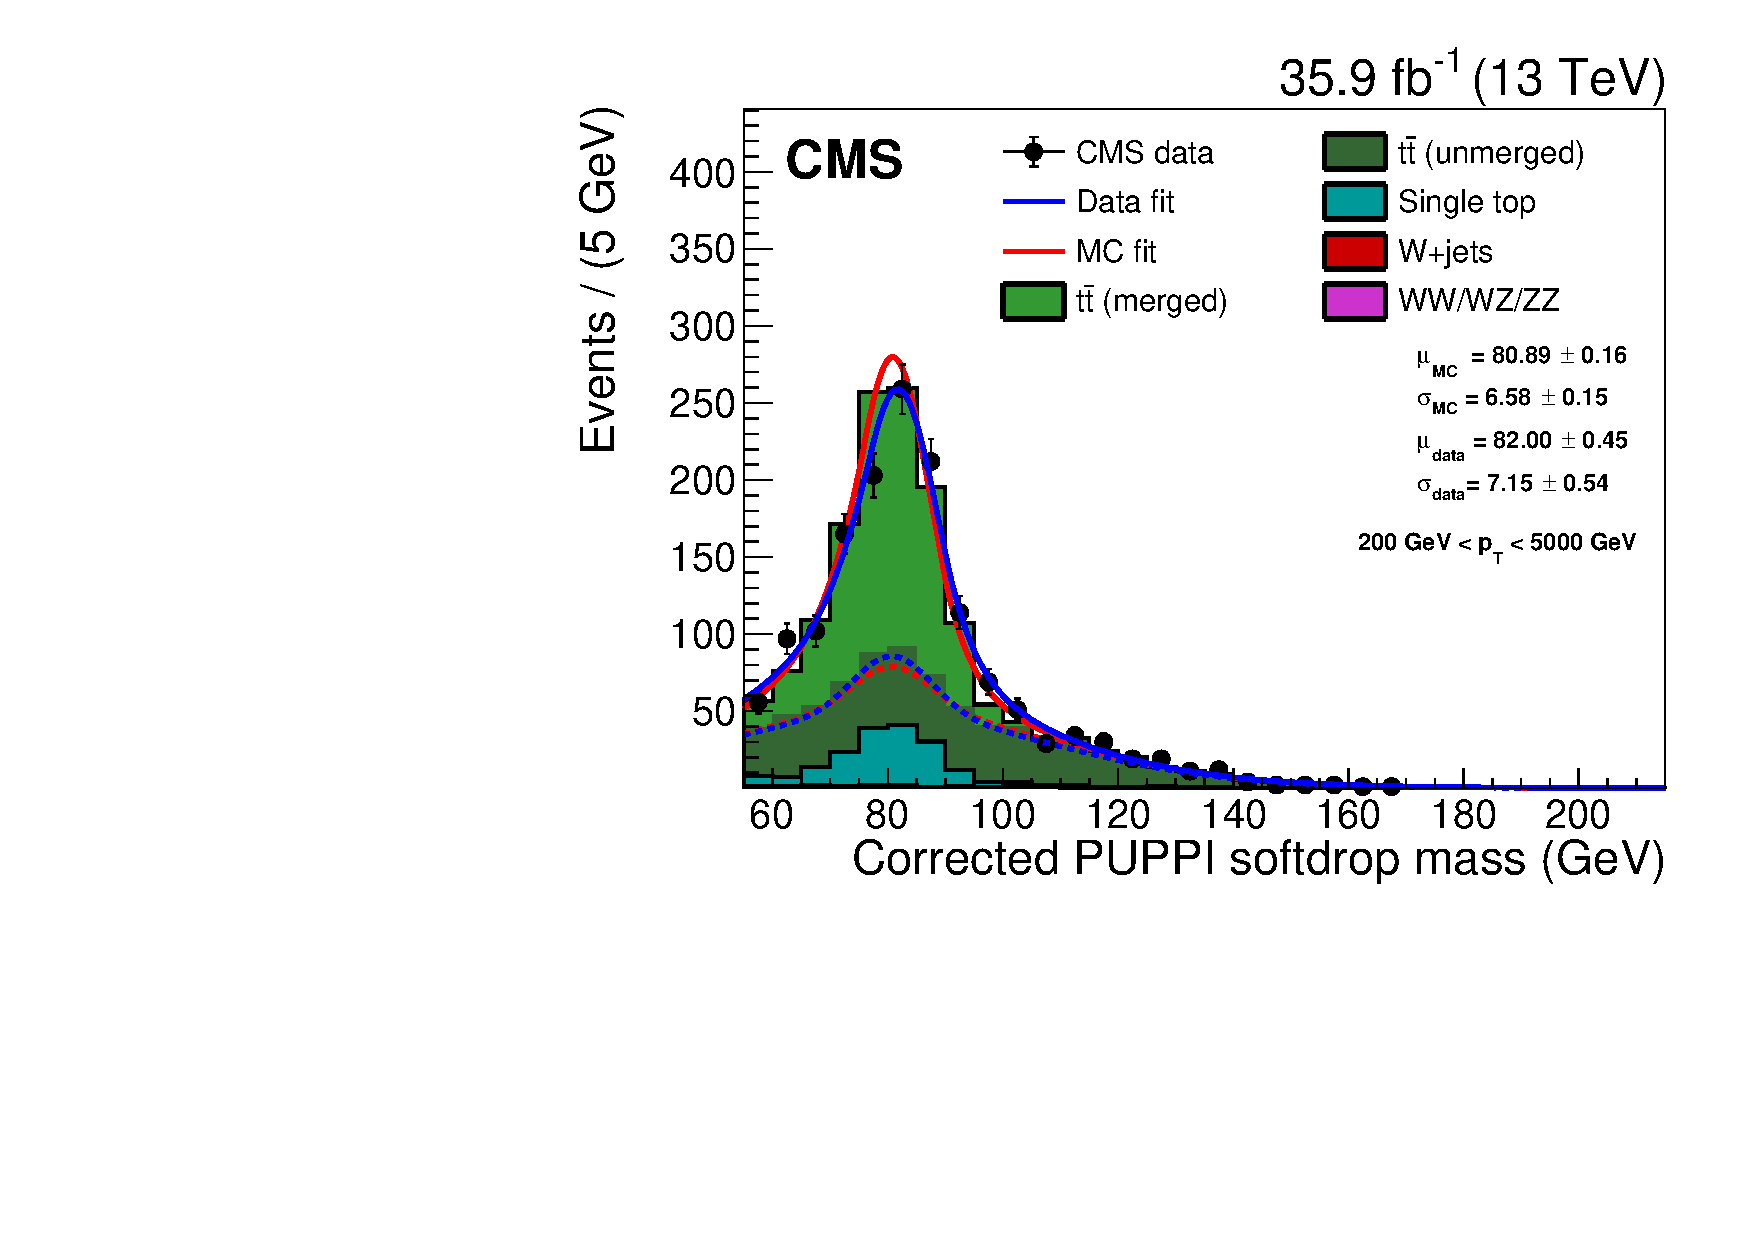
\includegraphics[width=0.49\textwidth]{figures/analysis/search3/AN-17-303/vtag/newddt_2016_pass.pdf}
 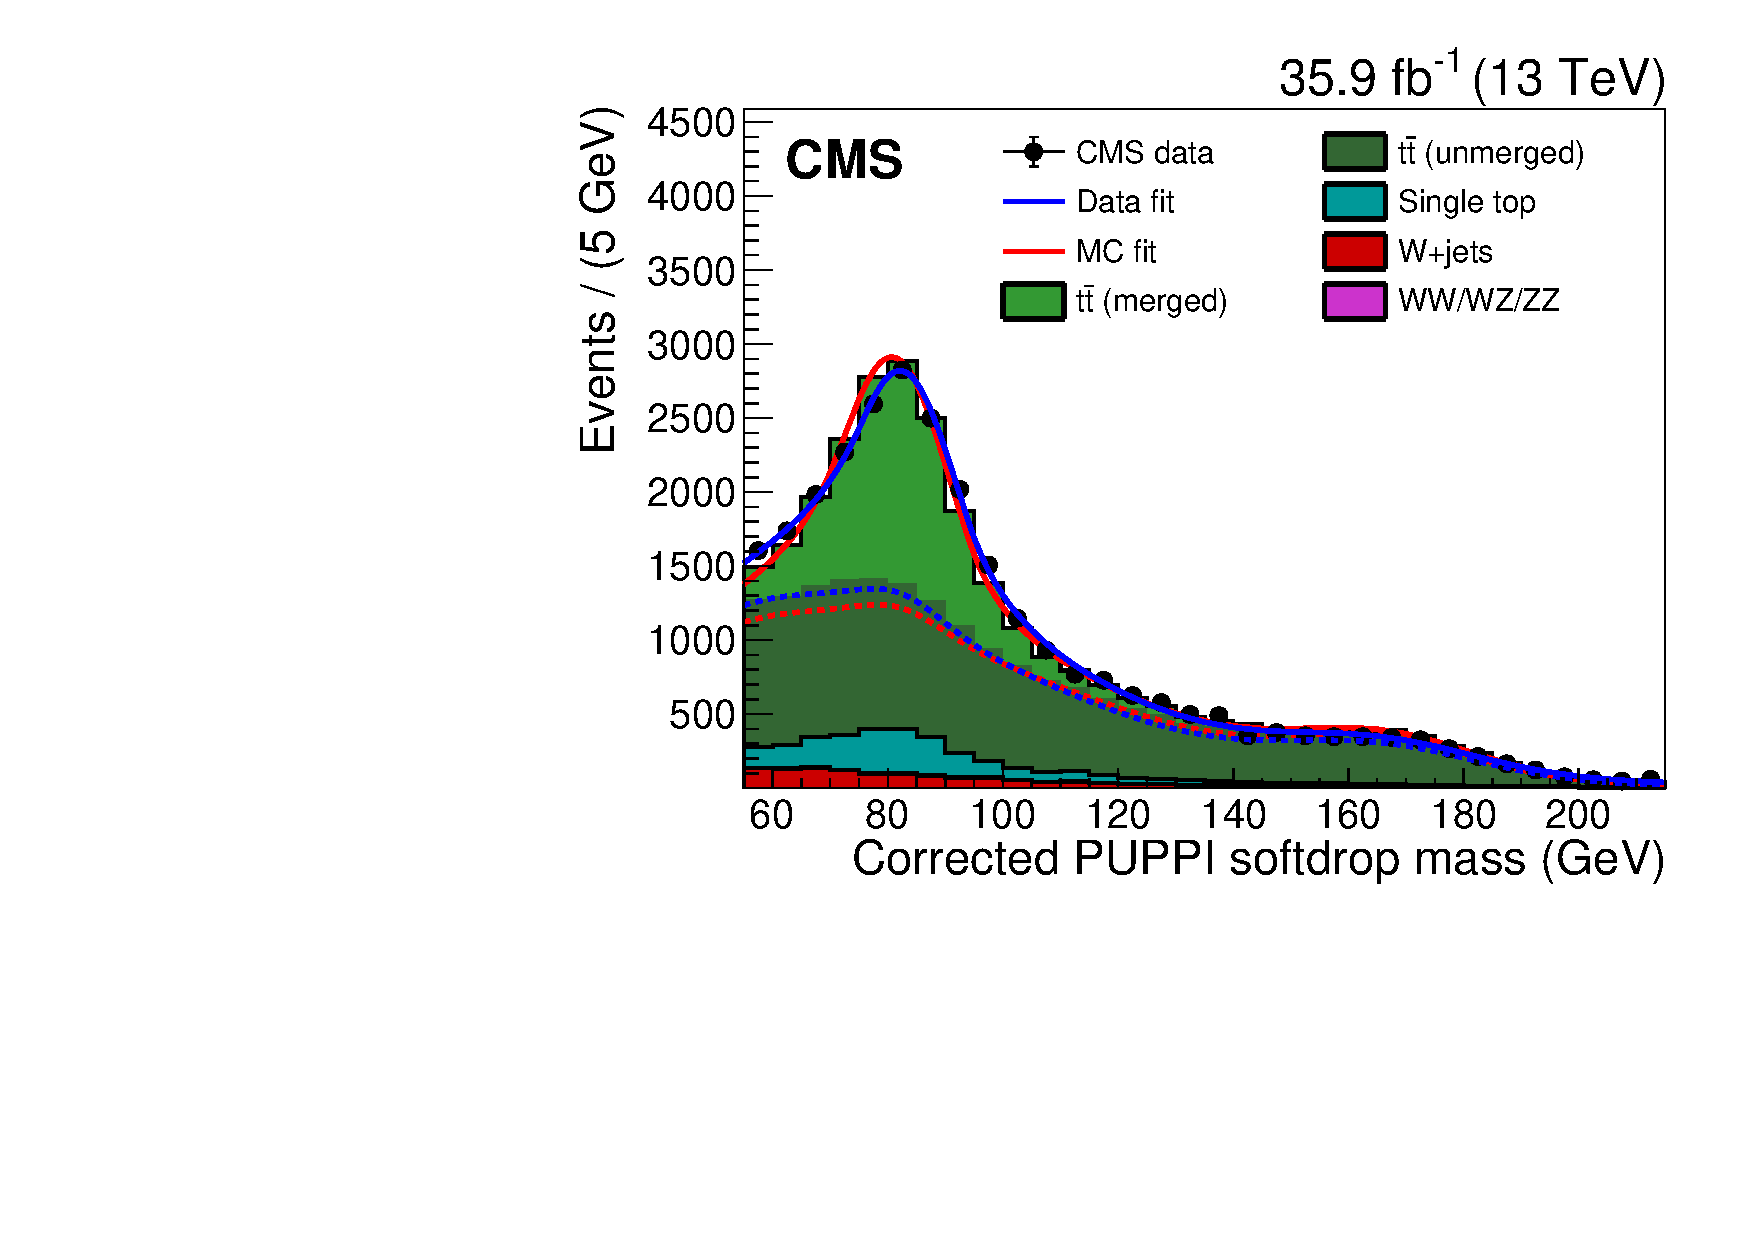
\includegraphics[width=0.49\textwidth]{figures/analysis/search3/AN-17-303/vtag/newddt_2016_fail.pdf}\\
 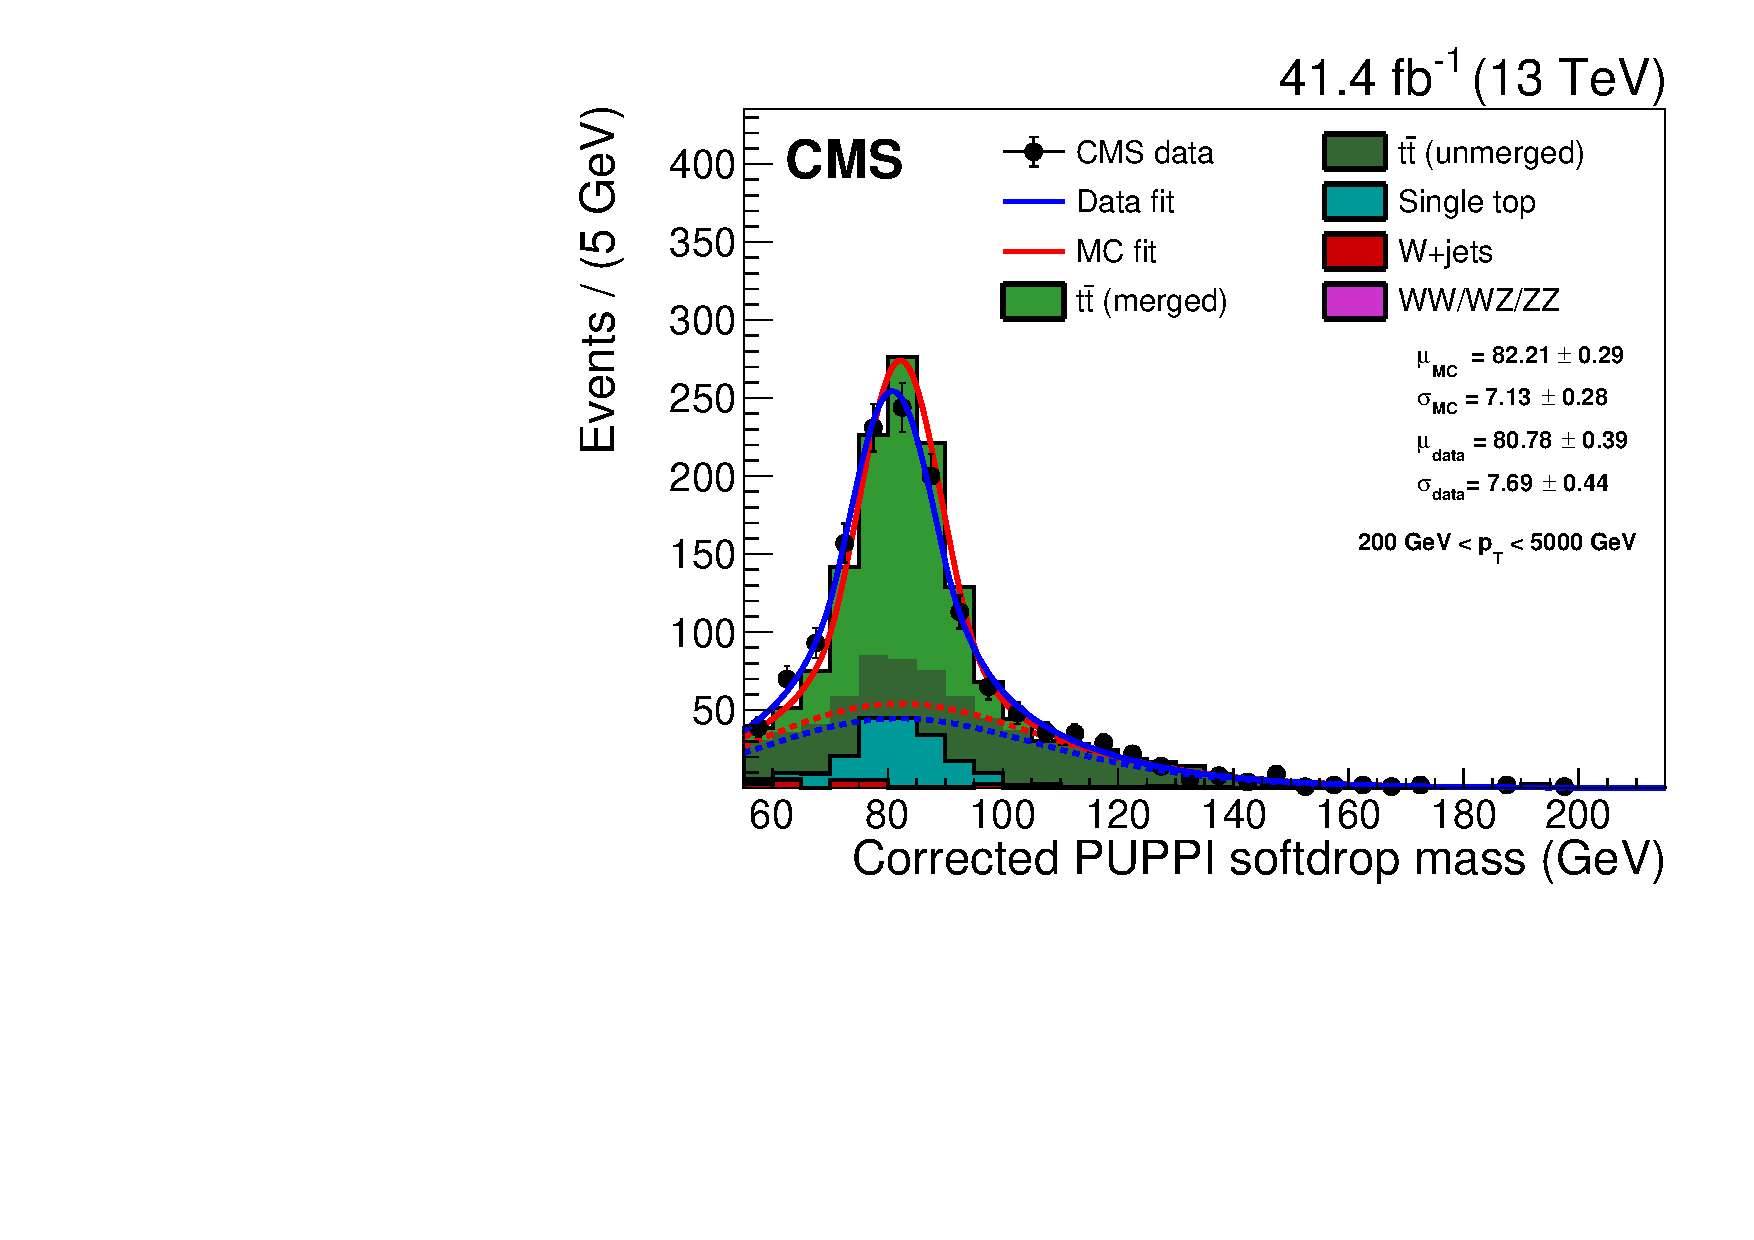
\includegraphics[width=0.49\textwidth]{figures/analysis/search3/AN-17-303/vtag/newddt_TopPtRew_2017_pass.pdf}
 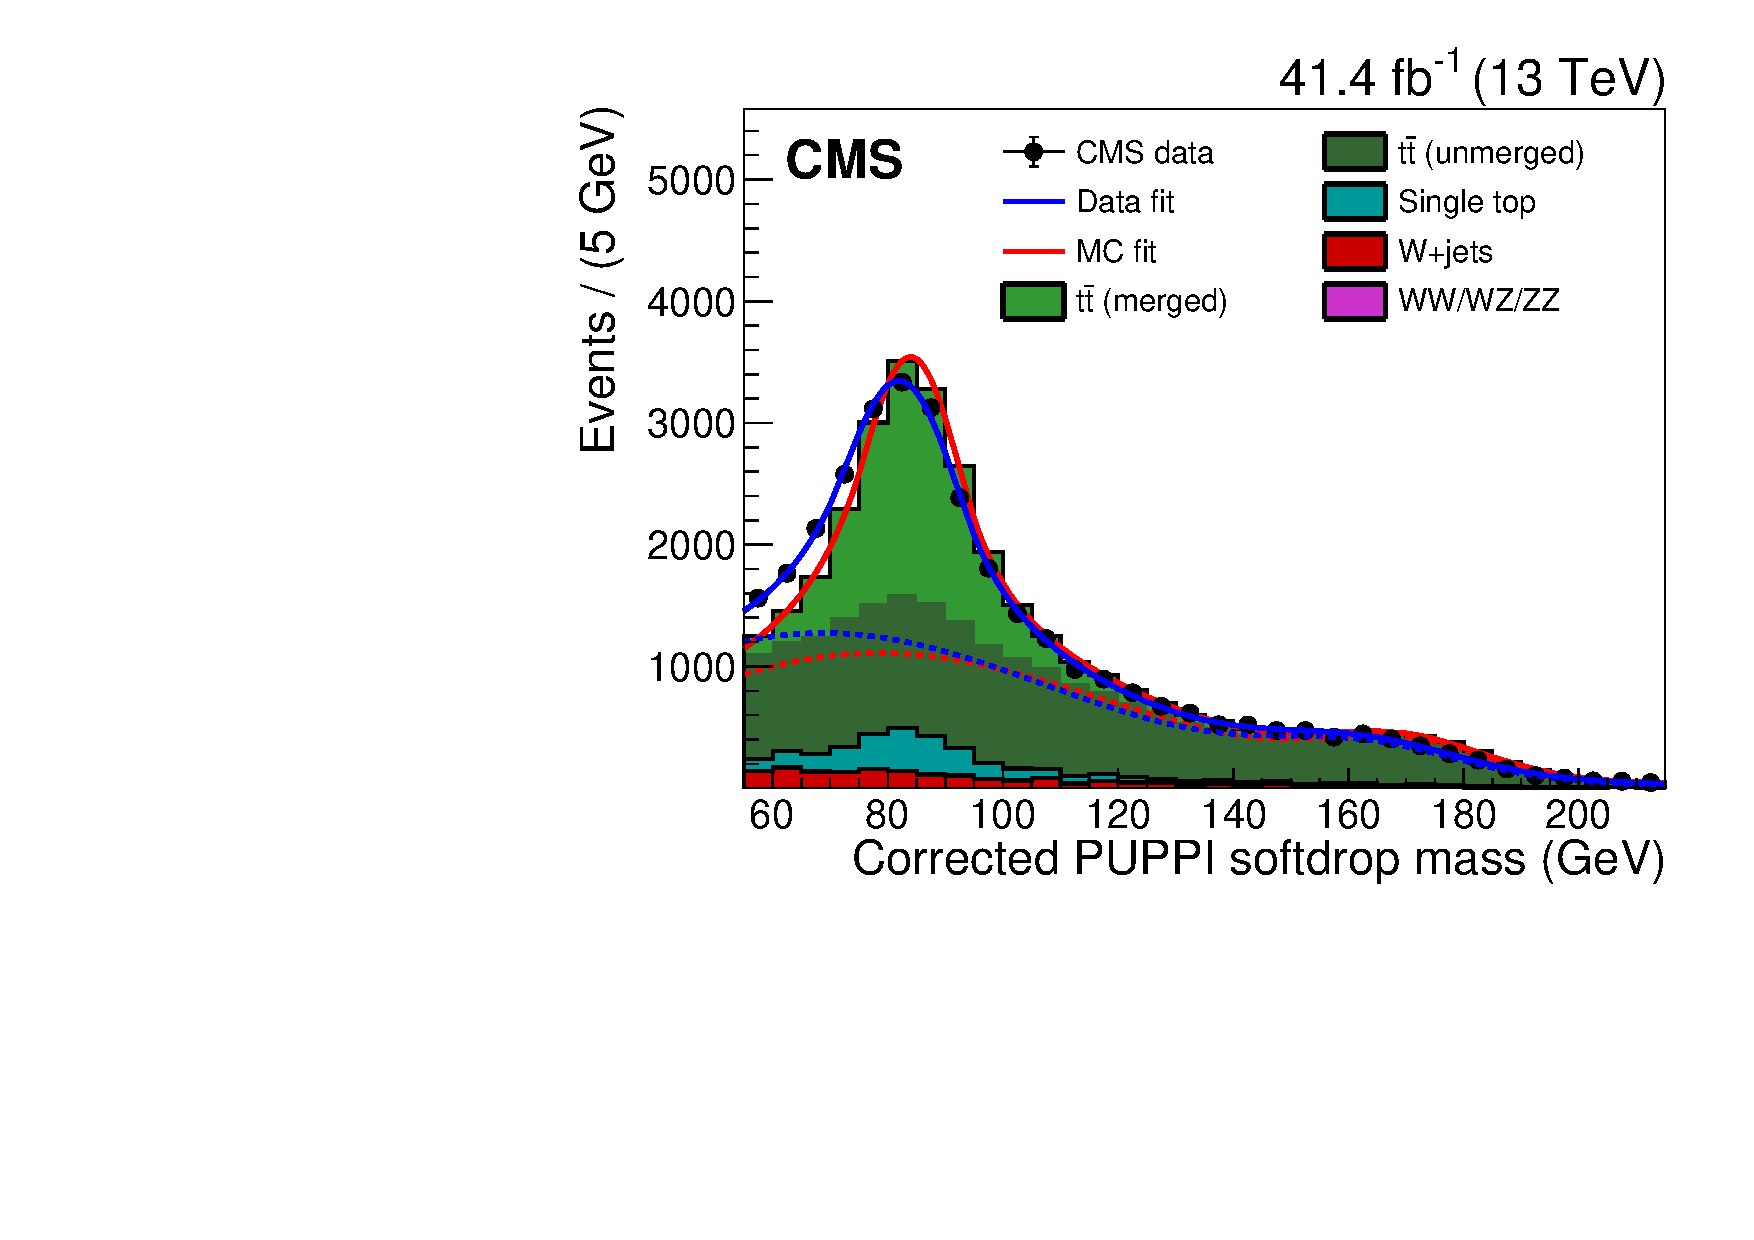
\includegraphics[width=0.49\textwidth]{figures/analysis/search3/AN-17-303/vtag/newddt_TopPtRew_2017_fail.pdf}
 \end{tabular}
 \caption{PUPPI softdrop jet mass distribution for events that pass (left) and fail (right) the $\ddt<0.43$ selection in the \ttbar control sample. The result of the fit to data and simulation is shown by the solid blue and solid red line, respectively. The background components of the fit are shown as dashed-dotted lines. The fit to 2016 data is shown in the upper panels and the fit to 2017 data in the lower panels.}
 \label{fig:simFit}
 \end{figure}
 \begin{table}[h!]
    \centering
     \begin{tabular}{|l|c|c|}
     \hline
      & SF $\pm \sqrt{\textrm{Stat.} \pm \textrm{Sys}_{\rm{Generator}} \pm \textrm{Sys}_{\rm{NNLO}}}$ & SF $\pm$ Total Unc. \\
    \hline
    $HPSF_{DDT}^{2017}$ &  $0.955 \pm \sqrt{0.113^2 \textrm{ (stat.)} + 0.003^2 \textrm{ (sys.)} + 0.043^2 \textrm{ (sys.)}}$  & $0.955 \pm 0.121$\\
    $HPSF_{DDT}^{2016}$ &  $0.937 \pm \sqrt{0.094^2 \textrm{ (stat.)} + 0.003^2 \textrm{ (sys.)} + 0.043^2 \textrm{ (sys.)}}$  & $0.937 \pm 0.103$\\
  \hline
    $LPSF_{DDT}^{2017}$ &  $1.003 \pm \sqrt{0.008^2 \textrm{ (stat.)} + 0.003^2 \textrm{ (sys.)} + 0.0^2 \textrm{ (sys.)}}$  & $1.003 \pm 0.008$\\
    $LPSF_{DDT}^{2016}$ &  $1.006 \pm \sqrt{0.009^2 \textrm{ (stat.)} + 0.003^2 \textrm{ (sys.)} + 0.0^2 \textrm{ (sys.)}}$  & $1.006 \pm 0.009$\\
     \hline
    $JMS^{2017}     $ &  $0.983 \pm \sqrt{0.006^2 \textrm{ (stat.)} + 0.002^2 \textrm{ (sys.)} + 0.001^2 \textrm{ (sys.)}}$ & $0.983 \pm 0.007$\\
    $JMS^{2016}     $ &  $1.014 \pm \sqrt{0.006^2 \textrm{ (stat.)} + 0.002^2 \textrm{ (sys.)} + 0.001^2 \textrm{ (sys.)}}$ & $1.014 \pm 0.007$\\
    \hline
    $JMR^{2017}     $ &  $1.080 \pm \sqrt{0.076^2 \textrm{ (stat.)} + 0.027^2 \textrm{ (sys.)} + 0.001^2 \textrm{ (sys.)}}$ & $1.080 \pm 0.081$\\
    $JMR^{2016}     $ &  $1.086 \pm \sqrt{0.086^2 \textrm{ (stat.)} + 0.027^2 \textrm{ (sys.)} + 0.001^2 \textrm{ (sys.)}}$ & $1.086 \pm 0.090$\\
    \hline
    \end{tabular}
       \caption{Final jet mass scale, jet mass resolution, and $\tau_{21}^{DDT}$ scalefactors with statistical and systematic uncertainties.}
       \label{tab:wsf_total}
    \end{table}
\clearpage
\subsection{\PT-dependence}
\label{sec:searchIII:vtagpt}
The $\tau_{21}^{DDT}$ selection criteria used for this search is restrictive to favor better signal significance, but results in small event samples of the data and simulation needed to produce the scale factors. In order to determine the dependence of the W-tagging efficiency, and the PUPPI softdrop jet-mass scale and resolution on the transverse momentum of the jets, we divide the sample into 4 different jet-\PT bins using the looser softdrop + \nsubj tagger, and compute the scale factors per bin. The systematic uncertainties are evaluated the same way as above (one due to top-\PT reweighting and one comparing different \ttbar samples). Figure~\ref{fig:searchIII:sfvspt} shows the extracted W-tagging efficiency for data (black markers) and for simulation (red markers) using a tagger based on PUPPI softdrop with a requirement of $\nsubj<0.4$, as a function of jet \PT. The inclusive efficiency measurement is marked with triangles. The lower panel shows the efficiency ratio of data over simulation, corresponding to the W-tagging scale factor. All scale factors are compatible with unity, but the uncertainty on the measurement grows as statistics decrease. The corresponding extracted scale factors are listed in Table~\ref{tab:searchIII:sfptdep}.
 \begin{figure}[h!]
 \centering
 \includegraphics[width=0.49\textwidth]{figures/vtagging/2017_sf/sd_vPt.pdf}
 \caption{The W-tagging efficiency in data (black circles) and in simulation (red circles) as a function of jet \PT. The \PT-inclusive measurement is marked with triangles. The lower panel shows the efficiency in data divided by the efficiency in simulation, corresponding to the W-tagging uncertainty. The blue bands mark the fit and systematic uncertainties.}
 \label{fig:searchIII:sfvspt}
 \end{figure}
\begin{table}[h!]
    \centering
    \begin{tabular}{|l|c|c|}
    \hline
     Bin & SF $\pm \sqrt{\textrm{Stat.} \pm \textrm{Sys}_{Generator} \pm \textrm{Sys}_{NNLO}}$ & SF $\pm$ Total Unc. \\
\hline
200 - 250 GeV  & $1.019  \pm \sqrt{ 0.064^2 + 0.005^2 + 0.022^2 }$ & $1.02 \pm 0.07$\\
250 - 300 GeV  & $1.058  \pm \sqrt{ 0.055^2 + 0.033^2 + 0.002^2 }$ & $1.06 \pm 0.06$\\
300 - 350 GeV  & $0.998  \pm \sqrt{ 0.087^2 + 0.035^2 + 0.007^2 }$ & $1.00 \pm 0.09$\\
350 - 600 GeV  & $0.898  \pm \sqrt{ 0.097^2 + 0.089^2 + 0.007^2 }$ & $0.90 \pm 0.13$\\
\hline
$\geq$ 200 GeV & $0.974  \pm \sqrt{ 0.029^2 + 0.055^2 + 0.015^2 }$ & $0.97 \pm 0.06$\\
    \hline
    \end{tabular}
    \caption{The data to simulation scale factors in bins of jet \PT for a tagger based on PUPPI softdrop with a requirement of $\nsubj<0.4$. All scalefactors are compatible with unity.}
    \label{tab:searchIII:sfptdep}
 \end{table}
With the observation of this clear trend of an uncertainty increase as a function of \PT, we evaluate a \PT-dependent W-tagging scale factor uncertainty in the following way: using signal Monte Carlo generated with two different shower generators, \PYTHIA{8} and \HERWIG{++}, we compute the difference in tagging efficiency between the two samples at low-\PT, where we have a real measurement in data, and compare that to the difference in tagging efficiency between the two at high-\PT. In other words, we take a double ratio 
\begin{equation}
  \sigma_{p_{T,\textrm{Bin}=i}}=\frac{ (\frac{\epsilon_{\PYTHIA}}{\epsilon_{\HERWIG}})_{p_{T,\textrm{Bin}=i}}} {(\frac{\epsilon_{\PYTHIA}}{\epsilon_{\HERWIG}})_{300 \GeV}},
  \end{equation}
where $\sigma_{p_{T,\textrm{Bin}=i}}$ is the uncertainty on the scale factor on \PT bin $i$. In contrast with what was found for the \nsubj-based tagger in Section~\ref{sec:searchI:wtagsystematic}, where this uncertainty grew logarithmically with \PT, we find that the corresponding double ratio stabilizes around 1 \TeV in the high-purity category when using \ddt, and that it is better described by a sigmoid function. The uncertainty for the low-purity category is still well described by a logarithmic function. The resulting parametrization of $\sigma_{p_{T}}$ using a sigmoid fit, is shown in Figure~\ref{fig:searchIII:tau21ptdep}.
 \begin{figure}[h!]
 \centering
 \includegraphics[width=0.49\textwidth]{figures/vtagging/2017_sf/ptdep.pdf}
 \caption{The parametrized uncertainty on the W-tagging efficiency scale factor as a function of the jet \PT.}
 \label{fig:searchIII:tau21ptdep}
 \end{figure}
In my personal opinion, this way of defining an uncertainty is rather random and ad hoc. We already know there is a large difference in the modeling of substructure variables between generators, and there is no good reason to believe the difference between \PYTHIA{8} and \HERWIG{++} provides a reasonable description of the magnitude of the uncertainty. In an analysis using two jets this is a very large and overly conservative systematic uncertainty that is impossible to constrain from data. I would rather prefer to use the measured scale factor uncertainties in data and extrapolate these, but the above method was used in previous searches and is therefore the method of choice for the Jet Physics Object Group at CMS. I will therefore continue using these uncertainties for the presented analysis, but will attempt to change this for future searches.
In addition to measuring the dependence of the tagging efficiency on jet \PT, we  also extract the change in softdrop jet-mass scale and resolution as a function of \PT. We find that the jet-mass scale in data divided by MC ranges between 0.5 and 2.5\% for the \PT bins considered, and the jet-mass resolution varies between 4 and 10\%, the latter measurement not being statistically significant as the uncertainties are large, around 10\%. For this analysis, we therefore use a fixed uncertainty of 2 and 10\% for the softdrop jet-mass scale and resolution, respectively, to cover any broadening or shift at high \PT not described by the simulation.
   
\clearpage    
\section{The multidimensional fit}
\label{sec:searchIII:fit3d}
The three-dimensional fit method is based on the assumption that the signal peaks in three dimensions: the dijet invariant mass ($\MVV$), the groomed jet mass of the first jet ($\MJO)$, and the groomed jet mass of the second jet ($\MJT$), in order to extract a possible signal from the three-dimensional $\MJO$-$\MJT$-$\MVV$ (x,y,z) plane.\newline
\begin{figure}[h!]
\centering
\includegraphics[width=0.99\textwidth]{figures/analysis/search3/misc/3Dfit.png}
\caption{An illustration of the shape of the signal and the relative background contributions in the three dimensions $\MJO$(x), $\MJT$(y) and $\MVV$(z). }
\label{fig:searchIII:3Dfit}
\end{figure}
\noindent In order to obtain a complete three-dimensional model, four different types of probability density functions (PDF's) need to be derived:
\begin{itemize}
   \itemsep0em
  \item \textbf{signal:} a PDF resonant in $\MJO$, $\MJT$ and $\MVV$,
  \item \textbf{non-resonant background:} PDF for the dominant QCD multijet background. Non-resonant in $\MJO$, $\MJT$ and $\MVV$,
  \item \textbf{resonant background:} PDF describing of W+jets and Z+jets. Resonant in $\MJO$ and $\MJT$, but smoothly falling in $\MVV$, and
  \item \textbf{alternative shapes:} five additional shape uncertainties for the non-resonant background.
\end{itemize}
These are illustrated in Figure~\ref{fig:searchIII:3Dfit} and will be described in detail in the following.
\clearpage

\subsection{Modeling of the signal}
The signal shape in three dimensions is defined as the product of the resonance mass shape and the jet mass shapes:
\begin{equation}
	\footnotesize
	P_{sig}(\MVV,\MJO,\MJT|\theta(M_X) ) = P_{VV}(\MVV|\theta_1(M_X)) \times P_{j1}(\MJO|\theta_2(M_X))\\ \times P_{j2}(\MJT|\theta_2(M_X)).
\end{equation} 
The shapes for \MVV, \MJO and \MJT all depend on the hypothesized mass of the new particle ($M_X$) and a set of parameters $\theta=(\theta_1, \theta_2)$ that in principle depend on $M_X$. The modeling of \MJ is done separately for the high-purity and the low-purity category, while the modeling of \MVV is done with no selection on \ddt applied (\MVV was found to be decorrelated from \ddt for signal jets).\par
The signal is parametrized by fitting the resonance mass and jet-mass line shapes for each resonance mass value, extracting the fitted parameters and then interpolating these as a function of the resonance-mass hypothesis. For the resonance mass \MVV, the sum of a crystal-ball function and a Gaussian shape is used for each mass point, following the shapes used in Search II. Figure~\ref{fig:MVVShapeParam} shows the derived parameters and interpolation as a function of resonance mass, and the final \MVV shapes as extracted from the parametrization are shown in Figure~\ref{fig:MVVfromjson}.
\begin{figure}[h!]
\centering
\resizebox{0.327\textwidth}{!}{\includegraphics*{figures/analysis/search3/AN-17-303/signalFits/Signal_mVV_MEAN.pdf}}
\resizebox{0.327\textwidth}{!}{\includegraphics*{figures/analysis/search3/AN-17-303/signalFits/Signal_mVV_SIGMA.pdf}}
\resizebox{0.327\textwidth}{!}{\includegraphics*{figures/analysis/search3/AN-17-303/signalFits/Signal_mVV_ALPHA1.pdf}}\\
\resizebox{0.327\textwidth}{!}{\includegraphics*{figures/analysis/search3/AN-17-303/signalFits/Signal_mVV_ALPHA2.pdf}}
\resizebox{0.327\textwidth}{!}{\includegraphics*{figures/analysis/search3/AN-17-303/signalFits/Signal_mVV_N1.pdf}}
\resizebox{0.327\textwidth}{!}{\includegraphics*{figures/analysis/search3/AN-17-303/signalFits/Signal_mVV_N2.pdf}}
\caption{The interpolated fit parameters of a crystal-ball fit to the dijet invariant mass as a function of $M_X$. The small variations for ALPHA2 have been shown to have no effect on the overall modeling.}
\label{fig:MVVShapeParam}
\end{figure}
\begin{figure}[h!]
\centering
\resizebox{0.6\textwidth}{!}{\includegraphics*{figures/analysis/search3/AN-17-303/signalFits/signalShapes_mVV_All.pdf}}
\caption{Final $\MVV$ signal shapes extracted from the parametrization. Here for a $\BulkG$ decaying to WW (blue), ZZ (red), and for a $\Wpr$ decaying to WZ (green).}
\label{fig:MVVfromjson}
\end{figure}
The same procedure is used to model the jet mass; the \MJ spectrum for each resonance mass hypothesis is fitted using a double Crystal-ball function, and the fitted parameters are extracted and interpolated as a function of the resonance mass. This is done separately for $\MJO$ and $\MJT$. The fitted parameters and interpolations are shown in Figure~\ref{fig:MJet1ShapeParam} for \MJO, and the corresponding distributions for \MJT can be found in Appendix~\ref{app:search3:sigfits}.
\begin{figure}[h!]
\centering
\resizebox{0.327\textwidth}{!}{\includegraphics*{figures/analysis/search3/AN-17-303/signalFits_2016/Signal_mjetl1_mean.pdf}}
\resizebox{0.327\textwidth}{!}{\includegraphics*{figures/analysis/search3/AN-17-303/signalFits_2016/Signal_mjetl1_sigma.pdf}}
\resizebox{0.327\textwidth}{!}{\includegraphics*{figures/analysis/search3/AN-17-303/signalFits_2016/Signal_mjetl1_alpha.pdf}}\\
\resizebox{0.327\textwidth}{!}{\includegraphics*{figures/analysis/search3/AN-17-303/signalFits_2016/Signal_mjetl1_alpha2.pdf}}
\resizebox{0.327\textwidth}{!}{\includegraphics*{figures/analysis/search3/AN-17-303/signalFits_2016/Signal_mjetl1_n.pdf}}
\resizebox{0.327\textwidth}{!}{\includegraphics*{figures/analysis/search3/AN-17-303/signalFits_2016/Signal_mjetl1_n2.pdf}}
\caption{The interpolated double Crystal-ball parameters for the softdrop jet mass as a function of $M_X$. To improve the stability of the fit some parameters are set constant.}
\label{fig:MJet1ShapeParam}
\end{figure}
The final \MJO shapes, as extracted from the parametrization are shown in Figures~\ref{fig:MJfromjson}.
\begin{figure}[h!]
\centering
\resizebox{0.6\textwidth}{!}{\includegraphics*{figures/analysis/search3/AN-17-303/signalFits/signalShapes_mJ_All.pdf}}
\caption{Final $\MJ$ signal shapes extracted from the parametrization for a $\BulkG$ decaying to ZZ (red), a $\BulkG$ decaying to WW (blue), and for a $\Wpr$ decaying to WZ (green).}
\label{fig:MJfromjson}
\end{figure}
Finally, the signal yield is parametrized as a function of the resonance mass. For each mass point $M_X$ and each purity category, the signal yield per picobarn of cross section is calculated as the integral of the resulting Monte Carlo histogram after all analysis selections have been applied.
The yields are then interpolated as a function of $M_X$. The signal efficiency as a function of resonance mass is shown in Figure~\ref{fig:SignalYields}.
\begin{figure}[h!]
\centering
\resizebox{0.6\textwidth}{!}{\includegraphics*{figures/analysis/search3/AN-17-303/signalFits_2016/signalEff.pdf}}
\caption{Signal efficiency as a function of resonance mass.}
\label{fig:SignalYields}
\end{figure}
\clearpage


\subsection{Modeling of the non-resonant background}
\label{sec:nonresbkgd}

In order to model the QCD multijets background in the three-dimensional \MVV-\MJO-\MJT plane, we use the following conditional product:
\begin{equation}
	\footnotesize
	P(\MVV,\MJO,\MJT) = P_{VV}(\MVV|\theta_1) \times P_{cond,1}(\MJO|\MVV,\theta_2) \times P_{cond,2}(\MJT|\MVV,\theta_2).
\end{equation} 
This probability density requires a computation of the conditional two-dimensional shapes of $\MJO$ or $\MJT$, given $\MVV$, as well as a one dimensional shape of the $\MVV$ distribution. The reason for requiring a conditional jet-mass shape, is due to the high correlation between the jet mass and the dijet invariant mass for quark and gluon jets. The modeling is done separately for the high-purity and the low-purity category.\par
The following fit ranges are used for the three axes: the jet masses \MJO and \MJT are fitted from 55 to 215 GeV using 2 GeV bins, and the dijet invariant mass $\MVV$ is fitted from 1126 to 5500 GeV. The lower $\MVV$ bound is chosen to avoid complications in the fitting procedure due to trigger turn-on effects, while the upper $\MVV$ bound is chosen by considering the highest dijet invariant mass event found in data. For $\MVV$, the "dijet binning", corresponding to the dijet mass resolution, is used. In units of \GeV, the binning is as follows:\newline


\noindent Dijet binning = 1126, 1181, 1246, 1313, 1383, 1455, 1530, 1607, 1687, 1770, 1856, 1945, \\
2037, 2132, 2231, 2332, 2438, 2546, 2659, 2775, 2895, 3019, 3147, 3279, 3416, 3558, 3704, \\
3854, 4010, 4171, 4337, 4509, 4686, 4869, 5058, 5253, 5500.\newline


\noindent The background model is built starting from simulation using a "forward-folding" approach. To build the one-dimensional template for the dijet invariant mass, $P_{VV}(\MVV|\theta_1)$, a 1D Gaussian kernel is built starting from generator level quantities where, for each MC event, a Gaussian contributes to the total one-dimensional probability density function. To build the two-dimensional conditional templates, $P_{cond,1}(\MJO|\MVV,\theta_2) $ and $ P_{cond,2}(\MJT|\MVV,\theta_2)$, a two-dimensional Gaussian kernel is created for each MC event, where each 2D kernel contributes to the total conditional PDF.  \par
In order to define the Gaussian kernel, the dijet invariant mass scale and resolution, and the softdrop jet-mass scale and resolution, must be derived. 
This is done by comparing the generated jet-mass $M(\mathrm{gen})$ to the reconstructed jet-mass $M(\mathrm{reco})$. The $\MJ$ and $\MVV$ scale and resolution are extracted from a Gaussian fit to either $\MJ(\mathrm{reco})/\MJ(\mathrm{gen})$ or $\MVV(\mathrm{reco})/\MVV(\mathrm{gen})$, in bins of generator-level jet \PT. Figure~\ref{fig:resoFits} shows the fit to $M_{jet}(\mathrm{reco})/M_{jet}(\mathrm{gen})$ (left) and $M_{jj}(\mathrm{reco})/M_{jj}(\mathrm{gen})$ (right) for an arbitrary \PT bin. The mean of the Gaussian yields the jet-mass scale and the width yields the jet-mass resolution, for a given bin in generator-level jet \PT.
\begin{figure}[h!]
\centering
\resizebox{0.4\textwidth}{!}{\includegraphics*{figures/analysis/search3/AN-17-303/detRes/detectorResolution/debug_fit_mjres_8.png}}
\resizebox{0.4\textwidth}{!}{\includegraphics*{figures/analysis/search3/AN-17-303/detRes/detectorResolution/debug_fit_mvvres_8.png}}\\
\caption{Left: fit to $\MJ(\mathrm{reco})/\MJ(\mathrm{gen})$. Right: fit to $\MVV(\mathrm{reco})/\MVV(\mathrm{gen})$. 
The mass resolution is taken as the width of the fitted Gaussian, while the Gaussian mean yields the mass scale.}
\label{fig:resoFits}
\end{figure}
The $\MJ$ and $\MVV$ jet mass scale and resolution as a function of generator jet $\PT$ is shown in Figure~\ref{fig:ScaleResolution}, and the total projection of these resolution functions are shown in Figure~\ref{fig:ResolutionProfiles}.
\begin{figure}[h!]
\centering
\resizebox{0.4\textwidth}{!}{\includegraphics*{figures/analysis/search3/AN-17-303/detRes/detectorresolution_resxHisto.png}}
\resizebox{0.4\textwidth}{!}{\includegraphics*{figures/analysis/search3/AN-17-303/detRes/detectorresolution_resyHisto.png}}\\
\resizebox{0.4\textwidth}{!}{\includegraphics*{figures/analysis/search3/AN-17-303/detRes/detectorresolution_scalexHisto.png}}
\resizebox{0.4\textwidth}{!}{\includegraphics*{figures/analysis/search3/AN-17-303/detRes/detectorresolution_scaleyHisto.png}}
\caption{The $\MVV$ resolution (top left) and scale (bottom left), and the $\MJ$ resolution (top right) and scale (bottom right) as a function of generator-level jet $\PT$.}
\label{fig:ScaleResolution}
\end{figure}
\begin{figure}[h!]
\centering
\resizebox{0.4\textwidth}{!}{\includegraphics*{figures/analysis/search3/AN-17-303/detRes/detectorresolution_mvv.png}}
\resizebox{0.4\textwidth}{!}{\includegraphics*{figures/analysis/search3/AN-17-303/detRes/detectorresolution_mjet.png}}\\
\caption{Projections of the resolution functions for all generator-level jet $\PT$ bins for $\MVV$ (left) and $\MJ$ (right).}
\label{fig:ResolutionProfiles}
\end{figure}
The jet-mass and the dijet invariant mass scale and resolution are then used to populate the conditional 2D histogram as follows. Each generated event is smeared with a 2D Gaussian kernel of the form
\begin{equation}
k(\MJ,\MVV) =\frac{w_i}{\sqrt{2\pi}r_{\MVV,i}\cdot r_{\MJ,i}} \exp \left (-\frac{1}{2} \left ( \frac{\MVV-s_{\MVV,i}}{r_{\MVV,i}} \right)^2 -\frac{1}{2} \left ( \frac{\MJ-s_{\MJ,i}}{r_{\MJ,i}} \right)^2 \right ),   
\end{equation}
where $s_{i}, r_{i}$ are the scale and the resolution derived in the previous step and $w_i$ is the event weight product due to effects such as PU-reweighting and cross-sections. The resulting kernel values are then filled into a 2D histogram. This procedure is performed separately for \MJO and \MJT. To build the one-dimensional template for the dijet invariant mass, the same procedure as above is used with the exception that the smearing is done with a one-dimensional Gaussian kernel only depending on $\MVV$. The three templates are then added together to form a three-dimensional PDF, and this PDF is fitted to QCD MC in order to remove any residual bias. The result is a smooth shape, covering the entire search range, that can be used in place of the prediction from simulation.\par
As the high-purity category is limited by statistics, we instead build this template starting from the low-purity templates. This is done by fitting the low-purity 3D template, obtained using the method described above, to QCD MC in the high-purity category. Figure~\ref{fig:searchIII:3Dkernels} shows the final templates (solid lines) together with the QCD MC (data points) derived from the 2017 MC in the low-purity (top) and high-purity (bottom) category. Good agreement between simulation and templates in all three dimensions is observed, within statistical uncertainties. The corresponding distributions for 2016 MC can be found in Appendix~\ref{app:search3:2016kernels}.\par
\begin{figure}[h!]
\centering
\resizebox{0.328\textwidth}{!}{\includegraphics*{figures/analysis/search3/AN-17-303/backgroundFits/3Dkernels_HPLP_pythia_2017/cx.png}}
\resizebox{0.328\textwidth}{!}{\includegraphics*{figures/analysis/search3/AN-17-303/backgroundFits/3Dkernels_HPLP_pythia_2017/cy.png}}
\resizebox{0.328\textwidth}{!}{\includegraphics*{figures/analysis/search3/AN-17-303/backgroundFits/3Dkernels_HPLP_pythia_2017/cz.png}}\\
\resizebox{0.328\textwidth}{!}{\includegraphics*{figures/analysis/search3/AN-17-303/backgroundFits/3Dkernels_HPHP_pythia_2017/cx.png}}
\resizebox{0.328\textwidth}{!}{\includegraphics*{figures/analysis/search3/AN-17-303/backgroundFits/3Dkernels_HPHP_pythia_2017/cy.png}}
\resizebox{0.328\textwidth}{!}{\includegraphics*{figures/analysis/search3/AN-17-303/backgroundFits/3Dkernels_HPHP_pythia_2017/cz.png}}
\caption{Comparison between QCD MC simulation (markers) and kernels derived from generator-level quantities (lines) for the HP (top) and LP (bottom) categories using 2017 MC. The kernels are shown for \MJO (left), \MJT (middle) and \MVV (right).}
\label{fig:searchIII:3Dkernels}
\end{figure}
In order to validate the kernel-transfer method, we check that we can fit a higher-statistics high-purity region by loosening the $\tau_{21}^{DDT}$ cut to 0.49. This results in 12 times more background events, and should uncover whether any degeneracy is present in the fits themselves and whether the low-purity kernel indeed is capable of modeling the high-purity region. The resulting kernel-versus-MC spectra are shown in Figure~\ref{fig:searchIII:looseDDT_closure}. Good closure is observed in all three dimensions, demonstrating that the LP kernels adapt well to the HP MC data points even when statistics are sufficient, and we therefore consider the method to be sound.
\begin{figure}[h!]
\centering
\resizebox{0.328\textwidth}{!}{\includegraphics*{figures/analysis/search3/AN-17-303/backgroundFits/looseDDT_HPHP/cx.png}}
\resizebox{0.328\textwidth}{!}{\includegraphics*{figures/analysis/search3/AN-17-303/backgroundFits/looseDDT_HPHP/cy.png}}
\resizebox{0.328\textwidth}{!}{\includegraphics*{figures/analysis/search3/AN-17-303/backgroundFits/looseDDT_HPHP/cz.png}}
\caption{Comparison between QCD MC simulation (markers) and kernels derived from generator-level quantities (lines) in the HP category, using a looser cut on $\tau_{21}^{DDT}$.}
\label{fig:searchIII:looseDDT_closure}
\end{figure}
\clearpage

\subsection{Modeling of the resonant background}
\label{sec:resbkgd}
In addition to the QCD multijet background, there are a few sub-dominant processes which contain one real vector boson and at least one QCD-jet that must be accounted for. These are W+jets, Z+jets and events from \ttbar processes. These events are resonant in \MJO and \MJT and must therefore be treated differently than the non-resonant QCD background. Figure \ref{fig:stack_res_bkg} shows the projections on \MJO (left), \MJT (middle) and \MVV (right) for the resonant backgrounds under consideration.
\begin{figure}[h!]
 \includegraphics[width=0.329\textwidth]{figures/analysis/search3/AN-17-303/resonantBkg/CP_background_px_xrange55-215_yrange55-215zrange1126-5000_HPLP.pdf}
 \includegraphics[width=0.329\textwidth]{figures/analysis/search3/AN-17-303/resonantBkg/CP_background_py_xrange55-215_yrange55-215zrange1126-5000_HPLP.pdf}
 \includegraphics[width=0.329\textwidth]{figures/analysis/search3/AN-17-303/resonantBkg/CP_background_pz_xrange55-215_yrange55-215zrange1126-5000_HPLP.pdf}
\caption{Projections of the sub-dominant backgrounds on the jet mass axes \MJO (left) and \MJT (middle), as well as on the dijet invariant mass \MVV (right). Here in the low-purity category.}
\label{fig:stack_res_bkg}
\end{figure}
As the jets are randomly sorted, each jet mass distribution contains two contributions: a resonant part consisting of real vector-boson jets, peaking around the W or Z boson mass; and a non-resonant part composed of jets originating from a quark or a gluon, similar to the QCD-multijets background. These two contributions are modeled separately since we know that the non-resonant part of the jet mass spectrum is correlated with the dijet invariant mass (as was the case for QCD), while the resonant part is not (as was the case for the signal PDF). We additionally want to encode the information that these backgrounds in reality have only one real vector boson and so only peak in one jet-mass dimension, by requiring the PDFs to consist of a resonant part on one axis, and a non-resonant part on the other axis. A three-dimensional PDF for the resonant backgrounds is built as a product of three one-dimensional PDFs as follows:
\begin{align}
	\label{eq:searchIII:vjetpdf}
	P_{res} \left(\MJO, \MJT, \MVV \right) &= P_{VV} \left( \MVV \right) \times  P_{jet1} \left( \MJO, \MJT \right) \times P_{jet2} \left( \MJT, \MJO \right),
\end{align}
where
\begin{align}
P_{jet1} \left( \MJO, \MJT \right) &= f \times R(\MJT) \times P_{res,1} ( \MJO ) + (1-f) P_{non-res,1} (\MJO )\textrm{ and } \\
P_{jet2} \left( \MJT, \MJO \right) &= (1-f) \times R(\MJO) \times P_{res,2} ( \MJT ) + f P_{non-res,2} (\MJT ).
\end{align}
Here, $R(\MJ)$ parametrizes the correlation between \MJO and \MJT and $f$ is a fit parameter that is used to adjust the fraction of real vector boson jets in
\MJO compared to \MJT. Its value can vary by 10\% around $f=0.5$, the expected median when using a random jet sorting. $P_{res,1}$ and $P_{res,1}$ are PDFs describing the resonant part of the jet mass spectrum, while $P_{non-res,1}$ and $P_{non-res,2}$ describe the non-resonant part. The functional form of these will be described below. \newline
As the contribution of background from \ttbar is much smaller than the one coming from V+jets (less than 2\%), this background is modeled together with the W+jets contribution. Therefore only two PDFs are built for the resonant background: one for the W+jets and \ttbar processes, and one for the Z+jets process.\newline
The available MC statistics in the high-purity category are very low and therefore the parametrization of the resonant background is done for the low-purity category only, and the resulting shapes are then used for both purity categories. The uncertainties for the different purity categories are, however, included as separate nuisance parameters in the fit.\par
The non-resonant \MVV PDF is constructed using the same kernel approach as is used to model the QCD multijet background with one minor difference: due to the low statistics in the high-\MVV tail, an additional smoothing of the jet mass tail using a leveled exponential of the form
\begin{equation}
\frac{\text{d} N}{\text{d} m_{jj}} = \frac{P_0 (1-m_{jj}/s)^{P_1}}{(m_{jj}/s)^{P_2}}
\end{equation}
is performed. Here, $s$ is the center-of-mass energy. The function is fitted to the spectrum starting from a dijet mass of 1.1 (2.1)~TeV for the high-purity (low-purity) category. Two uncertainties on the shape are added in order to accommodate possible MC mis-modeling due to higher order QCD and electroweak corrections: one proportional to \MVV and one proportional to 1/\MVV. The resulting \MVV kernels (solid lines) for the W+jets background are shown in Figure \ref{fig:Vjets_mvv} and are compared to MC simulation (markers). The blue line corresponds to the nominal shape, while the red and green lines correspond to the uncertainties proportional to \MVV and 1/\MVV, respectively. The corresponding distributions for the Z+jets background are shown in Appendix~\ref{app:search3:resbkg}.\par
\begin{figure}[h]
\centering
\resizebox{0.49\textwidth}{!}{\includegraphics*{figures/analysis/search3/AN-17-303/resonantBkg/debug_mVV_kernels_WJets_HPHP.png}}
\resizebox{0.49\textwidth}{!}{\includegraphics*{figures/analysis/search3/AN-17-303/resonantBkg/debug_mVV_kernels_WJets_HPLP.png}}\\
% \resizebox{0.49\textwidth}{!}{\includegraphics*{figures/analysis/search3/AN-17-303/resonantBkg/debug_mVV_kernels_ZJets_HPHP.pdf}}
% \resizebox{0.49\textwidth}{!}{\includegraphics*{figures/analysis/search3/AN-17-303/resonantBkg/debug_mVV_kernels_ZJets_HPLP.pdf}}
\caption{One-dimensional \MVV kernels (solid line) compared to MC (markers) for the W+jets background in the HP (left) and LP (right) categories. The blue line corresponds to the nominal shape, while the red and green lines correspond to uncertainties proportional to \MVV and 1/\MVV, respectively.}
\label{fig:Vjets_mvv}
\end{figure}
As mentioned above, the modeling of the \MJ spectrum is split into two different PDFs: one describing the resonant and one describing the non-resonant part. We distinguish between the two by requiring the resonant contribution to consist of jets matched to a generated boson within a cone of $\Delta R = 0.8$. A double-sided crystal-ball function is then fitted to the resonant spectrum for W+jets and Z+jets separately. The uncertainty on the mean and width of the \MJ distribution are fully correlated between signal and the resonant background, as these uncertainties affect all jets generated by a real vector bosons in the same way. This effectively gives us a way of constraining these parameters directly from data. The parametrization of the resonant part of the jet mass spectrum for \MJO is shown in Figure \ref{fig:Vjets_fits} for W+jets and \ttbar (left), and Z+jets (right). The small enhancement around 170 \GeV is caused by fully merged top jets, but is so small ($<2\%$ in the low-purity and $<0.5\%$ in the high-purity category) that we do not take it into account in the final PDF.
\begin{figure}[h!]
\centering
\resizebox{0.45\textwidth}{!}{\includegraphics*{figures/analysis/search3/AN-17-303/resonantBkg/debugJl1_Wjets_TTbar_Res.png}}
\resizebox{0.45\textwidth}{!}{\includegraphics*{figures/analysis/search3/AN-17-303/resonantBkg/debugJl1_Zjets_Res.png}}
\caption{Fit to the resonant part of the V+jets and \ttbar spectrum for W+jets and \ttbar (left) and Z+jets (right).}
\label{fig:Vjets_fits}
\end{figure}
The non-resonant part of the V+jets background is modeled using a simple Gaussian fit to the spectrum of jets not matched to real vector bosons, as shown in Figure \ref{fig:Vjets_fits_nonRes}.
\begin{figure}[h!]
\centering
\resizebox{0.49\textwidth}{!}{\includegraphics*{figures/analysis/search3/AN-17-303/resonantBkg/debugJl1_Wjets_TTbar_nonRes.png}}
\resizebox{0.49\textwidth}{!}{\includegraphics*{figures/analysis/search3/AN-17-303/resonantBkg/debugJl1_Zjets_nonRes.png}}
\caption{Fit to the non-resonant part of the V+jets and \ttbar spectrum for W+jets and \ttbar (left) and Z+jets (right).}
\label{fig:Vjets_fits_nonRes}
\end{figure}
For the resonant modeling, correlations between the jet mass \MJ and dijet invariant mass \MVV have been found small enough to be neglected; the jet mass spectrum does not, within statistical uncertainties, depend on the jet \PT. However, there is a strong correlation between the softdrop jet mass of each jet due to the fact that when one of the two jets originate from a real boson peaking around the V mass, the other is bound to be a quark jet. Therefore, the fraction of real boson jets contained in \MJO affects the fraction of real boson jets in \MJT. To account for this, the fraction of real V jets versus quark or gluon jets is parametrized as a function of the jet mass. As the jets are randomly sorted, we define the parametrization as
\begin{align}
R(\MJ) &= \frac{N_{res,jet1}(\MJT)+N_{res,jet2}(\MJO)}{N_{non-res,jet1}(\MJT) + N_{non-res,jet2}(\MJO)}~,
\end{align}
where $N(\MJ)$ denotes the number of events within a given \MJ window. The resulting ratio is then fitted with a polynomial function, as shown in Figure~\ref{fig:ratio_Vjets}.
\begin{figure}[h]
\centering
\resizebox{0.45\textwidth}{!}{\includegraphics*{figures/analysis/search3/AN-17-303/resonantBkg/debug_corr_l1_l2_Wjets.pdf}}
\resizebox{0.45\textwidth}{!}{\includegraphics*{figures/analysis/search3/AN-17-303/resonantBkg/debug_corr_l1_l2_Zjets.pdf}}
\caption{Ratio of resonant to non-resonant events in  W+jets (left) and Z+jets (right) as a function of jet mass.}
\label{fig:ratio_Vjets}
\end{figure}
As a closure test, the three-dimensional kernel as defined in Equation~\ref{eq:searchIII:vjetpdf} is fitted to the V+jets and \ttbar simulation. Figure~\ref{fig:searchIII:Vjets_closure} shows the fitted kernel (red) together with the MC data points (black markers) in the low-(top) and high-purity (bottom) categories. Mostly good agreement is observed along all dimensions, with some deviations in the very high \MVV tail in the high-purity category. This is, however, a region populated with very few events and is completely overwhelmed by the QCD multijets background that has the same shape.
\begin{figure}[h!]
\centering
\resizebox{0.45\textwidth}{!}{\includegraphics*{{figures/analysis/search3/AN-17-303/resonantBkg/PostFitVjetsMC_HPHP_X-Proj._y_:_0,-1_z_:_0,-1}.png}}
\resizebox{0.45\textwidth}{!}{\includegraphics*{{figures/analysis/search3/AN-17-303/resonantBkg/PostFitVjetsMC_X-Proj._y_:_0,-1_z_:_0,-1}.png}}\\
\resizebox{0.45\textwidth}{!}{\includegraphics*{{figures/analysis/search3/AN-17-303/resonantBkg/PostFitVjetsMC_HPHP_Y-Proj._x_:_0,-1_z_:_0,-1}.png}}
\resizebox{0.45\textwidth}{!}{\includegraphics*{{figures/analysis/search3/AN-17-303/resonantBkg/PostFitVjetsMC_Y-Proj._x_:_0,-1_z_:_0,-1}.png}}\\
\resizebox{0.45\textwidth}{!}{\includegraphics*{{figures/analysis/search3/AN-17-303/resonantBkg/PostFitVjetsMC_HPHP_Z-Proj._x_:_0,-1_y_:_0,-1}.png}}
\resizebox{0.45\textwidth}{!}{\includegraphics*{{figures/analysis/search3/AN-17-303/resonantBkg/PostFitVjetsMC_Z-Proj._x_:_0,-1_y_:_0,-1}.png}}
\caption{Fits using the complete resonant background model (red line) to the V+jets MC simulation (black markers) for the high- (left) and low-purity (right) category. Here for \MJO (top), \MJT (middle) and \MVV (bottom).}
\label{fig:searchIII:Vjets_closure}
\end{figure}
\clearpage

\section{Systematic uncertainties}
\label{sec:searchIII:sysunc}
The background estimate for each signal mass hypothesis is obtained by fitting the signal and background three-dimensional probability density functions obtained above, to the observed data in each analysis category. We follow the modified frequentist prescription (CLs) criterion, evaluated using asymptotic expressions described in Ref.~\cite{CLs}.
Systematic uncertainties are treated as nuisance parameters and profiled in the statistical interpretation using log-normal priors, while Gaussian priors are used for shape uncertainties. The uncertainties entering the fit are listed in Table~\ref{tab:systematics}.
\begin{table}[h!]
  \centering
  \footnotesize
  \begin{tabular}{llcc}
    \hline
    Source                        & Relevant quantity      & HPHP unc. (\%)  & HPLP unc. (\%)\\
    \hline
    PDFs                      & Signal yield                  & \multicolumn{2}{c}{3}\\
    W-tagging efficiency      & Signal+ V+jets yield       & 25 (21)              & 13 (11) \\ %W-tagging efficiency      & Signal+ V+jets yield       & 12 (10)              & 1 \\ 
    W-tagging \PT-dependence  & Signal+ V+jets yield       & 5-60       & 5-44 \\ 
    Integrated luminosity     & Signal+ V+jets yield       & \multicolumn{2}{c}{2.3 (2.6)}\\
    \hline
    QCD normalization         & Background yield              & \multicolumn{2}{c}{50}\\
    V+jets normalization      & Background yield              & \multicolumn{2}{c}{10}\\
    V+jets ratio              & Migration                     & \multicolumn{2}{c}{10}\\
    \hline
    PDFs                      & Signal \MVV/\MJ shape         & \multicolumn{2}{c}{$<1$}\\
    Jet energy scale          & Signal \MVV shape             & \multicolumn{2}{c}{2}\\
    Jet energy resolution     & Signal \MVV shape             & \multicolumn{2}{c}{5}\\
    Jet mass scale            & Signal + V+jets \MJ shape   & \multicolumn{2}{c}{1}\\
    Jet mass resolution       & Signal + V+jets \MJ shape   & \multicolumn{2}{c}{8}\\
    \hline
    QCD \HERWIG{++}           & QCD shape                     & \multicolumn{2}{c}{33}\\
    QCD \MADGRAPH{}+\PYTHIA{8}& QCD shape                     & \multicolumn{2}{c}{33}\\
    \PT-variations            & QCD shape                     & \multicolumn{2}{c}{33}\\
    Scale-variations          & QCD shape                     & \multicolumn{2}{c}{33}\\
    High-\MJ turn-on          & QCD shape                     & \multicolumn{2}{c}{33}\\
    \hline
    \PT-variations            & V+jets \MVV shape             & \multicolumn{2}{c}{33}\\
    \hline
  \end{tabular}
  \caption{Summary of the systematic uncertainties and the quantities they affect. Numbers in parenthesis correspond to uncertainties for the 2016 analysis, when these differ from 2017. }
  \label{tab:systematics}
\end{table}
Here, V+jets ratio describes the ratio between W+jets and Z+jets events and is allowed to float by 10\%. The W-tagging efficiency scale factor is fully anti-correlated between the HP and LP categories (3--10\%), and fully correlated between signal and +jets. The \PT-dependence uncertainty of the scale factor arises from the extrapolation of the W-tagging efficiency scale factors, which are measured in \ttbar{} events where the jet has a \pt around 200\GeV, towards higher transverse momenta. This uncertainty is estimated in signal MC and is based on the difference in tagging efficiency between \PYTHIA{} and \HERWIG{++} as a function of \pt relative to the difference at 200\GeV. This is considered as correlated between the $\nsubj^{DDT}$ categories and is defined in Section~\ref{sec:searchIII:vtagpt}.
The shape uncertainties on \MJ are considered fully correlated between signal and V+Jets, allowing for the data to constrain these parameters. These affect the mean and the width of the signal and V+jets PDFs.

Uncertainties on the background shape are added as alternate PDFs to the fit through vertical template morphing. This creates nuisance parameters for each shape that simultaneously affect all three dimensions. We define five shape nuisance parameters in total. The first effect corresponds to a variation of the underlying transverse momentum spectrum and the corresponding template is obtained by simultaneously varying jet masses and \MVV by a quantity proportional to \MVV and \MJ. The second effect is a variation of the scale and is taken into account through an alternate shape obtained by simultaneously varying the jet masses and \MVV by a quantity proportional to 1/\MVV and 1/\MJ.
Three additional alternate shapes that simultaneously affect resonance mass and jet groomed mass are also added in order to take into account differences in MC generation and modeling of parton shower. Since the choice of QCD MC used to generate the nominal template is random, we insert additional templates derived using all available QCD MC: \HERWIG{++}, \MADGRAPH{}+\PYTHIA{8} and \POWHEG{}. This allows us to include all background knowledge we have available into the fit. Finally, in order to account for an expected \MVV turn-on in the extreme large-\MJ ($>175 \GeV$) and low-\MVV($<1200 \GeV$) region, an additional shape uncertainty parametrizing any discrepancy between the three-dimensional template and QCD MC is added to the fit. Note that the latter shape uncertainty only affects the region above $\MJ >175 \GeV$ and below $\MVV<1200 \GeV$, far from where signal is expected.
The above nuisance parameters are assigned very large pre-fit values, allowed to float within 33--50\%, effectively allowing the simulation enough flexibility to adapt to data. The alternate shapes described above are shown in Figure~\ref{fig:searchIII:sys}.
\begin{figure}[h!]
\centering
\resizebox{0.45\textwidth}{!}{\includegraphics*{figures/analysis/search3/AN-17-303/backgroundFits/3Dkernels_HPHP_pythia_2017/cxSyst.png}}
\resizebox{0.45\textwidth}{!}{\includegraphics*{figures/analysis/search3/AN-17-303/backgroundFits/3Dkernels_HPLP_pythia_2017/cxSyst.png}}\\
\resizebox{0.45\textwidth}{!}{\includegraphics*{figures/analysis/search3/AN-17-303/backgroundFits/3Dkernels_HPHP_pythia_2017/cySyst.png}}
\resizebox{0.45\textwidth}{!}{\includegraphics*{figures/analysis/search3/AN-17-303/backgroundFits/3Dkernels_HPLP_pythia_2017/cySyst.png}}\\
\resizebox{0.45\textwidth}{!}{\includegraphics*{figures/analysis/search3/AN-17-303/backgroundFits/3Dkernels_HPHP_pythia_2017/czSyst.png}}
\resizebox{0.45\textwidth}{!}{\includegraphics*{figures/analysis/search3/AN-17-303/backgroundFits/3Dkernels_HPLP_pythia_2017/czSyst.png}}
\caption{The nominal MC data (markers) and smooth nominal kernel obtained from \PYTHIA{8} (black line), together with the five alternate shapes added to the fit as nuisance shape parameters. Here for the high- (left) and low-purity (right) categories.}
\label{fig:searchIII:sys}
\end{figure}
\clearpage

\section{Background model validation}
\label{sec:search3:checks}
In order to test the robustness of the fit, several checks are performed in simulation and in a data control region before unblinding the data signal region.

\subsection{Variations of QCD multijet predictions}
First, we check that the main three-dimensional background template (generated starting from QCD \PYTHIA{8} MC) can fit predictions from alternate QCD multijets samples in order to demonstrate that systematic uncertainties in the modeling of parton showers are covered by the relevant nuisance parameters. Fits to three different QCD samples are compared: \PYTHIA{8} (nominal), \HERWIG{++} (alternate shape 1) and \MADGRAPH{}+\PYTHIA{8} (alternate shape 2).
To ensure a smooth data distribution not affected by low statistics present in the MC spectra, we generate a toy dataset from the three-dimensional templates rather than using MC events directly. The post-fit distributions after fitting each toy is shown in Figures~\ref{fig:postfitPythia}-\ref{fig:postfitMadgraph} for the high- (left) and low-purity (right) category.
\begin{figure}[h!]
\centering
\resizebox{0.45\textwidth}{!}{\includegraphics*{figures/analysis/search3/AN-17-303/postfitchecks/postfitCombo1617/PostFitcomboPythiaHPHP_X-Proj__y___0_-1_z___0_-1.pdf}}
\resizebox{0.45\textwidth}{!}{\includegraphics*{figures/analysis/search3/AN-17-303/postfitchecks/postfitCombo1617/PostFitcomboPythiaHPLP_X-Proj__y___0_-1_z___0_-1.pdf}}\\
\resizebox{0.45\textwidth}{!}{\includegraphics*{figures/analysis/search3/AN-17-303/postfitchecks/postfitCombo1617/PostFitcomboPythiaHPHP_Y-Proj__x___0_-1_z___0_-1.pdf}}
\resizebox{0.45\textwidth}{!}{\includegraphics*{figures/analysis/search3/AN-17-303/postfitchecks/postfitCombo1617/PostFitcomboPythiaHPLP_Y-Proj__x___0_-1_z___0_-1.pdf}}\\
\resizebox{0.45\textwidth}{!}{\includegraphics*{figures/analysis/search3/AN-17-303/postfitchecks/postfitCombo1617/PostFitcomboPythiaHPHP_Z-Proj__x___0_-1_y___0_-1.pdf}}
\resizebox{0.45\textwidth}{!}{\includegraphics*{figures/analysis/search3/AN-17-303/postfitchecks/postfitCombo1617/PostFitcomboPythiaHPLP_Z-Proj__x___0_-1_y___0_-1.pdf}}
\caption{Postfit distributions after a combined fit to a toy datasets generated under the QCD \PYTHIA{8} template. The projections of \MJO (top), \MJT (middle) and \MVV (bottom) are shown for the high- (left) and low-purity (right) category.}
\label{fig:postfitPythia}
\end{figure}
\begin{figure}[h!]
\centering
\resizebox{0.45\textwidth}{!}{\includegraphics*{figures/analysis/search3/AN-17-303/postfitchecks/postfitCombo1617/PostFitcomboHerwigHPHP_X-Proj__y___0_-1_z___0_-1.pdf}}
\resizebox{0.45\textwidth}{!}{\includegraphics*{figures/analysis/search3/AN-17-303/postfitchecks/postfitCombo1617/PostFitcomboHerwigHPLP_X-Proj__y___0_-1_z___0_-1.pdf}}\\
\resizebox{0.45\textwidth}{!}{\includegraphics*{figures/analysis/search3/AN-17-303/postfitchecks/postfitCombo1617/PostFitcomboHerwigHPHP_Y-Proj__x___0_-1_z___0_-1.pdf}}
\resizebox{0.45\textwidth}{!}{\includegraphics*{figures/analysis/search3/AN-17-303/postfitchecks/postfitCombo1617/PostFitcomboHerwigHPLP_Y-Proj__x___0_-1_z___0_-1.pdf}}\\
\resizebox{0.45\textwidth}{!}{\includegraphics*{figures/analysis/search3/AN-17-303/postfitchecks/postfitCombo1617/PostFitcomboHerwigHPHP_Z-Proj__x___0_-1_y___0_-1.pdf}}
\resizebox{0.45\textwidth}{!}{\includegraphics*{figures/analysis/search3/AN-17-303/postfitchecks/postfitCombo1617/PostFitcomboHerwigHPLP_Z-Proj__x___0_-1_y___0_-1.pdf}}
\caption{Postfit distributions after a combined fit to a toy datasets generated under the QCD \HERWIG{++} template. The projections of \MJO (top), \MJT (middle) and \MVV (bottom) are shown for the high- (left) and low-purity (right) category.}
\label{fig:postfitHerwig}
\end{figure}
\begin{figure}[h!]
\centering
\resizebox{0.45\textwidth}{!}{\includegraphics*{figures/analysis/search3/AN-17-303/postfitchecks/postfitCombo1617/PostFitcomboMadgraphHPHP_X-Proj__y___0_-1_z___0_-1.pdf}}
\resizebox{0.45\textwidth}{!}{\includegraphics*{figures/analysis/search3/AN-17-303/postfitchecks/postfitCombo1617/PostFitcomboMadgraphHPLP_X-Proj__y___0_-1_z___0_-1.pdf}}\\
\resizebox{0.45\textwidth}{!}{\includegraphics*{figures/analysis/search3/AN-17-303/postfitchecks/postfitCombo1617/PostFitcomboMadgraphHPHP_Y-Proj__x___0_-1_z___0_-1.pdf}}
\resizebox{0.45\textwidth}{!}{\includegraphics*{figures/analysis/search3/AN-17-303/postfitchecks/postfitCombo1617/PostFitcomboMadgraphHPLP_Y-Proj__x___0_-1_z___0_-1.pdf}}\\
\resizebox{0.45\textwidth}{!}{\includegraphics*{figures/analysis/search3/AN-17-303/postfitchecks/postfitCombo1617/PostFitcomboMadgraphHPHP_Z-Proj__x___0_-1_y___0_-1.pdf}}
\resizebox{0.45\textwidth}{!}{\includegraphics*{figures/analysis/search3/AN-17-303/postfitchecks/postfitCombo1617/PostFitcomboMadgraphHPLP_Z-Proj__x___0_-1_y___0_-1.pdf}}
\caption{Postfit distributions after a combined fit to a toy datasets generated under the QCD QCD \MADGRAPH{}+\PYTHIA{8} template. The projections of \MJO (top), \MJT (middle) and \MVV (bottom) are shown for the high- (left) and low-purity (right) category.}
\label{fig:postfitMadgraph}
\end{figure}
The fit quality of these are quantified using a goodness-of-fit (based on a saturated model, which is valid when data are non-Gaussian), shown in Figure \ref{fig:gof}. The test statistics are Gaussian distributed and the toy dataset is in good agreement with the background only hypothesis, demonstrating the fits ability to account for differences in QCD multijet predictions.
\begin{figure}[h!]
\centering
\resizebox{0.45\textwidth}{!}{\includegraphics*{figures/analysis/search3/AN-17-303/postfitchecks/gof_pythia.pdf}}
\resizebox{0.45\textwidth}{!}{\includegraphics*{figures/analysis/search3/AN-17-303/postfitchecks/gof_herwig.pdf}}\\
\resizebox{0.45\textwidth}{!}{\includegraphics*{figures/analysis/search3/AN-17-303/postfitchecks/gof_madgraph.pdf}}
\caption{The likelihood for toys generated around the background-only hypothesis compared to the likelihood value of a toy dataset generated under the \PYTHIA (top left), \HERWIG{++} (top right) and \MADGRAPH{}+\PYTHIA{8} template (bottom).}
\label{fig:gof}
\end{figure}
% We also fit the main template, generated under leading order \PYTHIA{8}, to a toy dataset generated from next-to-leading-order \POWHEG{} Monte Carlo, in order to demonstrate that systematic uncertainties in perturbative QCD predictions are covered by the nuisance parameters. Again, we find gaussian distributed likelihood for the toys generated under the background only hypothesis and the generated dataset.
\subsection{Fit to data control region}
To validate the method in data, the 3D fit procedure is tested in a data control region where both jets are required to have $0.43<\tau_{21}^{DDT}\leq0.79$, the so-called LPLP category. The templates are built following the procedure described in Section~\ref{sec:nonresbkgd}. In this category, the contribution of the resonant background is negligible with respect to the dominant QCD multijet background and is removed from the fit. The post-fit distributions in the data control region are shown in Figures~\ref{fig:postfitLPLP_X}--\ref{fig:postfitLPLP_Z} for different jet mass and dijet invariant mass bins.
\begin{figure}[h!]
\centering
\resizebox{0.45\textwidth}{!}{\includegraphics*{figures/analysis/search3/AN-17-303/postfitchecks/postfit_LPLP_2016/PostFitLPLP_X-Proj__y___0_-1_z___1100_1600.png}}
\resizebox{0.45\textwidth}{!}{\includegraphics*{figures/analysis/search3/AN-17-303/postfitchecks/postfit_LPLP_2016/PostFitLPLP_X-Proj__y___0_-1_z___1600_2700.png}}\\
\resizebox{0.45\textwidth}{!}{\includegraphics*{figures/analysis/search3/AN-17-303/postfitchecks/postfit_LPLP_2016/PostFitLPLP_X-Proj__y___0_-1_z___2700_5500.png}}
\caption{Distributions obtained from the fit to 2016 LPLP data. Here the projections of \MJO are shown for several ranges of \MVV, as labelled in the top left corner of each plot, and for the full \MJT range.}
\label{fig:postfitLPLP_X}
\end{figure}
\begin{figure}[h!]
\centering
\resizebox{0.45\textwidth}{!}{\includegraphics*{figures/analysis/search3/AN-17-303/postfitchecks/postfit_LPLP_2016/PostFitLPLP_Y-Proj__x___0_-1_z___1100_1600.png}}
\resizebox{0.45\textwidth}{!}{\includegraphics*{figures/analysis/search3/AN-17-303/postfitchecks/postfit_LPLP_2016/PostFitLPLP_Y-Proj__x___0_-1_z___1600_2700.png}}\\
\resizebox{0.45\textwidth}{!}{\includegraphics*{figures/analysis/search3/AN-17-303/postfitchecks/postfit_LPLP_2016/PostFitLPLP_Y-Proj__x___0_-1_z___2700_5500.png}}
\caption{Distributions obtained from the fit to 2016 LPLP data. Here the projections of \MJT are shown for several ranges of \MVV, as labelled in the top left corner of each plot, and for the full \MJO range.}
\label{fig:postfitLPLP_Y}
\end{figure}
\begin{figure}[h!]
\centering
\resizebox{0.45\textwidth}{!}{\includegraphics*{figures/analysis/search3/AN-17-303/postfitchecks/postfit_LPLP_2016/PostFitLPLP_Z-Proj__x___55_65_y___55_65.png}}
\resizebox{0.45\textwidth}{!}{\includegraphics*{figures/analysis/search3/AN-17-303/postfitchecks/postfit_LPLP_2016/PostFitLPLP_Z-Proj__x___65_85_y___65_85.png}}\\
\resizebox{0.45\textwidth}{!}{\includegraphics*{figures/analysis/search3/AN-17-303/postfitchecks/postfit_LPLP_2016/PostFitLPLP_Z-Proj__x___85_105_y___85_105.png}}
\resizebox{0.45\textwidth}{!}{\includegraphics*{figures/analysis/search3/AN-17-303/postfitchecks/postfit_LPLP_2016/PostFitLPLP_Z-Proj__x___105_170_y___105_170.png}}\\
\resizebox{0.45\textwidth}{!}{\includegraphics*{figures/analysis/search3/AN-17-303/postfitchecks/postfit_LPLP_2016/PostFitLPLP_Z-Proj__x___170_190_y___170_190.png}}
\resizebox{0.45\textwidth}{!}{\includegraphics*{figures/analysis/search3/AN-17-303/postfitchecks/postfit_LPLP_2016/PostFitLPLP_Z-Proj__x___190_215_y___190_215.png}}
\caption{Distributions obtained from the fit to 2016 LPLP data. Here the projections of \MVV are shown for several equal ranges of \MJO and \MJT, as labelled in the top left corner of each plot.}
\label{fig:postfitLPLP_Z}
\end{figure}
A goodness-of-fit check is performed, shown on the left plot in Figure~\ref{fig:gofLPLP}, and we again find that the toys are Gaussian distributed and the LPLP data is in good agreement with the background-only hypothesis. The post-fit value and uncertainty of each nuisance parameter involved in the fit is also studied, where deviations from the pre-fit value is quantified through the ``pull'', defined as $p_{\theta} = (\theta - \theta_{in})/\sigma_\theta$, where, $\theta$ and $\sigma_\theta$ are the post-fit value of the nuisance parameter and its uncertainty, and $\theta_{in}$ the pre-fit value. The pulls for all nuisance parameters are shown in the right plot in Figure~\ref{fig:gofLPLP}, where the uncertainty is defined as the ratio between the post- and pre-fit uncertainties. The post-fit values show a reasonable deviation from the chosen pre-fit values of 0. The uncertainties are strongly constrained by data, as expected given the large pre-fit uncertainty assigned to let the shapes adjust to the real data.
\begin{figure}[h!]
\centering
\resizebox{0.35\textwidth}{!}{\includegraphics*{figures/analysis/search3/AN-17-303/postfitchecks/postfit_LPLP_2016/GOF_LPLP.png}}
\resizebox{0.45\textwidth}{!}{\includegraphics*{figures/analysis/search3/AN-17-303/postfitchecks/postfit_LPLP_2016/pulls.pdf}}
\caption{Left: the likelihood for toys generated around the background-only fit to LPLP data, compared to the likelihood on data. Data is in good agreement with the background-only hypothesis. Right: pulls of the nuisance parameters for a background-only fit.}
\label{fig:gofLPLP}
\end{figure}
In addition to the goodness-of-fit check in the LPLP data sideband region, we perform the same test on the data signal region. This is shown in Figure \ref{fig:gofSR}. Good agreement between the observed fit result in data and the background only hypothesis from MC simulation is observed.
\begin{figure}[h!]
\centering
\resizebox{0.45\textwidth}{!}{\includegraphics*{figures/analysis/search3/AN-17-303/postfitchecks/GOF_SR.pdf}}
\caption{Distribution of the likelihood for toys generated around the background-only hypothesis compared to the likelihood on data for the full combination of 2016 and 2017 data.}
\label{fig:gofSR}
\end{figure}

\subsection{Bias test in pseudodata}
\label{sec:bias}
Finally, we study whether there is any bias on the extracted signal rate due to the background model. A $\BulkG \rightarrow\PW\PW$ signal is injected on top of a toy dataset generated under either the \PYTHIA{8} or the \HERWIG{++} template, and is fit using the full background model. The test is done for four different signal mass values and with a signal strength chosen such that it corresponds to a significance of 4-4.5 standard deviations for each signal mass which is tested. An example distribution after injecting a 3 TeV signal is shown in Figure~\ref{fig:signalToy} for the high-purity category.
\begin{figure}[h!]
\centering
\resizebox{0.45\textwidth}{!}{\includegraphics*{figures/analysis/search3/AN-17-303/biasTest/2016/PostFitcomboHPHP_X-Proj__y___0_-1_z___0_-1.png}}
\resizebox{0.45\textwidth}{!}{\includegraphics*{figures/analysis/search3/AN-17-303/biasTest/2016/PostFitcomboHPHP_Y-Proj__x___0_-1_z___0_-1.png}}\\
\resizebox{0.45\textwidth}{!}{\includegraphics*{figures/analysis/search3/AN-17-303/biasTest/2016/PostFitcomboHPHP_Z-Proj__x___0_-1_y___0_-1.png}}
\caption{The post-fit distribution after injecting a signal with a mass of 3 \TeV on top of the background in the HP category.}
\label{fig:signalToy}
\end{figure}
For each tested signal mass point, a signal plus background fit is performed. The signal normalization is free to float in the fit, which determines the signal strength $\mu$ and its uncertainty $\sigma_\mu$. For each toy, the pull of the signal strength $p_\mu = (\mu-\mu_{in})/\sigma_\mu$ is calculated, where $\mu_{in}$ is the pre-fit value of the signal strength. The procedure is repeated $\sim 1000$ times for each category, and the cumulative distribution of the pulls is fitted with a Gaussian function to determine the mean and its uncertainty, which represent the bias. This is shown in Figure~\ref{fig:pullsMuCombo16}.
\begin{figure}[h!]
\centering
\resizebox{0.45\textwidth}{!}{\includegraphics*{figures/analysis/search3/AN-17-303/biasTest/2016/signal_mu_combo_Pythia_1200.pdf}}
\resizebox{0.45\textwidth}{!}{\includegraphics*{figures/analysis/search3/AN-17-303/biasTest/2016/signal_mu_combo_Pythia_2000.pdf}}\\
\resizebox{0.45\textwidth}{!}{\includegraphics*{figures/analysis/search3/AN-17-303/biasTest/2016/signal_mu_combo_Pythia_3000.pdf}}
\resizebox{0.45\textwidth}{!}{\includegraphics*{figures/analysis/search3/AN-17-303/biasTest/2016/signal_mu_combo_Pythia_4500.pdf}}
\caption{Cumulative distributions of the pulls for the signal strength for 4 different signal mass-points.}
\label{fig:pullsMuCombo16}
\end{figure}
Ideally, the distribution should be Gaussian distributed with a mean around 0 and a width of 1. The bias for a toy dataset generated under the \PYTHIA{8} (red markers) or the \HERWIG{++} (black markers) template, as shown in Figure~\ref{fig:bias}, is consistently below 50\% and therefore no additional correction/bias term is introduced.
\begin{figure}[h!]
\centering
\resizebox{0.45\textwidth}{!}{\includegraphics*{figures/analysis/search3/AN-17-303/biasTest/2016/bias_combo_2016.pdf}}
\caption{Estimated bias as a function of the resonance mass.}
\label{fig:bias}
\end{figure}
In addition, we calculate the pull for each nuisance parameter and fit the cumulative distribution with a Gaussian, in order to determine the mean and its uncertainty, representing the shift of the parameters $\theta$ with respect to the pre-fit values. The results are shown in Figure~\ref{fig:pullsTheta}. The mean of the cumulative distributions of the pulls is found to be zero for all nuisance parameters, as expected. The width of the distribution can range from very small values to about 1, depending on the assigned pre-fit uncertainty and the power of the data to constrain it.
\begin{figure}[h!]
\centering
\resizebox{0.45\textwidth}{!}{\includegraphics*{figures/analysis/search3/AN-17-303/biasTest/2016/sigma_combo_M1200.pdf}}
\resizebox{0.45\textwidth}{!}{\includegraphics*{figures/analysis/search3/AN-17-303/biasTest/2016/sigma_combo_M2000.pdf}}\\
\resizebox{0.45\textwidth}{!}{\includegraphics*{figures/analysis/search3/AN-17-303/biasTest/2016/sigma_combo_M3000.pdf}}
\resizebox{0.45\textwidth}{!}{\includegraphics*{figures/analysis/search3/AN-17-303/biasTest/2016/sigma_combo_M4500.pdf}}
\caption{Pulls of the fit nuisance parameters after injecting signals of different mass and signal strength on top of a toy datasets generated from the nominal \PYTHIA{8} template (red markers) and for a toy generated under the \HERWIG{++} template (black markers). }
\label{fig:pullsTheta}
\end{figure}
\clearpage

\section{Results}
The distributions obtained from a combined fit to the observed data in 2016 and 2017 are shown in Figure~\ref{fig:searchIII:finalPostFitHP} and \ref{fig:searchIII:finalPostFitLP}, with the corresponding predicted and observed number of background events in the signal region summarized in Table~\ref{tab:searchIII:ObsEvents}. We observe a beautiful double peak from the W(qq) and Z(qq)+jets background, especially visible in the low-purity category. This allows us to, for the very first time, constrain the softdrop jet mass scale and resolution simultaneously from a W(qq)+jets and Z(qq)+jets SM background, which we will discuss in Section~\ref{sec:searchIII:pulls}. No excess is observed and we proceed by setting upper limits on the signal cross section times the branching ratio in the same way as in Section~\ref{sec:searchI:results}.
\begin{table}[h!]
\centering
\begin{tabular}{lcc} 
 & HPHP & HPLP\\
 \hline
 \hline
W+jets & 113.3 $\pm$ 18.1 & 4257.4 $\pm$ 257.0 \\
            & 100.4 (exp.) & 4318.0 (exp.)\\
Z+jets & 46.5 $\pm$ 8.3 & 1747.5 $\pm$ 163.7\\
           & 50.2 (exp.) & 2159.0 (exp.) \\
QCD  & 651.6 $\pm$ 4.0 & 51190.5 $\pm$ 313.1 \\
          & 684.4 (exp.) & 53767.5 (exp.) \\
\hline
Observed yield & 778 $\pm$ 28 & 57227 $\pm$ 239\\
Post-fit total background & 811.4 $\pm$ 20.3 & 57195.5 $\pm$ 436.8\\
\hline
\hline
\end{tabular} 
\caption{Expected and observed yields and their total uncertainty (stat.+sys.) in the two purity categories.} 
\label{tab:searchIII:ObsEvents}
\end{table}

\begin{figure}[h!]
\centering
\resizebox{0.49\textwidth}{!}{\includegraphics*{figures/analysis/search3/AN-17-303/postfitchecks/postfit_HPHP_unblind/PostFitComboHPHP_X-Proj__y___0_-1_z___0_-1.pdf}}
\resizebox{0.49\textwidth}{!}{\includegraphics*{figures/analysis/search3/AN-17-303/postfitchecks/postfit_HPHP_unblind/PostFitComboHPHP_Y-Proj__x___0_-1_z___0_-1.pdf}}\\
\resizebox{0.49\textwidth}{!}{\includegraphics*{figures/analysis/search3/AN-17-303/postfitchecks/postfit_HPHP_unblind/PostFitComboHPHP_Z-Proj__x___0_-1_y___0_-1.pdf}}
\caption{Postfit distribution after a fit to 2016 and 2017 data projected onto the \MJO (left), \MJT (middle), and \MVV (right) axis for the high-purity category. The background shape uncertainty is shown as a red shaded band, and the statistical uncertainties of the data are shown as vertical bars. The overlaid signal distribution is arbitrarily normalized.}
\label{fig:searchIII:finalPostFitHP}
\end{figure}
\begin{figure}[h!]
\centering
\resizebox{0.49\textwidth}{!}{\includegraphics*{figures/analysis/search3/AN-17-303/postfitchecks/postfit_HPLP_unblind/PostFitComboHPLP_X-Proj__y___0_-1_z___0_-1.pdf}}
\resizebox{0.49\textwidth}{!}{\includegraphics*{figures/analysis/search3/AN-17-303/postfitchecks/postfit_HPLP_unblind/PostFitComboHPLP_Y-Proj__x___0_-1_z___0_-1.pdf}}\\
\resizebox{0.49\textwidth}{!}{\includegraphics*{figures/analysis/search3/AN-17-303/postfitchecks/postfit_HPLP_unblind/PostFitComboHPLP_Z-Proj__x___0_-1_y___0_-1.pdf}}
\caption{Postfit distribution after a fit to 2016 and 2017 data projected onto the \MJO (left), \MJT (middle), and \MVV (right) axis for the low-purity category. The background shape uncertainty is shown as a red shaded band, and the statistical uncertainties of the data are shown as vertical bars. The overlaid signal distribution is arbitrarily normalized.}
\label{fig:searchIII:finalPostFitLP}
\end{figure}
\clearpage

\subsection{Limits}
As for Search I and Search II, exclusion limits on the cross section of the process $\text{X} \to VV$ are set in the context of the Bulk Graviton model and the HVT model~B scenario (again obtained using the asymptotic $\text{CL}_\text{S}$ method). Figure~\ref{fig:searchIII:limitsCombo} show the resulting expected and observed exclusion limits at 95 \% confidence level on the signal cross section times branching fraction as a function of the resonance mass for a $\BulkG\rightarrow WW$ (top left), $\BulkG\rightarrow ZZ$ (top right), $\PWpr\rightarrow WZ$ (bottom left) and $\PZpr\rightarrow WW$ (bottom right) signal. The obtained limits are compared with the resonance's production cross section times the branching fraction to $\PW\PW$, $\PZ\PZ$ and $\PW\PZ$. For the heavy vector triplet model~B, we exclude at 95\% confidence level \PWpr and \PZpr spin-1 resonances with masses below \MassExclWPr and \MassExclZPr\TeV, respectively. In the narrow-width bulk graviton model, lower limits on the production cross sections are set in the range from \BulkGWWMassMinXsec\unit{fb} for a resonance mass of \BulkGMassMin\TeV, down to \BulkGWWMassMaxXsec\unit{fb} for high resonance masses above \BulkGMassMax\TeV for $\BulkG\rightarrow \PW\PW$. In the case of $\BulkG\rightarrow \PZ\PZ$, lower cross section limits are \BulkGZZMassMinXsec\unit{fb} and \BulkGZZMassMaxXsec\unit{fb} for bulk graviton masses of \BulkGMassMin and \BulkGMassMax\TeV, respectively.
\begin{figure}[h!]
\centering
\includegraphics[width=0.45\textwidth]{figures/analysis/search3/AN-17-303/limits/limits_BulkGWW_combo_2016_2017.pdf}
\includegraphics[width=0.45\textwidth]{figures/analysis/search3/AN-17-303/limits/limits_BulkGZZ_combo_2016_2017.pdf}\\
\includegraphics[width=0.45\textwidth]{figures/analysis/search3/AN-17-303/limits/limits_WprimeWZ_combo_2016_2017.pdf}
\includegraphics[width=0.45\textwidth]{figures/analysis/search3/AN-17-303/limits/limits_ZprimeWW_combo_2016_2017.pdf}
\caption{Expected limits obtained combining 35.9\fbinv and 41.4\fbinv of data of data after combining all purity categories for Bulk $G\rightarrow WW$ (top left), Bulk $G\rightarrow ZZ$ 
(top right), $\PWpr\rightarrow WZ$ (bottom left) and $\PZpr\rightarrow WW$ (bottom right) signals.}
\label{fig:searchIII:limitsCombo}
\end{figure}
\subsubsection{Comparison with 1D fit}
\label{sec:limitcompare}
The analysis of the 2016 dataset and corresponding limits obtained using the 3D fit method, can be compared to the limits using the 1D fit in Search II in order to estimate whether there is a sensitivity gain. One caveat of this comparison is that the analysis performed using the 1D method does not apply jet energy resolution smearing to the jets, and hence uses an overly optimistic assumption on the dijet invariant mass resolution. The difference in resonance mass resolution with and without jet energy resolution smearing is shown in Figure~\ref{fig:jerCompare} for the 2016 (left) and 2017 (right) signal samples. With JER smearing applied, the resonance mass resolution is worse and the peak broadens by 5\%.
\begin{figure}[h!]
\centering
\includegraphics[width=0.45\textwidth]{figures/analysis/search3/AN-17-303/limits/comparison_studies/signal_testMjj_2016.pdf}
\includegraphics[width=0.45\textwidth]{figures/analysis/search3/AN-17-303/limits/comparison_studies/2017_w_wo_JER.pdf}
\caption{Right: A comparison of the resonance mass resolution with (turquoise) and without (blue) jet energy resolution (JER) smearing using 2016 signal samples. Left: A comparison of the resonance mass resolution with (red) and without (black) jet energy resolution (JER) smearing using 2017 signal samples. In both cases, the mass resolution is worse after smearing, and has a roughly 8-10\% larger width.}
\label{fig:jerCompare}
\end{figure}
Figure~\ref{fig:limitsCompare} shows the expected limits based on analyses of the 2016 dataset, either using the new 3D fit method, where the jets have been smeared (blabla line) or not (blabla line), or using the 1D dijet method. We obtain X--X\% improvement with the 3D method, which is reduced to X\% due to JER smearing being applied and about 35---40\% improvement when combining the two datasets with respect to the individual results.
\begin{figure}[h!]
\centering
\includegraphics[width=0.45\textwidth]{figures/analysis/search3/AN-17-303/limits/limits_BulkGWW_compare.png}
\caption{Expected limits using 35.9~\fbinv of data for a Bulk $G\rightarrow WW$ signal using the 3D fit method, where the jets have had JER smearing applied (red line) or not (yellow line), and using the 1D fit method (dotted black line).}
\label{fig:limitsCompare}
\end{figure}

\subsubsection{Comparison between datasets}
\label{sec:limitcomparedataset}
We additionally compare the sensitivity between the 2016 and 2017 datasets. Also here there is one important caveat: for the 2016 analysis, pileup was removed from the jets using the charged hadron subtraction algorithm, whereas in 2017 the PUPPI algorithm was used. In both cases, the softdrop jet mass was obtained from a PUPPI cleaned soft-dropped jet (in the 2016 analysis, the CHS jet was matched to a PUPPI soft-dropped jet in order to obtain the mass. The jet four-vector still relies on CHS). The reason for this switch is that, while for a pileup between 20-30 the CHS and PUPPI algorithms have a similar performance, once the average number of interactions per event is above 30 the PUPPI algorithm has been shown to achieve a better resolution for large-radius jet observables. In 2016 the average PU was 27 whereas in 2017 it was 38, a 40 \% increase. However, despite being better in term of groomed jet-mass resolution, PUPPI pileup subtraction has a worse dijet invariant mass resolution than CHS pileup subtracted jets. This is most likely due to PUPPI removing far more (PU) tracks than CHS and, if these PU tracks happen to be associated to a large calorimeter energy deposit, some of the energy might be lost. This creates a tail at lower dijet invariant masses, as shown in Figure~\ref{fig:puppiCHScompare}.
\begin{figure}[h!]
\centering
\includegraphics[width=0.45\textwidth]{figures/analysis/search3/AN-17-303/limits/comparison_studies/signal_testMjj_compYears.pdf}
\caption{A comparison of the resonance mass resolution obtained from 2017 signal samples based on PUPPI jets (red) and 2016 signal samples based on CHS jets (blue).}
\label{fig:puppiCHScompare}
\end{figure}
Figure~\ref{fig:limitsCompare2} shows the expected limits obtained with the new 3D fit method using 35.9 \fbinv of 2016 data (beige dashed line), 41.4\fbinv of 2017 data (pink dashed line) and when combining the two yielding a total of 77.3 \fbinv of data (dotted black line). These are compared to the results obtained using the 1D fit in Search II (solid purple line). A 35---40\% improvement is obtained when combining the two datasets with respect to the individual results, and we observe that the 2017 limits are slightly worse than the 2016 ones due to the above mentioned switch to PUPPI. For the full Run 2 legacy paper combining 2016, 2017, and 2018 data, we will perform a thorough study comparing CHS to PUPPI.
\begin{figure}[h!]
\centering
\includegraphics[width=0.45\textwidth]{figures/analysis/search3/AN-17-303/limits/compareAll_BulkGWW.png}
\caption{Expected limits for a Bulk $G\rightarrow WW$ signal using 35.9 (beige dashed line), 41.4 (pink dashed line), and 77.3~\fbinv of data using the 3D fit method (dotted black line), and using 35.9 \fbinv of 2016 data and the 1D fit method (solid purple line).}
\label{fig:limitsCompare2}
\end{figure}
\subsubsection{Comparison with ATLAS}
\label{sec:limitcompareatlas}
Figure~\ref{fig:limitsCompareATLAS} shows the comparison with the expected limits obtained by the ATLAS collaboration in a similar search for a VV resonance decaying to hadrons~\cite{ATLAS-CONF-2018-016}, for \PWpr and \PZpr signal hypotheses. For both signal hypotheses we obtain similar, or slightly better results by up to 35 \%.
\begin{figure}[h!]
\centering
\includegraphics[width=0.45\textwidth]{figures/analysis/search3/AN-17-303/limits/limits_WprimeWZ_compare_ATLAS.png}
\includegraphics[width=0.45\textwidth]{figures/analysis/search3/AN-17-303/limits/limits_ZprimeWW_compare_ATLAS.png}
\caption{Comparison with the expected limits obtained by the ATLAS collaboration in a similar search for a VV resonance decaying to hadrons~\cite{ATLAS-CONF-2018-016}, for \PWpr (left) and \PZpr (right) signal hypotheses.}
\label{fig:limitsCompareATLAS}
\end{figure}
\subsubsection{Limits per category}
\label{sec:limitcomparecat}
In Fig.~\ref{fig:limitsPerCat} we also show the expected limits for a Bulk $G\rightarrow WW$ signal separately for 2016 and 2017, and for the two HPHP and HPLP categories. As a result of the jet substructure selections optimization,
the HPHP category dominates at low masses while the HPLP adds sensitivity at higher values of the signal mass.
\begin{figure}[h!]
\centering
\includegraphics[width=0.45\textwidth]{figures/analysis/search3/AN-17-303/limits/limit_compare_BulkGWW_per_category.png}
\caption{Comparison of the sensitivity of the two HPHP and HPLP categories for a Bulk $G\rightarrow WW$ signal hypothesis.}
\label{fig:limitsPerCat}
\end{figure}

\subsection{Pulls of nuisance parameters}
\label{sec:searchIII:pulls}
As summarized in Section~\ref{sec:searchIII:sysunc}, we add a list of systematic uncertainties to the fit as nuisance parameters.
To quantify the difference between the expected values of the systematic uncertainties and the observed values, we compute the pull of the nuisance parameters,
\begin{equation}
p_{\theta} = (\theta - \theta_{in})/\sigma_\theta,
\end{equation}
where $\theta_{in}$ is the pre-fit value of the nuisance parameter under consideration, $\theta$ the corresponding parameter post-fit, and $\sigma_\theta$ the post-fit error. The error on $p_{\theta}$ is calculated as the ratio of post- and pre-fit uncertainties. Figure~\ref{fig:searchIII:pullsCombo1617} shows the pulls after a signal and background fit to the combined 2016+2017 dataset (left) and when fitting the two separately (right), here using a signal hypothesis corresponding to a 2 \TeV \BulkG.
\begin{figure}[h!]
\centering
\includegraphics[width=0.7\textwidth]{figures/analysis/search3/AN-17-303/postfitchecks/pulls_Combo1617.png}\\
\includegraphics[width=0.7\textwidth]{figures/analysis/search3/AN-17-303/postfitchecks/pulls_16_vs_17.png}
\caption{Pulls of each nuisance parameter for a combined signal+background fit to the combined 2016+2017 dataset (top) and when fitting the two separately (bottom).}
\label{fig:searchIII:pullsCombo1617}
\end{figure}
We observe that the W-tagging efficiency ("CMS\_VV\_JJ\_tau21\_eff"), the softdrop jet mass scale ("CMS\_scale\_prunedj") and the resolution ("CMS\_res\_prunedj") gets pulled and constrained by the W+jets and Z+jets mass peaks. In addition, the QCD shape parameters ("CMS\_VV\_JJ\_nonRes\_*") are significantly pulled and constrained by data because of their large pre-fit uncertainty and unknown a-priori pre-fit value (again, we do not know if Nature is \PYTHIA{8}, \HERWIG{++} or \MADGRAPH{}+\PYTHIA{8}. Though from this measurement, \HERWIG{++} seems to be favored by data ("altshape2")).

\clearpage

\chapter{Summary}
\label{sec:searchIII:outlook}
In chapters~\ref{searchI},~\ref{searchII}, and~\ref{searchIII}, we have followed the search for VV resonances in the all-hadronic final state through three stages: from being one of the first-ever analyses in the ``boosted'' final state with a center-of-mass energy of 13 TeV, and the very first CMS analysis to take advantage of substructure at the trigger level, through leading the development of a new W-tagging algorithm and mass corrections now default in CMS, and finally ending with the development of a multi-dimensional fit for generic searches in the groomed jet mass and dijet invariant mass.\par
Each analysis has built on findings and improvements that came from the analysis before it: the substructure triggers and mass-corrected softdrop jet mass are both used for the 3D fit; the early discovery of the softdrop signal efficiency dependence on \PT led us to derive corrections for it; the observed lack of a constraint on the fit in the dijet invariant mass tail when statistics were low led to us exploring alternate methods that utilize simulation rather than data to create a more robust background prediction in the 3D fit; and the observation of large differences between predictions from different QCD MC generators led us to derive a clever way in which we can incorporate all of these predictions into one single fit. 
Now the question which remains is: \emph{What comes next?}.\par
A few ideas were already mentioned in the introduction to Search III, Section~\ref{searchIII}. The natural next step for this search is an incorporation of the VH(bb) and H(bb)H(bb) searches into the three-dimensional fit. Orthogonality between the three is guaranteed through b-tagging categories, as illustrated in Figure~\ref{fig:outlook:vvvhhh}.
\begin{figure}[h!]
\centering
\includegraphics[width=0.69\textwidth]{figures/analysis/search3/misc/VVVHHH.png}
\caption{The VV, VH(bb), and H(bb)H(bb) analyses can all be incorporated into the multidimensional framework. Orthogonality between the analyses is ensured through b-tagging categories.}
\label{fig:outlook:vvvhhh}
\end{figure}
This process is already underway, and we are aiming for a publication based on the full Run 2 dataset (data collected in 2016, 2017 and 2018) in one common framework.\par
Secondly, there will be an increase in center-of-mass energy to 14 TeV in Run 3 (2020-2022). After this, there is not planned an increase in the collision energy. That means that better sensitivity will be achieved only through increases in integrated luminosity or better analysis technique, such as a better procedure for background estimation, a better fit procedure, or a better V tagger.\par
Beyond that, and perhaps more interestingly, is the search for generic resonances peaking anywhere in the jet mass and dijet invariant mass spectrum, where the jets themselves could have other compositions other than two subjets (for instance, a scalar decaying to two vector bosons, whose decay products are merged into one jet, resulting in a 4-prong object). One caveat of the current analysis setup is that it only works for two-pronged signals due to its n-subjettiness cut. In order for the multi-dimensional framework to be truly generic, the \nsubj tagger needs to be replaced by a generic anti-QCD tagger. Such a tagger works as an anomaly detector by encoding the probability density function for quark or gluon jets as a function of certain variables, variables for which signal jets are assumed to have a different probability density function.
In our case, good variables would for instance be groomed jet mass or substructure, as any generic signal is assumed to be peaking in jet mass and have some (unknown) substructure. Such a tagger would not require information about what a potential signal would look like; it would return only the probability of any particular jet being a QCD jet. Taggers like these are usually based on deep neural networks (DNN), where the quark and gluon jet PDFs are obtained through training of the network, as demonstrated in Refs.~\cite{Heimel:2018mkt,Aguilar-Saavedra:2017rzt}.\newline
In order for such an encoding to work, the DNN needs access to the features distinguishing quark and gluon jets from signal jets without these features being biased towards any signal in particular. The network must learn how to encode ``non-substructure''.\newline
As a side project in parallel to working on the multi-dimensional fit, I spent the last half year of my PhD working on a deep neural network capable of discriminating quark and gluon jets from W jets in order to improve the W-tagging performance and improve the search sensitivity for VV analyses to come. Based solely on the four vectors of jet constituents, the idea is to let the neural network itself compute variables based on grooming and substructure, without feeding it any high-level features (like softdrop mass and \nsubj). 
This type of architecture is, in addition to improving W-tagging performance, ideal for the purpose described above: encoding QCD in terms of substructure-like features. The final chapter of this thesis is therefore dedicated to the two last points: how to improve W-tagging in CMS for future analyses and how to design a neural network capable of learning jet substructure in an unbiased way.  
\clearpage

